\documentclass[a4paper, 10pt, pdftex]{report}
  \usepackage[dutch]{babel}
  \usepackage{ulem}
  \usepackage{alltt}
  \usepackage{amssymb}
  \usepackage{subfigure}
  %graphics
  \usepackage{graphicx}
  \usepackage{wrapfig}

  %links
  \usepackage{hyperref}
  \usepackage[all]{hypcap}

  %colours
  \usepackage[table]{xcolor}
  \definecolor{lightgray}{gray}{0.90}

  %references
  \usepackage{natbib}
  \bibpunct{(}{)}{;}{a}{,}{,}

  % metadata
  \title{\textsc{Gebruiksvriendelijk Gebruikers~Motiveren}
  \linebreak Deelname op learning networks verhogen met~gebruiksvriendelijkheid \linebreak \linebreak \emph{Scriptie}}

  \author{\textbf{Kilian Valkhof}\\
  Hogeschool Rotterdam\\
  \textit{studentnr.:} 0783312\\
  \\
  \textit{Afstudeerbegeleider:} Sandra Hekkelman\\
  \textit{Tweede begeleider:} Rimmert Zelle\\
  \\
  \textit{Bedrijf:} Wakoopa bv\\
  \textit{Bedrijfsbegeleider:} Robert Gaal}

  \date{17 augustus 2009 -- \today}

  \makeindex


  %prettypage
  %\hoffset = -0.6in
  %\textwidth = 6in

  \usepackage{lastpage}
  \usepackage{fancyhdr}
  \pagestyle{fancy}
  \fancyhead{}
  \fancyfoot{}

  \lhead{}
  \rhead{}
  \lfoot{$Scriptie$}
  \rfoot{\thepage~van \pageref*{LastPage}}
  \renewcommand{\headrulewidth}{0.0pt}
  \renewcommand{\footrulewidth}{0.4pt}

  % List items
  \renewcommand{\theenumi}{\roman{enumi}}
  \renewcommand{\labelenumi}{\theenumi}
  \renewcommand{\theenumii}{\alph{enumii}}
  \renewcommand{\labelenumii}{\theenumii}

\usepackage{appendix}

\begin{document}
  \normalem
  \maketitle

  \newpage
  \chapter*{Samenvatting}
  \addcontentsline{toc}{chapter}{Samenvatting}

  \newpage
  \tableofcontents

  \newpage
  \section*{Introductie}
  \addcontentsline{toc}{chapter}{Introductie}
    Volgens velen is gebruiksvriendelijkheid, meestal usability genoemt, een essentieel onderdeel van webontwikkelijk geworden. Zeker in het geval van webapplicaties, waarvan voorbeelden Hyves en Facebook zijn, is het belangrijk dat mensen de website succesvol kunnen gebruiken. Een webapplicatie wordt vaak als succesvol gezien wanneer het veel gebruikers heeft, en gebruiksvriendelijkheidsprincipes kunnen hier een rol bij spelen. In deze scriptie worden gebruiksvriendelijkheidstechnieken ingezet om het gebruik op een webapplicatie te verhogen. Omdat verschillende webapplicaties verschillende (gebruikers)doelen hebben, gaat deze scriptie in op een subsectie van webapplicatie: learning networks.

    \section{Learning networks}
            In hun paper \emph{Functionality for learning networks: lessons learned from social web application} noemen \citeauthor{Berlanga2007} een aantal kenmerken van sociale netwerken die ook \emph{learning networks} zijn. In plaats van het maken van contacten zijn objecten het focuspunt van deze sociale netwerken. Een voorbeeld hiervan is Flickr, een sociaal network rondom foto's. Hoewel je op een learning network ook contacten kan leggen, commentaar bij elkaar kan achter laten en een profiel op kan bouwen, is dat slechts ondersteunend aan het uiteindelijke doel: In Flickr's geval, jouw foto's tentoonstellen en andere mooie foto's of interessante fotograven vinden. Bij Delicious gaat het om het delen van interessante links, en door gebruik te maken van jouw netwerk nieuwe interessante links te vinden.

            Een learning network heeft een drietal eigenschappen. Het beheerd zichzelf, het organiseert zichzelf en het reguleert zichzelf. Deze eigenschappen uiten zichzelf in functionaliteiten die de gebruikers in staat stellen zelfstandig bezig te zijn, zonder dat daar (veel) administratie of moderatie bij benodigd is.

    \section{Introductie van Wakoopa}
      Een korte introductie van Wakoopa is voor het verdere verslag van belang, zodat de lezer een duidelijk beeld heeft van Wakoopa als learning network en de mogelijkheden daarvan. Op de About pagina van Wakoopa \citep{Gaal2007} staat de volgende beschrijving:
        \begin{quote} Wakoopa is a social network that helps people discover the best software, games and web apps on the market. Sign-up, install a small tracker on your desktop and automatically create your online software profile that you can share with friends and the world, also through widgets. Wakoopa keeps you updated about what your contacts are using, and sends you smart recommendations. Games, audio \& video players, instant messengers or office tools: Wakoopa knows what's hot.
        \end{quote}
      Door het installeren van een kleine applicatie op je computer (de tracker), kan Wakoopa bijhouden welke applicaties je allemaal op je computer gebruikt. Deze gegevens worden in een online profiel weergegeven. Daarnaast kunnen gebruikers hun mening geven over de applicaties die zij gebruiken. Dit wordt gecombineerd met een sociaal aspect van het leggen van contacten, het maken van teams, het behalen van punten en het \emph{raten} van applicaties.

        \subsection{Wakoopa als learning network}
        Op Wakoopa is het focuspunt de applicaties die je gebruikt. Om vast te stellen of Wakoopa onder dezelfde categorie valt en om een overzicht te geven van de functionaliteit die Wakoopa biedt, zullen we in tabellen \ref{tab:functies} \ref{tab:acties} en \ref{tab:metaacties} \label{learningnetwork} Wakoopa vergelijken met de kenmerken die \citeauthor{Berlanga2007} hebben opgesteld.
         De drie door \citeauthor{Berlanga2007}  onderzochte learning networks (Delicious, Youtube en Flickr) bevatten niet \emph{alle} omschreven functionaliteit, maar worden hoe dan ook als \emph{learning networks} omschreven. De kolommen voor deze learning networks die hier worden weergegeven zijn overgenomen uit het paper van \citeauthor{Berlanga2007}. Wakoopa voldoet in deze tabellen niet aan alle vereisten, maar zit qua functionaliteit op vergelijkbare hoogte met Youtube en Flickr (waarbij Delicious minder functionaliteit bied). We kunnen Wakoopa dus als learning network beschouwen.

        \begin{table}[ht]
        \centering
        \caption{Self-management functionality}
        \rowcolors{1}{white}{lightgray}
        \begin{tabular}{r|llll}
          × & Wakoopa & Delicious & Flickr & Youtube\\ \hline
          Profile & \checkmark & \checkmark & \checkmark & \checkmark\\
          Contacts & \checkmark & \checkmark & \checkmark & \checkmark\\
          Communities & \checkmark & & \checkmark & \checkmark\\
          Resources & & \checkmark & \checkmark & \checkmark\\
          Tagging & \checkmark & \checkmark & \checkmark & \checkmark
        \end{tabular}
        \label{tab:functies}
        \end{table}
        \begin{table}[ht]
        \centering
        \caption{Self-organisation functionality}
        \rowcolors{1}{white}{lightgray}
        \begin{tabular}{r|p{1.8cm}p{1.8cm}p{1.8cm}p{1.8cm}}
          × & Wakoopa & Delicious & Flickr & Youtube\\ \hline
          Comment & \checkmark & & \checkmark & \checkmark\\
          Recommend & & \checkmark & \checkmark & \checkmark\\
          Copy & & \checkmark & & \\
          Subscribe & \checkmark & \checkmark & \checkmark & \checkmark\\
          Add as favourite & \checkmark & & \checkmark & \checkmark\\
          Rate & \checkmark & & & \checkmark\\
          Related resources & \checkmark & \checkmark & \checkmark & \checkmark \\
          Search & Software, Users, Teams, Developers & Bookmarks del.icio.us Web & Photos Groups People & Videos
        \end{tabular}

        \label{tab:acties}
        \end{table}
        \begin{table}[ht]
        \centering
        \caption{Self-regulation functionality}
        \rowcolors{1}{white}{lightgray}
        \begin{tabular}{r|llll}
          Markeer\ldots & Wakoopa & Delicious & Flickr & Youtube\\ \hline
          Resources as offensive & \checkmark & & \checkmark & \checkmark\\
          Communities as offensive & & & & \checkmark\\
          Private and public resources & \checkmark & \checkmark & \checkmark & \checkmark\\
          Private and public communities/groups & \checkmark & & \checkmark & \checkmark
        \end{tabular}
        \label{tab:metaacties}
        \end{table}

  \newpage
  \section*{Voorwoord}
  \addcontentsline{toc}{chapter}{Voorwoord}

    Gedurende mijn minor user experience design heb ik veel aandacht besteed aan gebruiksvriendelijkheid en dit samen met een grafisch ontwerp goed vertaalt kan worden naar werkende code. Ik hoop dit door te kunnen zetten bij Wakoopa gedurende mijn afstudeertraject.

  \newpage
  \section*{Probleemstelling}
  \addcontentsline{toc}{chapter}{Probleemstelling}
    Deze afstudeerstage heeft de volgende onderzoeksvraag:
    \begin{quotation}
     \textbf{Hoe kan de deelname op een learning network verhoogd worden door gebruik te maken van gebruiksvriendelijkheidtechnieken?}
    \end{quotation}

    \subsection*{Doelstelling}
  \addcontentsline{toc}{section}{Doelstelling}

    Het doel van deze afstudeerstage is uitvinden welke usability factoren invloed hebben op de participatie van gebruikers van sociale netwerken. Als uitkomst van dit onderzoek komt een set van aanbevelingen die specifiek gericht zijn op sociale netwerken, en een deel van deze aanbevelingen zullen op de site van Wakoopa doorgevoerd worden als casus.

  \subsection*{Focus van het onderzoek}
  \addcontentsline{toc}{section}{Focus van het onderzoek}
    In dit onderzoek focussen we ons op een tweetal punten. Ten eerste onderzoeken we niet alle sociale netwerken, maar kijken enkel naar learning networks zoals uitgelegd in de introductie. Dit doen we omdat de interactie op Learning networks zoals Wakoopa of Flickr anders is dan die van bijvoorbeeld Hyves of Facebook. Deze twee laatste hebben als hoofddoel je in contact te houden met vrienden. Op learning networks is dit ook mogelijk, maar de focus van de interactie (en daarmee de gebruikersdoelen) ligt expliciet op de objecten waaromheen het netwerk is opgebouwd (zoals software of foto's).

    Binnen deze focus op learning networks stellen we een beperking. Voor de analyse gebruiken we gegevens en informatie van Wakoopa, omdat we toegang hebben tot statistieken en enqueteringsdata en de mogelijkheid hebben om A/B testen op de site uit te voeren. Met deze opties kunnen we een meer holistisch inzicht in de gebruikersvriendelijkheid van een learning network krijgen.

    Wat we hierdoor binnen dit project niet doen is het onderzoeken in hoeverre de bevindingen van toepassing zijn op andere sociale netwerken. Naar aanleiding van testgegevens komen we met een set van aanbevelingen die op een globaal niveau zullen werken op learning networks, maar zullen dit niet met testdata op andere sociale netwerken onderbouwen.

  \newpage
  \chapter{Wat zeggen bestaande onderzoeken op het gebied van usability en sociale netwerken?}
    \label{researchchapter}
    \newpage

    Dit hoofdstuk onderzoekt wat papers en andere bronnen over usability op learning networks en online communities zeggen en hoe dit tot verhoging van de participatie zorgt. Naast deze papers worden er ook usability reviews uitgevoerd op Wakoopa onderzocht.


    \section{Externe onderzoeken}
      De volgende set van onderzoeken zijn allen van toepassing op learning networks, social networks of gerelateerde onderwerpen als formulieren.
      \subsection{\cite{Beenen2004}}

      In \emph{Using social psychology to motivate contributions to online communities} onderzoeken \citeauthor{Beenen2004} welke factoren en stimulansen bijdragen aan meer participatie van gebruikers, in hun casus die van een filmsite. Door middel van een onderzoek met doelen voor gebruikers, waarbij ze de bewoording aanpasten, kwamen ze tot de conclusie dat, wanneer je aan een gebruiker duidelijk maakt hoe uniek ze zijn, ze dan veel meer zullen participeren op de website. Daarentegen is het heel lastig ze te motiveren. Enkel het noemen van voordelen om te participeren zorgt er volgens hun onderzoek voor dat mensen dat minder snel zullen doen. Een mogelijke verklaring die ze hiervoor geven is dat, wanneer mensen vertelt wordt dat ze iets moeten doen, ze minder snel geneigd zijn dat ook daadwerkelijk te doen.

      Volgens het onderzoek werkt dit zo, omdat mensen gestimuleerd worden door interne motivatie (vanuit zichzelf), maar juist minder snel zullen participeren wanneer ze een externe motivatie wordt gegeven. De overkoepelende conclusie is dat je gebruikers moet tonen hoe uniek hun bijdragen zijn, zonder dat je daarbij vermeld wat de voordelen van deze bijdragen zijn. Door hier rekening mee te houden in de bewoording op een learning network, kan je op een betere manier deelname motiveren.

     \subsection{\cite{Sohn2005}}

      In \emph{Dimensions of interactivity: Differential effects of social and psychological factors} onderzoeken \citeauthor{Sohn2005} uit welke componenten interactiviteit bestaat, en welke eigenschappen of omgevingen van invloed zijn op deze componenten. Uit hun onderzoek blijkt dat interactie bestaat uit een drietal componenten:
        \begin{enumerate}
          \item Controle
          \item Reactiekwaliteit
          \item Werkbaarheid van de interactie
        \end{enumerate}
      Na analyse van de eigenschappen van proefpersonen en hun netwerk, kwamen er vier factoren uit die invloed hadden op de componenten van interactiviteit. Deze zijn:
        \begin{description}
          \item[Need for cognition]
            Need for cognition is een term die gebruikt wordt om aan te geven hoe leergierig je bent.
          \item[Web usage time]
            De tijd die je op het web spendeert.
          \item[Communication direction]
            de richting van de communicatie, dit kan naar de proefpersoon zijn, maar de proefpersoon kan tegen met andere mensen uit zijn netwerk praten.
          \item[Network density]
            Dit is de mate waarin de sociale relaties van de proefpersoon ook connecties met elkaar hebben. Met andere woorden: hoeveel van jouw vrienden kennen anderen van jouw vrienden?
        \end{description}
        Van deze vier factoren waren \emph{need for cognition} en \emph{web usage time} de meest significante indicatoren voor de mate waarin de gebruiker interactiviteit ervaart. \emph{Need for cognition} was van importantie bij alle drie de componenten. \emph{Web usage time} enkel op de werkbaarheid van de interactie. \emph{Communition direction} en \emph{Network density} hebben beide invloed op de reactiekwaliteit.

        \paragraph{}
        Voor learning networks in het algemeen betekent dit een aantal dingen:
        \begin{itemize}
          \item Maak het gemakkelijk om connecties met anderen te leggen (network density verhogen)
          \item Zorg voor stimulansen die de nieuwschierigheid van gebruikers opwekken (need for cognition)
          \item Zorg voor passieve berichtgeving van je netwerk, bijvoorbeeld wanneer connecties hun profiel wijzigen (communication directions)
          \item Zorg ervoor dat gebruikers langere tijd iets op je site te doen hebben of redenen hebben om terug te keren (web usage time)
        \end{itemize}

    \subsection{\cite{Brouns2008}}

    In \emph{Personal profiles: Facilitating participation in Learning Networks} onderzoeken \citeauthor{Brouns2008} op welke manieren bestaande learning networks de participatie verhogen. Ze onderzochten hiervoor Schoolbank, Schoolpagina, Hyves, Facebook, Myspace en LinkedIn. De nadruk werd hierbij gelegd op de manieren hoe profielen werden aangemaakt en hoe de learning networks het compleet maken van deze profielen stimuleerden.

    Een methode die volgens de onderzoekers goed werkte was het laten zien van een progressiemeter. Dit wordt door LinkedIn toegepast. Iedere actie die een persoon nog moet uitvoeren om zijn of haar profiel compleet te maken zit gekoppelt aan een bepaald percentage. Wanneer je een bepaalde actie nog niet hebt gedaan, is de balk nog niet vol, en staat er onder de balk in een tekstlink de eerstvolgende actie. Deze methode is (na het schrijven van deze paper) overgenomen door Facebook, die eenzelfde soort progressiemeter laat zien na het aanmelden en tijdens het aanmaken van een profiel.

    Naast het invullen van een profiel werd er ook gekeken hoe gebruikers tijdens het proces van aanmelden en invullen van gegegevens gestimuleerd konden worden. De twee punten die hieruit naar voren kwamen is dat het duidelijk moet zijn welk doel het invullen van een bepaald invoerveld heeft, en waarom het belangrijk is om de invoervelden waarheidsgetrouw in te vullen. Voorbeelden die door \citeauthor{Brouns2008} worden gegeven zijn: het goed lopen van het gehele systeem; het correct kunnen vinden van contacten en informatie; het krijgen van goede aanbevelingen.

    Net als \citet{Berlanga2007} en \citet{Sohn2005} onderstrepen \citeauthor{Brouns2008} het belang van gebruikers op de hoogte brengen van wijzigingen aan de profielen van contacten, en geven aan dat dit een methode is om gebruikers ``geinteresseerd en gemotiveerd'' te houden.

    \subsection{\cite{Editorial2008}}

    Smashing Magazine, een bekende weblog over web development technieken, heeft in \emph{Web Form Design Patterns: Sign-Up Forms} onderzoek gedaan naar de aanmeldformulieren van honderd learning networking sites\footnote{\url{http://media2.smashingmagazine.com/images/web-form-design-patterns/urls.html}, geraadpleegd op 9 september 2009}. Een van de opmerkelijke feiten was dat in 43\% van de websites, de sign-up link rechtsboven stond.

    \subsection{\cite{Sloep2009}}

    in \emph{From lurker to active participant} onderzoeken \citeauthor{Sloep2009} hoe je passieve gebruikers (``lurkers'') kan motiveren om actief te participeren in een community. In hun paper gaan ze uit van een fictieve community, en hebben daar een aantal persona's voor gemaakt. Participatie op sociale netwerken ontstaat onder een een viertal voorwaarden nodig:
    \begin{itemize}
    \item Gebruikers moeten een persistente identiteit hebben. Dit hoeft geen echte naam zijn, maar kan ook een pseudoniem zijn.
    \item Er mag geen vastgesteld einde zijn, zoals een einddoel.
    \item Probeer ervoor te zorgen dat iedere participatie als even waardevol wordt beschouwd. Latere participaties mogen minder waardevol zijn, zolang de daling maar gelimiteerd blijft.
    \item Zorg ervoor dat een gebruiker zijn prestaties aan anderen kan laten zien.
  \end{itemize}
    Wanneer deze voorwaarden voldaan zijn, zal volgens \citeauthor{Sloep2009} participatie voornamelijk uit zichzelf ontstaan.

  \subsection{\cite{Wroblewski2009}}
    in \emph{Inline Validation in Web Forms} onderzoekt \citeauthor{Wroblewski2009} welke methode van inline validatie het beste werken bij formulieren. Inline validatie is het controleren op juistheid van de input, op het moment dat de gebruiker een actie uitvoert. Dit is anders dan de traditionele methode, waarbij de gebruiker eerst de pagina moet opsturen en deze pas na herladen aangeeft of zij het formulier correct heeft ingevuld. Dit onderzoek is relevant voor sociale netwerken, omdat deze meer interactiviteit bieden en daardoor meer input verwachten van de gebruiker. Wanneer dit sneller en beter verloopt, en de gebruiker het idee heeft controle te hebben over de interactie (zoals beschreven in \cite{Beenen2004}), zal de participatie verhogen. In dit onderzoek heeft \citeauthor{Wroblewski2009} twee\"{e}ntwintig 'gemiddelde gebruikers'  (als definitie wordt later aangegeven dat het niet om mensen die blind kunnen typen gaat) met een aantal verschillende formulieren laten werken, en met een aantal usability-onderzoekstechnieken (eye-tracking, lab-test en nabespreking) gekeken welke variaties het beste werkte.

    Vooropgesteld kwam de onderzoeker er achter  dat iedere vorm van inline validatie er voor zorgt dat gebruikers sneller en met minder fouten een formulier door kunnen lopen. Uit het onderzoek bleek dat er twee soorten vragen waren; vragen waar een gebruiker niet over na hoeft te denken, zoals zijn voornaam, en vragen waarbij een gebruiker wel moest nadenken, zoals het kiezen van een wachtwoord. In de eerste situatie voegt inline validatie weinig toe, maar in de tweede situatie zorgt het voor een aanzienlijke verbetering in het doorlopen van het formulier, alsook het maken van minder fouten.

    Belangrijk is waneer je de validatie laat zien. Is dit al van te voren, of tijdens het typen, dan werkt dit verwarrend voor de gebruiker. De meest effectieve validatie is het weergeven van een bericht zodra een gebruikler klaar is met het invullen van een formulierveld. De verklaring die de onderzoeker hier voor had was dat, wanneer er tijdens het typen al een bericht zichbaar is, de gebruiker tussen iedere getypte letter kijkt of het ``al goed is''. Dit heeft ook effect op waar je een bericht laat zien. Pas je inline validatie toe, dan moet er bij ieder invoerveld een bericht komen, anders breng je je gebruiker in verwarring.

    Naast het weergeven van een bericht testte de onderzoeker ook of het permanent weergeven, of het langzaam laten wegfaden van een bericht beter was. Omdat niet iedere gebruiker continue naar het scherm keek, kwamen zij tot de conclusie dat een persistene berichtgeving beter was.

  \section{Interne onderzoeken bij Wakoopa}
    Sinds het online plaatsen het nieuwe design van Wakoopa in 2008 zijn er een drietal usability onderzoeken uitgevoerd: \citet{Timmerman2008, Hoekman2008, Alfrink2008}. De bevindingen van deze usabilityonderzoeken en op welke manier ze momenteel op Wakoopa van toepassing zijn worden hieronder beschreven.

    \subsection{Usability Review \citet{Alfrink2008}}
    Leapfrog heeft een expert review van het in 2008 in ontwikkeling zijnde herontwerp gedaan. Bij deze expert review is gebruikt van een aantal heuristics, zoals die van Jacob Nielsen\footnote{\url{http://www.useit.com/papers/heuristic/heuristics\_list.html}, geraadpleegd op 9 september 2009} en die van Steven Kruger uit zijn boek \emph{Don't make me think} \citep{Krug2000}. Deze laatste staan niet online beschreven, en zijn daarom hieronder opnieuw geprint:

      \begin{enumerate}
        \item Create pages that are self-evident, or at least self-explanatory
        \item Create a clear visual hierarchy
        \item Take advantage of conventions, only innovate when you know you have a better idea
        \item Break pages up into clearly defined areas
        \item Make it obvious what's clickable
        \item Assume everything is visual noise until proven otherwise
        \item Make choices mindless
        \item Omit needless words
      \end{enumerate}

    In het onderzoek van \citeauthor{Alfrink2008} worden veel detailpunten besproken, met veel nadruk op het verhogen van gebruik. Wanneer je dit vertaalt naar globale richtlijnen komen er een aantal punten uit. Zo kan je gebruikers best op een directere manier om deelname, zoals het schrijven van een review, vragen, en hier kan je eventueel awards (het puntensysteem op Wakoopa) tegenover stellen. Hetzelfde proces wordt beschreven voor het moment direct na het inloggen. Wat moet een gebruiker nu doen? Door middel van betere begeleiding maak je het de gebruiker gemakkelijker, in een stadium waar de gebruiker nog niet bekend is met het systeem. Dit kan ook later door bij verschillende onderdelen op de site duidelijk de waarde van een functie aan te geven. Bijvoorbeeld bij het taggen van items of het aangeven waarom je bepaalde aanbevelingen krijgt.

    Soorgelijke dingen zijn te doen met andere delen van een site. Zo kan je bij zoekfunctionaliteit bijvoorbeeld voorspellen waar de gebruiker naar wilt zoeken afhankelijk van het soort pagina waar hij of zij op zitten. Wanneer een gebruiker op een andere gebruikerspagina zit, zal hij of zij waarschijnlijk naar gebruikers zoeken, terwijl wanneer je op een objectpagina waarschijnlijk naar andere object op zoek bent. Op een globale overzichtspagina kan je ook persoonlijke informatie kwijt, zoals bij categorie\"en de applicaties die jij in die categorie gebruikt.

    \subsection{Usability Review \citet{Hoekman2008}}
    In tegenstelling tot het onderzoek van \citeauthor{Alfrink2008} richt het usabilityonderzoek van Miskeeto zich meer op de globale indeling van de pagina's en de navigatie hierop. De nadruk wordt gelegt op een homepage die zeer duidelijk de voordelen (en expliciet niet de \emph{functionaliteit}, zoals momenteel) uitlegt, en dit in een duidelijk visueel blok zet. \citeauthor{Hoekman2008} Maken een punt voor een abstracter niveau van navigatie, waar dit in drie delen wordt opgedeeld: website-brede navigatie; secundaire navigatie en object navigatie. Dit laatste gaat om de pagina's die bij een bepaald object horen (zoals bijvoorbeeld een pagina met alle tags voor een object) Door deze strict gescheiden te houden, zorg je ervoor dat de gebruiker niet per se hoeft te onthouden waar bepaalde functionaliteit zit, maar dit kan afleiden aan het type functionaliteit.

    Dit idee wordt ook gebruikt als tip voor andere delen van een site. Door specifieke blokken een gelijke kleur te geven (zoals bijvoorbeeld \emph{geel} voor \emph{persoonlijk}) cree\"er je een snel overzicht van welke delen van de pagina bij een specifieke soort functionaliteit horen. Dit moet echter wel zeer consistent zijn doorgevoerd, omdat het anders de bezoeker zal verwarren.

    \subsection{Usability Review \citet{Timmerman2008}}
    \citeauthor{Timmerman2008} van Usarchy heeft in zijn review veel aandacht voor de analyse van gegevens en algemeen gebruikte usabilitytechnieken. Volgens hem is het erg belangrijk om te beginnen met het maken van persona's. Dit zijn fictieve personen die jouw learning network gebruiken. Voor elk van de verschillende doelgroepen maak je er eentje. Door deze persona's zo echt mogelijk te maken (inclusief naam, foto en hobbies) kan je ze gebruiken om bij nieuwe functionaliteit te kijken voor welke persona, en dus welke doelgroep, je het maakt.

    Verder maakt \citeauthor{Timmerman2008} de case om op de site behoeftegericht te werken. Door teksten op zo'n manier aan te passen dat ze de behoefte voor een gebruiker vervullen, zorg je ervoor dat deze gebruikers actiever zullen deelnemen.

    Het is ook belangrijk om de site te testen, bijvoorbeeld door middel van A/B testen, het analyseren van clickmaps en door het maken van `sales' funnels in een statistiekprogramma. Via deze methoden kan je uitvinden wat momenteel de knelpunten op een learning network zijn, en hoe deze te zijn verbeteren.


  \newpage
  \chapter{Wat vinden gebruikers van Wakoopa op het gebied van usability?}
    \label{userchapter}
    \newpage
    \section{Enqu\^etering}
    \textit{Een enqu\^ete is een goede methode om van een grote groep mensen quantitatieve informatie te krijgen. Respondenten krijgen een vragenlijst met voornamelijk meerkeuzevragen, waardoor het achteraf gemakkelijk is om de trends te bepalen. Door middel van een online enqu\^etetool is het heel gemakkelijk om een grote groep mensen te bereiken.}

    Onder de gebruikers van Wakoopa is in februari 2009 een enqu\^ete verspreid.\footnote{gebruikmakend van \url{http://surveymonkey.com}} Gebruikers werden door middel van een kleine banner in de header gevraagd deze in te vullen, en konden door dit in te vullen een t-shirt winnen (als extra stimulans). Naast deze banner in de header werden mensen via de blog gevraagd de enqu\^ete in te vullen. De enqu\^ete is in een aantal weken tijd door 1069 mensen ingevuld.

    De enqu\^ete was ingedeeld in een drietal delen, de eerste had vragen over de demografie van de gebruikers, de tweede over de werking van de website, en de derde over eventuele nieuwe platformen. Voor het gebruik in dit onderzoek laten we het derde tabblad buiten beschouwing en bekijken we enkel de meningen over de website. Bekijk voor het volledige onderzoek de bijlage \ref{enqueteappendix}.
  \subsection{Bevindingen}
    Uit de enqu\^ete blijkt dat verreweg het grootste deel van de Wakoopa gebruikers ``power users'' zijn. De gemiddelde gebruiker bezoekt de site eenmaal per week, waarbij de meest voorkomende reden is dat er eens per week een e-mail met een overzicht van het gebruik wordt gemailt. Er is een kleinere groep mensen die de site dagelijks of meerdere malen per dag bezoekt. Deze groep is zeer actief op Wakoopa, en is voornamelijk bezig met de statistieken die Wakoopa geeft, en de punten die ze door het gebruik verdienen. Het is belangrijk om te zorgen dat deze functies goed blijven werken en continue verbeterd worden, zodat de meest actieve gebruikers ook actief blijven.

    Qua verbeteringen blijken de meeste mensen graag meer informatie over specifieke softwareitems willen weten. Het is interessant om te bekijken of we per softwareitem wellicht een soort van kennisbank kunnen maken, waarin gebruikers zelf tips en hints in kwijt kunnen. Hiermee dek je een aantal van de gevraagde use-cases af.

    Over het algemeen zijn de respondenten tevreden met de aanbevelingen die ze krijgen, waarbij het grootste deel ze ``gemiddeld'' goed vinden. Door de softwareaanbevelingen op een andere manier te tonen kunnen we dit wellicht verhogen. Een mogelijk betere weergave is er een waarin slechts de top tien van aanbevelingen met wat meer details wordt weergegeven.

    \newpage
    \section{Lab tests}
    \textit{Bij een lab test zet je een proefpersoon achter een computer en laat je hem of haar verschillende opdrachten op een site uitvoeren. Vaak gebeurd dit in een `lab', waarbij zowel het beeld, als de persoon zelf via webcam en microfoon wordt opgenomen. Hier kan ook via infrarood eye-tracking bij worden toegevoegd. Dit samen kan dan worden weergegeven in een andere kamer, waar onderzoekers het direct kunnen analyseren.}

    Omdat een lab huren vaak veel kost, en de meeste laptops ook al over een webcam en microfoon beschikken, zijn er een aantal bedrijven die hier programma's voor hebben gemaakt. Een voorbeeld van zo'n programma is Silverback\footnote{\url{http://silverbackapp.com}}. Hiermee kan je op een Mac computer een soortgelijke labtest uitvoeren. Dit heeft voordelen, het is veel goedkoper en de proefpersoon kan de website in een meer natuurlijke omgeving testen, en nadelen, omdat eye-tracking niet beschikbaar is en je niet op hetzelfde moment in een andere ruimte de beelden kan analyseren, en je ze dus later opnieuw moet bekijken.

    \subsection{De opdrachten}
    Voor de lab test zijn er 5 opdrachten opgestelt die verschillende functies verspreid over de site bevatten, die zowel de navigatie over de site, als de indeling op pagina's testen. De 5 opdrachten die uitgevoerd moeten worden zijn:

    \begin{itemize}
      \item \textbf{Opdracht 1:}
      Er zijn altijd programma's op je computer die je moet gebruiken terwijl je ze eigelijk niet zo leuk vind. Vindt een van die programma's op wakoopa.com en schrijf een review waarin je vertelt wat je vervelend vindt aan dat programma.

      \item \textbf{Opdracht 2:}
      Belangrijk op Wakoopa is het delen van programma's en websites die je graag bezoekt. Zoek op wakoopa een website die je leuk vind om te gebruiken en markeer die als favorite op Wakoopa.

      \item \textbf{Opdracht 3:}
      Wakoopa geeft je via grafieken statistieken over wat je gedaan hebt. Vind uit wat jij vandaag al voor soort programma's gebruik hebt.

      \item \textbf{Opdracht 4:}
      Wakoopa geeft je aanbevelingen voor software en voor mensen die op jou lijken. Vind iemand die op jou lijkt en voeg deze persoon toe als contact.

      \item \textbf{Opdracht 5:}
      Op Wakoopa kan je lid worden van een team met een specifiek interessegebied. Vind op Wakoopa een team over een onderwerp wat je interessant vind en meld je aan voor dat team.
    \end{itemize}
    Deze opdrachten zijn gekozen uit de meest voorkomende acties op Wakoopa. Voor de test krijgen mensen een gevulde account.

    Voor de start van de test wordt aan de proefpersoon gevraagd alle opdrachten door te lezen, samen met de introductie. Er wordt uitgelegd dat zij niks fout kunnen doen en dat ze de website testen, niet zichzelf. In bijlage \ref{abtestsappendix} staan de resultaten van individuele lab tests. De opnames hiervan staan op de bijgeleverde CD.

  \newpage
  \chapter{Technische analyse van gegevens op Wakoopa}
    \label{datachapter}
    \newpage
    \section{Statistieken}
    \textit{Een statistiekprogramma houdt allerlei gegevens over de bezoekers van een site bij. Bijvoorbeeld hoeveel bezoeken per dag je hebt, uit welk land ze komen en welke pagina's het meest bezocht worden. Maar ook gedetailleerdere dingen, zoals hoelang ze op een website bleven, hoe vaak ze er terugkomen of via welke site ze binnen zijn gekomen. In geavanceerde statistiekprogramma's, zoals die van Google Analytics, kan je naast deze gegevens ook bepaalde doelen instellen.}

    Het is belangrijk om statistieken bij te houden, omdat ze tot allerlei inzichten kunnen leiden die niet direct zichbaar zijn wanneer je zelf naar de site kijkt. Hierna worden de belangrijkste punten die je uit statistieken kan halen benoemd.

    \subsection{Goal Funnel}
      \begin{wrapfigure}{r}{50mm}
      \caption{Een voorbeeld goalfunnel in Google Analytics}
        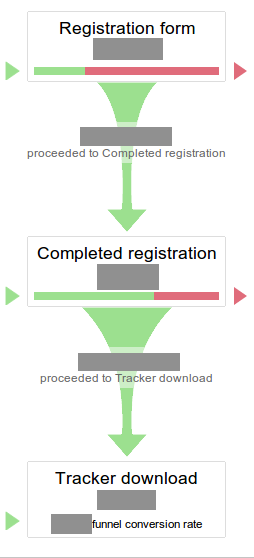
\includegraphics[width=50mm]{../images/goalfunnel}
    \end{wrapfigure}

    Bijvoorbeeld het doel van mensen aanmelden. Je kijkt dan vanaf welke pagina's mensen op het aanmeldformulier komen, en hoeveel van die mensen zich daadwerkelijk aanmelden. Het proces heet en Goal Funnel. Deze naam is gekozen omdat de gegevens vaan een trechtervorm hebben. Veel mensen komen op de homepagina, een kleiner aantal klikt door naar het formulier en een nog kleiner aantal schrijft zich daadwerkelijk in. Doel van het maken van zo'n goal funnel is om knelpunten te vinden. Zo kan er op \'e\'en bepaald punt in de rij van pagina's een probleem zitten waardoor de meeste mensen afhaken. Dit merk je omdat de trechter dan opeens v\'e\'e;l dunner wordt.

    Het doel van zo'n funnel analyseren is uitvinden op welke manier je de trechtervorm dikker kan krijgen, en dus meer mensen het door jouw gestelde doel kan laten bereiken. Doordat je op een goede manier kan laten zien waar de knelpunten zitten, kun je dit stap voor stap oplossen.

    \subsection{Bounce Rates}
    Bounce Rates is de term voor het percentage wat op een pagina komt, en niet verder klikt naar andere pagina's. Een hoge bounce rate betekent doorgaans dat de pagina niet is wat de gebruiker er van verwachte op het moment dat hij de pagina bezocht. Wanneer je weet welke pagina's een hoge bounce rate hebben, kan je onderzoeken \emph{waarom} die pagina's een hoge bounce rate hebben. Bijvoorbeeld omdat de naam van de pagina niet overeenkomt met de inhoud, of omdat de informatie op de pagina niet volledig genoeg is. Vaak is het zo dat een pagina simpelweg geen goede vervolgstap biedt, en het voor de gebruiker niet duidelijk is wat hij of zij nu moet doen.

    De belangrijkste pagina met betrekking tot Bounce Rates is doorgaans de homepagina. Dit is de pagina die nieuwe bezoekers voor het eerst zien, en de pagina die ze moet overhalen om zich aan te melden. Wanneer hier geen duidelijke vervolgstap op staat, of de gebruiker wordt niet genoeg gemotiveerd, zorgt dit voor een hogere bounce rate.

    Bij Wakoopa is de homepagina de pagina met de hoogste bounce rate, ongeveer een op de twee bezoekers klikken niet verder. Als je vervolgens kijkt waar bezoekers dan w\'el op klikken, dan is met 8\% de link naar de homepagina de hoogste. Hieruit kunnen we opmaken dat voor een percentage niet duidelijk is dat het hier om de homepagina gaat. Dit kunnen we oplossen door op de homepagina niet de link naar de homepagina te laten zien.

    Daarintegen klikt een op de vier bezoekers door naar de signup pagina, waar vervolgens meer dan de helft zich ook daadwerkelijk inschrijft (dit komt uit de signup funnel). Dat zijn hoge cijfers. Niettemin moet het lukken dit hoger te krijgen door ervoor te zorgen dat mensen op de homepagina minder snel wegklikken. Onder andere het onderzoek van \cite{Hoekman2008} doet een voorstel van hoe dit verbeterd kan worden.

    \subsection{Custom Tracking}
    Veel learning networks maken gebruik van \emph{AJAX}, een term die gebruikt wordt om aan te duiden dat delen van de pagina informatie van de server halen, maar niet de gehele pagina verversen. Het nadeel van deze techniek is dat er geen nieuwe \emph{page view} is, en dat dit dus ook niet automatisch met een statistiekprogramma wordt bijgehouden. In Google analytics heb je de mogelijkheid om via JavaScript zelf aan tracking te doen. Door een klein stukje code kan je aangeven dat iemand iets via AJAX heeft opgevraagd:
    \begin{verbatim}
    if(typeof(pageTracker) !== `undefined') {
      pageTracker._trackPageview(`/event/nameofevent');
    }
    \end{verbatim}
    Op deze manier kan je als learning network een hoop verschillende gebeurtenissen bijhouden. Bijvoorbeeld hoe vaak er op een banner wordt geklikt, of een comment wordt ingevoerd. Je krijgt hiermee inzicht in hoevaak een bepaalde functie wordt gebruikt.

    Op Wakoopa werd nog geen van de javascript opties getracked. Met behulp van van bovenstaande code is dit ingebouwd zodat we kunnen analyseren welke functies veel gebruikt worden. Ter verduidelijking zullen we een niet-bestaande boomstructuur gebruiken, in de vorm van \emph{/javascript/pagina-naam/naam-van-functie}. Door middel van de filters in Google Analytics kunnen deze dan gemakkelijk gevonden worden. In bijlage \ref{customtrackingappendix} staat een lijst van de functies die nu getracked worden.

    \subsection{Heatmaps}
      \begin{figure}
      \begin{center}
      \caption{Heatmap van de homepagina}
        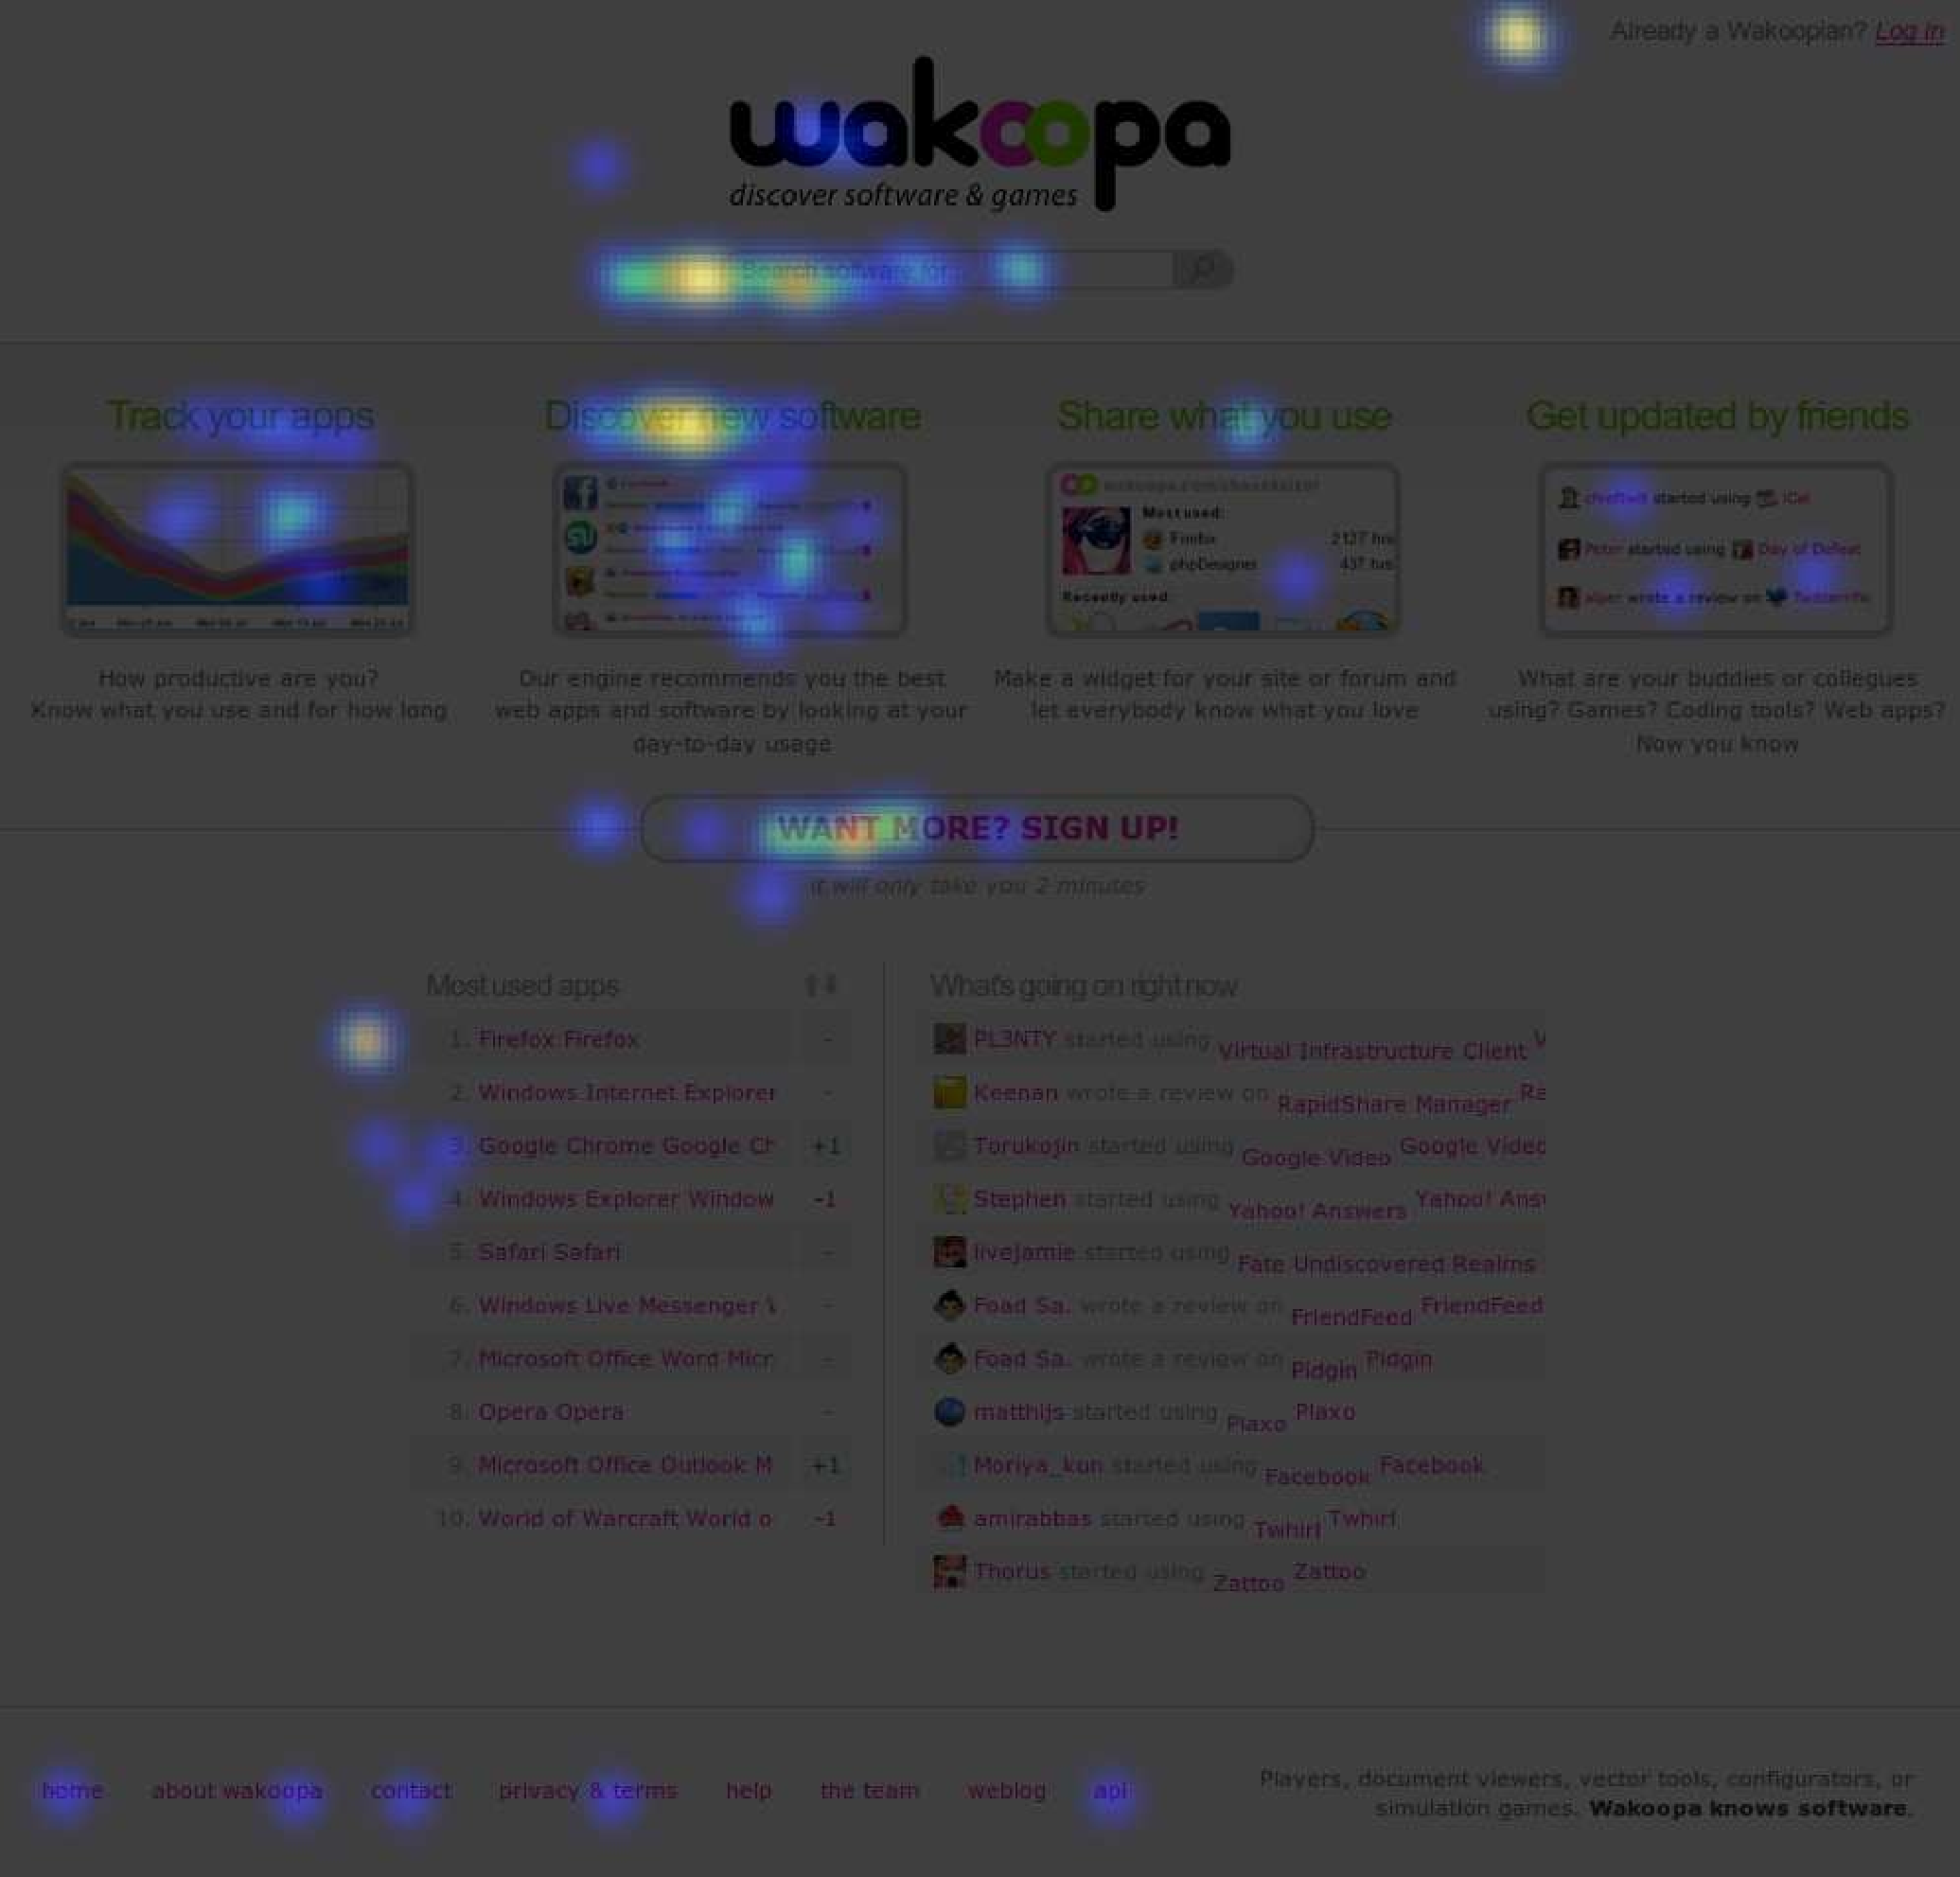
\includegraphics[width=70mm]{../images/heatmap}
      \label{heatmap}
      \end{center}
    \end{figure}
    Een techniek die pas sinds een paar jaar toegepast wordt is het maken van heatmaps. Deze heatmaps zien eruit als hittemappen, maar geven in plaats van temperatuur de hoeveelheid clicks of de positie van de muis aan op een website. Gedurende een vastgestelde periode houd je iedere click bij via javascript. Dit kan je dan later `plotten' op een screenshot, en zo zien waar het meest geklikt wordt. Omdat dit vrij intensief is voor de browser van de bezoeker, wordt het pas sinds recent toegepast, en nooit voor een lange duur.

    Door middel van deze techniek kan je goed zien welke delen van de pagina wel en welke delen niet worden gebruikt door je bezoekers. In Figuur \ref{heatmap} zie je een voorbeeld van de homepagina van Wakoopa, gemaakt met Crazyegg.\footnote{\url{http://crazyegg.com}} Wat hier opvalt is dat van de 4 afbeeldingen in het midden van de pagina, enkel de linker twee het meest worden aangeklikt. Hieruit kan je opmaken dat deze twee voor veel mensen interessanter zijn dan de rechter twee. Omgekeerd, de rechter twee zijn niet duidelijk genoeg, of wekken vergeleken met de linker twee niet even veel interesse. Een verbeterpunt. Het is dan aan de ontwikkelaar om te beslissen of dit betekent dat de rechter twee verbeterd moeten worden, weggehaald, of minder nadruk moeten krijgen waarbij de linker twee meer nadruk krijgen.

    Het is belangrijk om voordat je een heatmap laat genereren, te bepalen wat de doelen op een pagina zijn, waar de bezoeker moet klikken en welke delen welke soort bezoeker moeten aanspreken. Wanneer je dit doet is het achteraf gemakkelijk om te kijken in hoeverre bezoekers de pagina gebruiken op de manier dat jij bedoelde, en of de doelen die je hebt opgestelt ook daadwerkelijk behaald worden.


    \section{A/B testing}
    \textit{A/B testing, of multivariate testing, is een methode om twee (A/B) of meerdere (multivariate) variaties op een pagina of lay-out te testen, door deze gedurende een periode willekeurig onder bezoekers te verdelen. Bezoeker \emph{A} krijgt bijvoorbeeld variatie 1 te zien, en bezoeker \emph{B} krijgt variatie 2 te zien. Vervolgens kijk je welke gebruiker sneller of vaker op de door jouw gekozen link klikt of actie uitvoerd. Wanneer je dit met een groot aantal bezoekers gedurende een langere tijd doet, kan je hier statistische analyse op uitvoeren.}

   Het ontwikkelplatform wat Wakoopa gebruikt, Ruby on Rails, heeft door middel van een plugin de optie om A/B testen uit te voeren. Deze automatiseert het verdelen van de verschillende opties tussen bezoekers en houd per variatie bij hoe vaak de geteste links of functionaliteit aangeklikt wordt.

    Naar aanleiding van de in Hoofdstuk \ref{researchchapter} genoemde onderzoeken hebben we een aantal A/B tests uitgevoerd, die hieronder beschreven staan:

    \subsection{Plaats van de sign-up link op landing pages}
      \label{ctatest}
      In tegenstelling tot de homepagina hebben onze landing pages (Pagina's waar bezoekers via zoekmachines op terecht komen) wel een sign-up link in de header. Momenteel staat deze in de linkerbovenhoek. In deze A/B test bekijken we of een variate waarin deze in de rechterbovenhoek staat, tot meer clicks leidt dan wanneer deze in de linkerbovenhoek staat. De resultaten staan in Tabel \ref{tab:signupcta}, de conclusie in Hoofdstuk \ref{wak:Editorial2008}.

        \begin{table}[ht]
        \centering
        \caption{Resultaten van de sign-up link}
        \begin{tabular}{r|*{3}{c}}
          \textbf{Versie}  & Conversie  & Verbetering & Clicks / Pageviews \\ \hline
          \textbf{Links}   & 0.00036\%  & \emph{n.v.t.}        & 1544 / 4200125 \\
          Rechts  & 0.00025\%  & -32\%                & 1058 / 4199310 \\
        \end{tabular}

        \label{tab:signupcta}
        \end{table}
    \begin{figure}
      \caption{Links}
      
\includegraphics[width=\textwidth]{../images/abtest/left}
      \caption{Rechts}
      
\includegraphics[width=\textwidth]{../images/abtest/right}
    \end{figure}

    \subsection{Het benoemen van de mate waarin een profiel is ingevuld}
      \label{profileprogress}
      Wakoopa geeft gebruikers al een berichtje na het inloggen wanneer een profiel nog niet volledig is ingevuld. Uit onderzoek van \cite{Brouns2008} blijkt dat het effectiever is om hier een vervolgstap of een progressiemeter neer te zetten. In deze test bekijken we een viertal variaties: De huidige berichtgeving, een berichtgeving met welk eerstvolgende veld ze nog moeten invullen (bv. Bio), een berichtgeving met een progressiemeter, en een berichtgeving met zowel een progressiemeter als wel eerstvolgende veld ingevuld moet worden.  De resultaten staan in Tabel \ref{tab:profilecta}, de conclusie in Hoofdstuk \ref{wak:Brouns2008}

        \begin{table}[ht]
        \centering
        \caption{Resultaten van het benoemen van de mate waarin een profiel is ingevuld}
        \rowcolors{1}{white}{lightgray}
        \begin{tabular}{r|*{3}{c}}
          \textbf{Versie}                   & Conversie  & Verbetering   & Clicks / Pageviews \\ \hline
          Origineel                         & 9\%        & \emph{n.v.t.} & 502 / 5357 \\
          Met suggestie                     & 7\%        & -22\%         & 430 / 5402\\
          \textbf{Met progressiemeter}      & 15\%       & 66\%          & 819 / 5355\\
          Met beide  & 12\%       & 33\%          & 635 / 5284\\
        \end{tabular}
        \label{tab:profilecta}
        \end{table}

    \begin{figure}
      \caption{origineel}
      
\includegraphics[width=\textwidth]{../images/abtest/original}

      \caption{met suggestie}
      
\includegraphics[width=\textwidth]{../images/abtest/suggestion}

      \caption{met progressiemeter}
      
\includegraphics[width=\textwidth]{../images/abtest/progresbar}

      \caption{met suggestie en progressiemeter}
      
\includegraphics[width=\textwidth]{../images/abtest/both}
    \end{figure}

  \newpage
  \chapter{Usabilitytechnieken die de participatie op een learning network verhogen}


  \newpage
  \chapter{Welke verbeteringen zijn er specifiek voor Wakoopa door te voeren?}
    \newpage

    Dit hoofdstuk gaat expliciet in op verbeteringen voor Wakoopa, zoals gebleken uit de vorige hoofdstukken. We passen de theorie uit hoofdstuk \ref{researchchapter}, de gebruikersonderzoeken van hoofdstuk \ref{userchapter} en de data van hoofdstuk \ref{datachapter} toe op Wakoopa en beschrijven de bevindingen en aanbevelingen.

    \section{Onderzoeken}
    Naar aanleiding van de onderzoeken in hoofdstuk \ref{researchchapter} zijn er voor Wakoopa de volgende verbeteringen:

 \subsection{\cite{Beenen2004}}
      In dit onderzoek wordt veel nadruk gelegd op de \emph{call to actions}. Deze moeten een interne motivatie stimuleren, maar er niet voor zorgen dat het lijkt alsof dit een externe motivatie is. De call to actions op de homepagina zijn een goed voorbeeld om te onderzoeken of deze inderdaad voldoen aan dit vereiste.

      \paragraph{\textbf{Verbeterpunten:}}
      \begin{itemize}
        \item Call to actions op homepagina aanpassen
      \end{itemize}

    \subsection{\cite{Berlanga2007}}
    Een aantal van de punten uit het onderzoek van \citeauthor{Berlanga2007} werden in het geval van Wakoopa al gebruikt. Het is gemakkelijk om nieuwe connecties te leggen (dit kan via een enkele klik op iemands profiel) en dit wordt gestimuleerd door aan te geven welke gebruikers op jou lijken. Gebruikers krijgen een bericht wanneer hun vrienden nieuwe applicaties gebruiken, een review schrijven, een level omhoog gaan of iets op een teampagina schrijven. De effectiviteit van dit punt wordt ook ondersteund door onderzoek van \cite{Berlanga2007}. Nieuwsgierigheid wordt gestimuleerd door het puntensysteem, waarbij gebruikers meer punten verdienen door meer software te gebruiken en door acties op de site uit te voeren. Er wordt hier enkel het level getoond, en niet het totaal aantal punten. Door dit toe voegen bied je ook voor mensen die op eht hoogste level zitten een manier om zich met anderen te vergelijken. Een ander punt waar verbetering te behalen valt is het langer vasthouden van bezoekers. Wakoopa kan dit verbeteren door mensen meer acties op de site uit te laten voeren, en interessante(re) statistieken weer te geven op profielen.

      \paragraph{\textbf{Verbeterpunten:}}
      \begin{itemize}
        \item Totaal aantal punten op het profiel laten zien
        \item Bestaande functionaliteit uitbreiden
        \item Meer statistieken bieden
      \end{itemize}


    \subsection{\cite{Brouns2008}}
    \label{wak:Brouns2008}
    Wakoopa toonde enkel een melding dat een profiel nog niet compleet was, zonder vervolgstappen aan te geven. Door het implementeren van een progressiemeter zijn er 15\% meer mensen die doorklikken naar hun accountgegevens.

    Dit resultaat bleek uit een A/B test in hoofdstuk \ref{datachapter} (zie pagina \pageref{profileprogress}). Uit deze A/B test bleek dat enkel het tonen van een progressiemeter effectiever is dan het tonen van enkel een bericht, een bericht met een suggestie van een leeg veld of het tonen van een bericht met zowel een progressiemeter en een suggestie. Mogelijke verklaringen hiervoor zijn dat de zin te lang wordt wanneer er ook een suggestie in staat, of dat de suggestie velden aangeeft die mensen niet in willen vullen.

      \paragraph{\textbf{Verbeterpunten:}}
      \begin{itemize}
        \item Toevoegen van een progressiemeter met in hoeverre het profiel is gevuld
      \end{itemize}

    \subsection{\cite{Editorial2008}}
    \label{wak:Editorial2008}
    Het merendeel van de onderzochte sociale netwerken heeft een signup call to action in de rechterbovenhoek staan. Bij Wakoopa staat deze onder het logo aan de linkerkant. Door middel van een A/B test (zie pagina \pageref{ctatest}) is gekeken of dit ook voor Wakoopa meer clicks opleverde. Opvallend genoeg bleek rechts ongeveer twee keer zo slecht te werken als links. Hier zijn twee mogelijke verklaringen voor. De eerste is dat de call to action links al direct onder het logo stond, een plek waar veel mensen bij het openen van een nieuwe site als eerste kijken\footnote{\url{http://www.useit.com/alertbox/reading\_pattern.html}}. Een andere verklaring is \emph{banner blindness}. Omdat de call to action rechts naast de banner stond en het leek alsof de call to action daarbij hoorde, zullen mensen eerst de banner zien en dan automatisch de banner negeren, en daarmee ook de call to action negeren.\footnote{\url{http://www.useit.com/alertbox/fancy-formatting.html}}

      \paragraph{\textbf{Verbeterpunten:}}
      \begin{itemize}
        \item Geen
      \end{itemize}

    \subsection{\cite{Wroblewski2009}}
    Wakoopa past bij het aanmelden van een nieuwe account al de meest effectieve vorm van inline validatie toe, maar op andere plekken wordt dit nog niet gedaan. Op de account pagina kan inline validatie goed worden toegepast, om aan te geven of een nieuw wachtwoord goed genoeg is, of een wachtwoord en het controlewachtwoord overeenkomen en om aan te geven en of het ingevoerde emailadres voldoet.

      \paragraph{\textbf{Verbeterpunten:}}
      \begin{itemize}
        \item Validatie toevoegen aan de account settings pagina
      \end{itemize}

    \subsection{\cite{Alfrink2008}}
    Sinds dit rapport heeft Wakoopa een speciale pagina aangemaakt die de gebruiker direct ziet na het aanmelden, waar in punten uit wordt gelegd welke vervolgstappen een nieuwe gebruiker heeft (de tracker downloaden, contacten zoeken, naar zijn dashboard gaan). Op andere punten kan Wakoopa dit beter stimuleren, bijvoorbeeld door middel van e-mails wanneer een gebruiker een week of twee weken lang de service niet heeft gebruikt, of alerts wanneer een gebruiker een applicatie veel gebruikt maar nog niet heeft gereviewt. Deze twee directe vragen om participatie zouden volgens \citeauthor{Alfrink2008} zeer geschikt zijn om in te zetten.

    Naast deze oproepen tot participatie noemt \citeauthor{Alfrink2008} het weergeven van persoonlijke informatie op algemene pagina's als een punt van verbetering. Sinds dit rapport wordt er al veel persoonlijke informatie weergegeven op bijvoorbeeld de software en developer-pagina's, maar niet op bijvoorbeeld de categoriepagina's, waar je heel goed een top-5 van door jouw gebruikte applicaties in die categorie kan laten zien.
    \paragraph{\textbf{Verbeterpunten:}}
      \begin{itemize}
        \item Alerts geven wanneer een gebruiker een applicatie langer dan vijf uur gebruikt heeft maar nog geen review heeft geschreven
        \item E-mail sturen wanneer een gebruiker twee weken geen software heeft getrackt.
        \item Een persoonlijke top 5 toevoegen op de categoriepagina's
      \end{itemize}

    \subsection{\cite{Hoekman2008}}
    Het grootste kritiekpunt uit dit onderzoek was de navigatie en de indeling van de homepagina. De homepagina had niet \'e\'en duidelijk focuspunt en de vier punten geven niet duidelijk genoeg de voordelen van Wakoopa weer. Voor de navigatie stellen ze voor om deze te herstructureren naar drie niveau's, gefocust op gebruikersdoelen.

    \paragraph{\textbf{Verbeterpunten:}}
      \begin{itemize}
        \item Navigatiestructuur focussen op gebruikersdoelen
        \item Homepagina re-align maken, waarin de aandacht gaat naar voordelen in een duidelijk blok, en er meer uitleg is.
      \end{itemize}


    \subsubsection{Verbetering van de navigatie}
      \citeauthor{Hoekman2008} doen een voorstel tot verbetering van de navigatie. in figuur \ref{currentnav} is de huidige navigatiestructuur van Wakoopa uitgetekend, en in figuur \ref{miskeetonav} de navigatiestructuur zoals voorgesteld in  \cite{Hoekman2008}. De sitemaps zijn gemaakt met Slickmap.\footnote{\url{http://astuteo.com/slickmap/}} Belangrijk is hierbij op te merken dat de voorgestelde navigatie niet volledig is, en als uitgangspunt bedoeld is. Zo missen de tags, updates en recommendations, die in de huidige site ook nog geen correcte plek hebben. Een ander punt wat opvalt is het gebruik van `My' om persoonlijke onderdelen aan te duiden. Wakoopa gebruikt hier `Your' voor, om het verschil tussen het learning network (wij) en de gebruiker (zij) aan te geven. Er is geen eenduidig antwoord voor welke variant beter is, en verschillende social networks gebruiken verschillende aanduidingen. Myspace en Facebook gebruiken `my', Hyves zowel `mijn' als `je', en last.fm gebruikt `your'.

      \begin{figure}
      \begin{center}
      \caption{Huidige navigatie}
        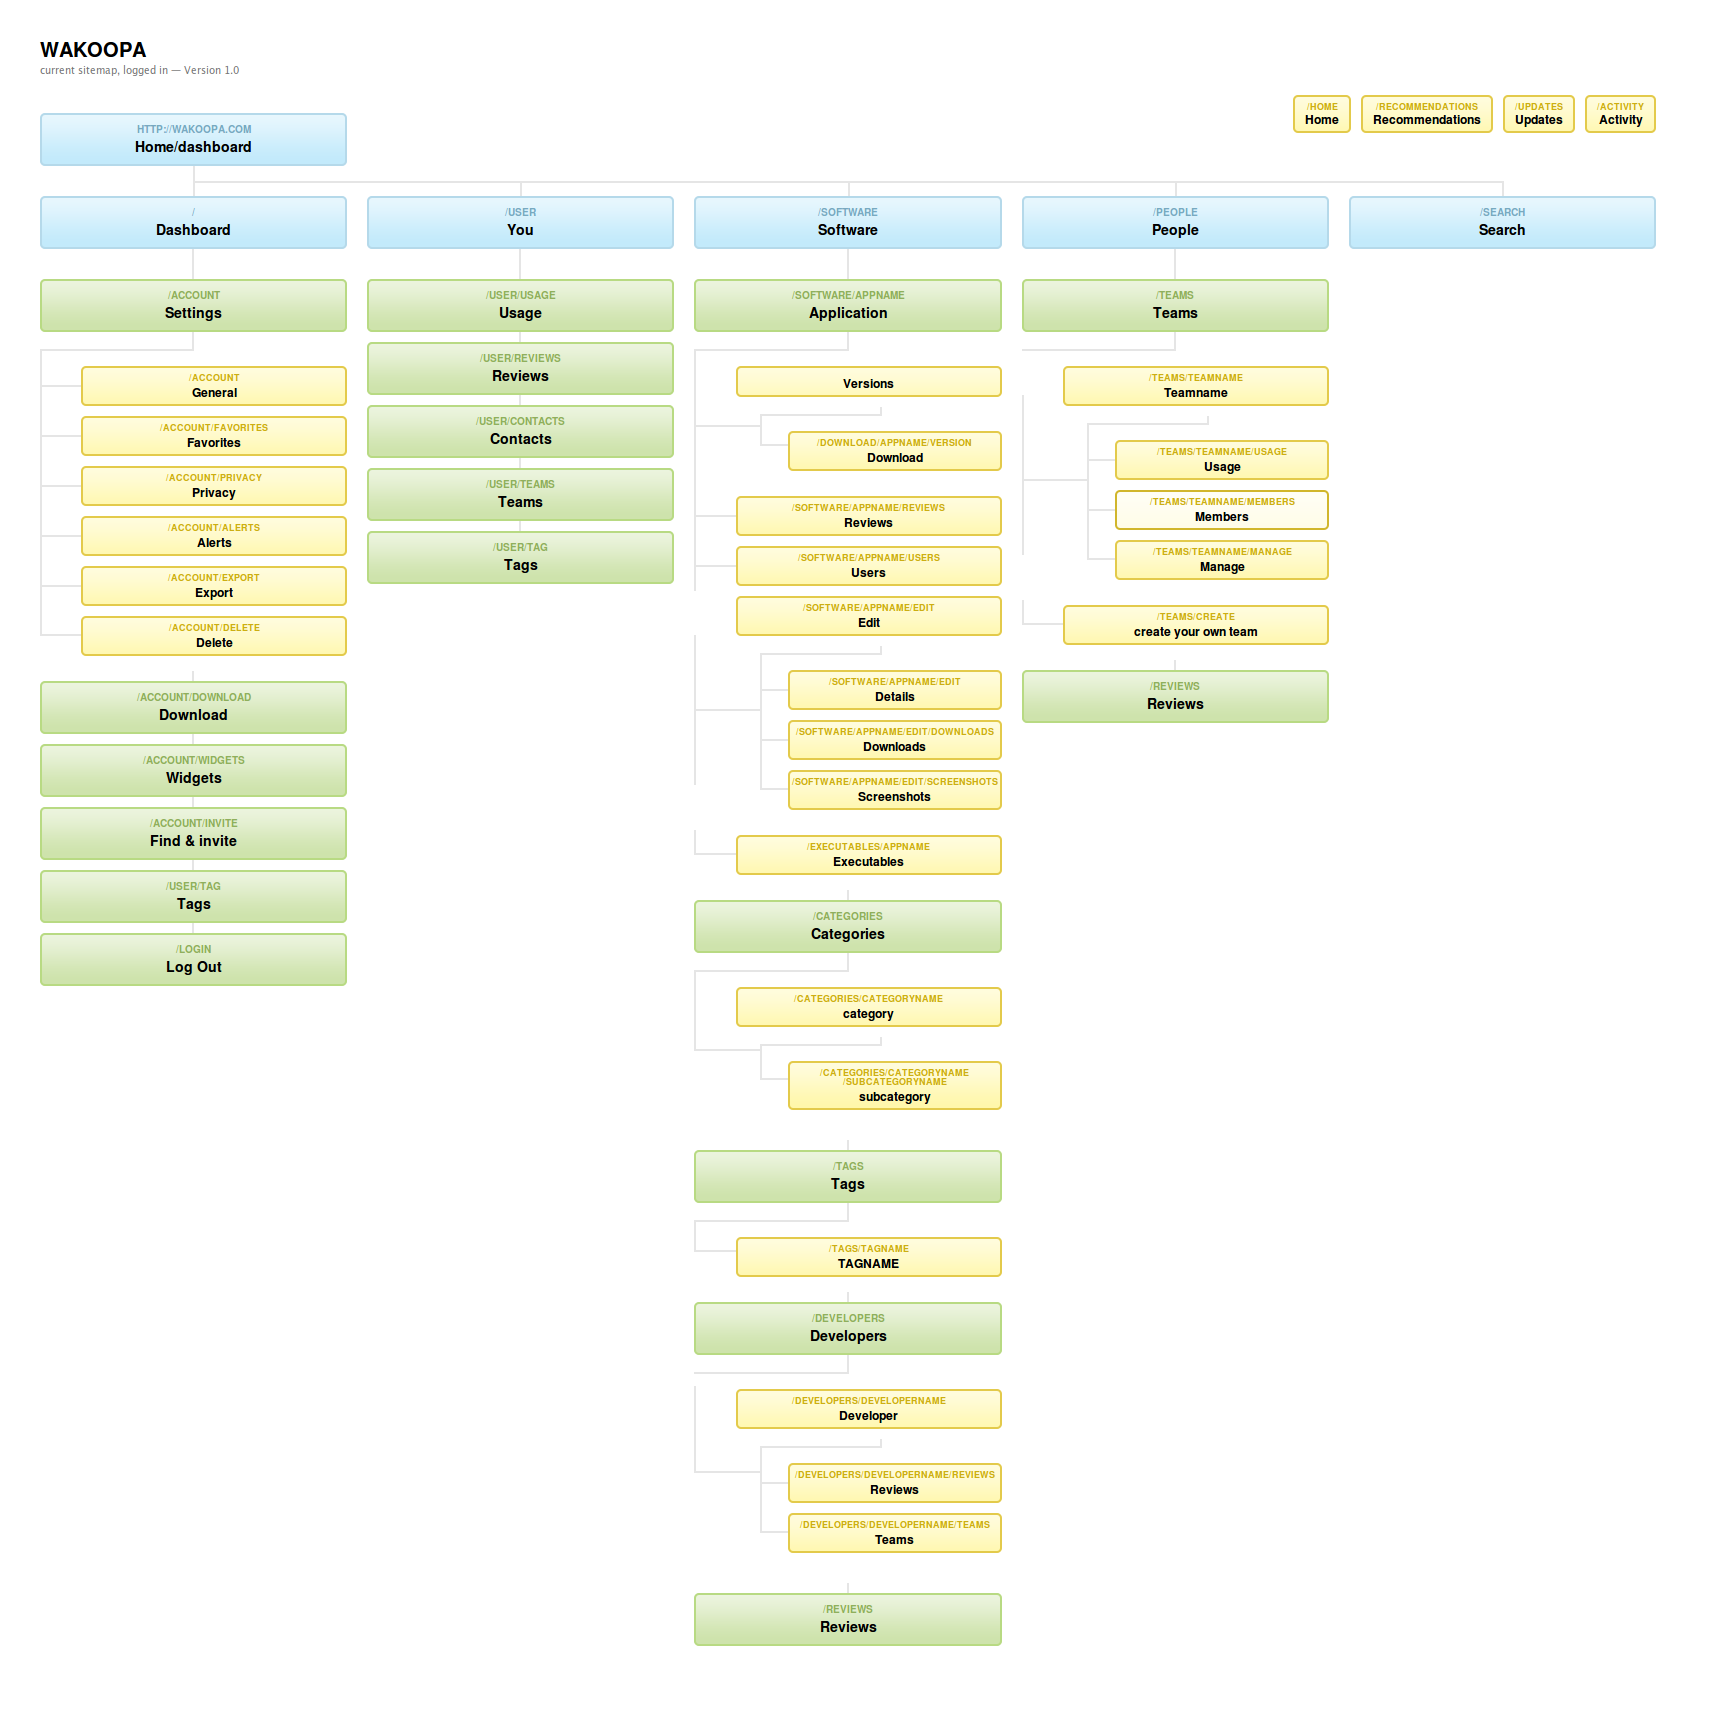
\includegraphics[width=\textwidth]{../images/currentnav}
      \label{currentnav}
      \end{center}
    \end{figure}

    \begin{figure}
      \begin{center}
      \caption{Verbeterde navigatie volgens \cite{Hoekman2008}}
        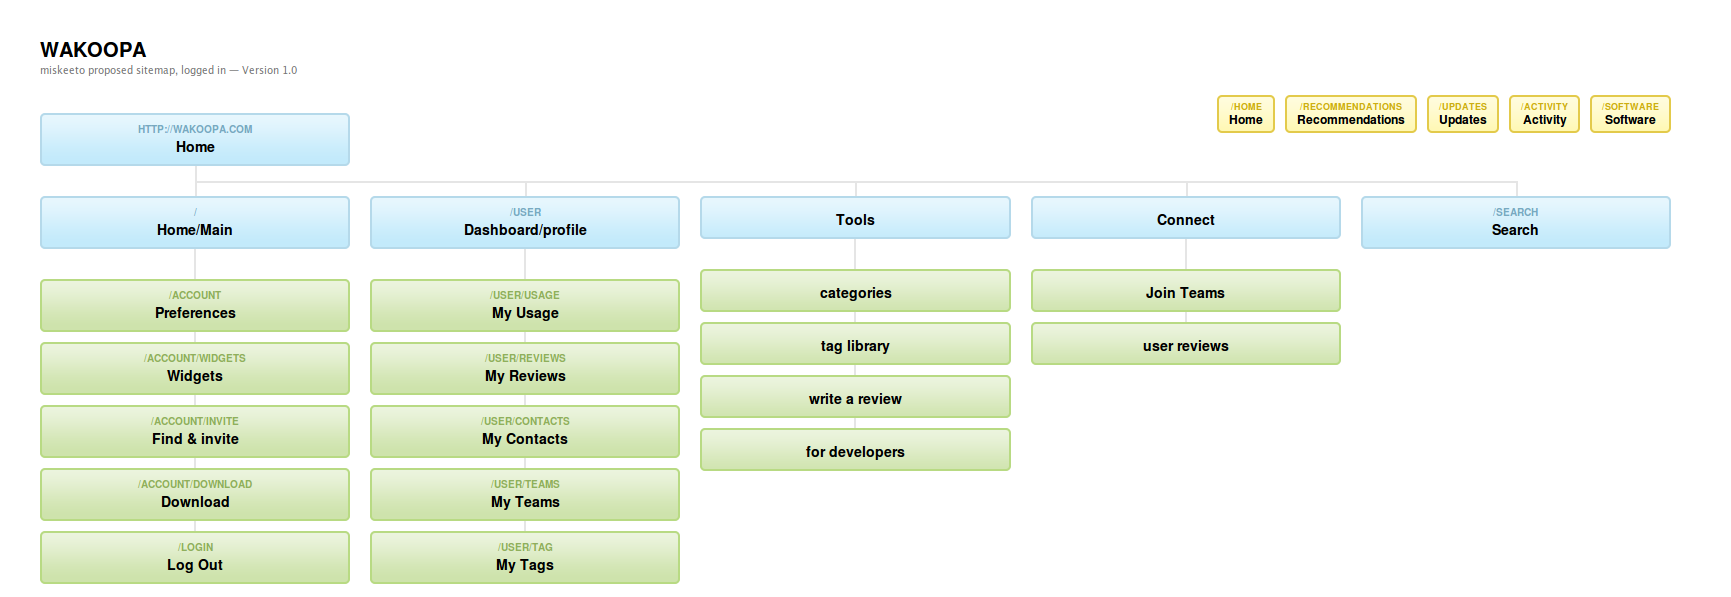
\includegraphics[width=\textwidth]{../images/miskeetonav}
      \label{miskeetonav}
      \end{center}
    \end{figure}

    \subsubsection{Navigatie workshop}
      Om te onderzoeken op welke manier de navigatie verbeterd kan worden is een navigatieworkshop met alle Wakoopa-medewerkers gehouden. Dit onderzoek is beschreven in bijlage \ref{navigationappendix}. Uit dit onderzoek kwamen een aantal kleine verbeteringen naar voren. Teams, categories en developers worden meer naar voren gepracht dan in de huidige navigatie. Het downloaden van de tracker is voor iedereen toegankelijk geworden, en als laatste wordt er een duidelijkere verdeling gemaakt tussen wat er bij een gebruiker zijn publieke profiel, en bij het persoonlijke gedeelte van een account hoort.

    \subsection{\cite{Timmerman2008}}
    In dit onderzoek wordt veel verwezen naar het analyseren van data en gebruik van andere usabilitytechnieken dan een expert review. Het analyseren van Statistieken, het gebruik van A/B testen en het maken van persona's worden als nuttige middelen genoemt. Door middel van deze persona's kan bij (nieuwe) functionaliteit worden gekeken of dit wel overeenkomt met gebruikersdoelen.

    \paragraph{\textbf{Verbeterpunten:}}
      \begin{itemize}
        \item Maak persona's en gebruikersdoelen
        \item Analyseer de statistieken op trends
      \end{itemize}

    \subsubsection{Persona's}
      In bijlage \ref{personasappendix} zijn persona's voor Wakoopa gemaakt. Deze zijn opgestelt aan de hand van \cite{Klompsma} en gebaseerd op de enqu\^ete en de doelgroepsanalyse die door Wakoopa intern is gemaakt. \cite{Klompsma} combineert het maken van persona's gebaseerd op doelgroepen met een analyse van het soort persoon. Dit doet hij aan de hand van een variatie op de Myer Briggs type indicator (Dit is een psychologische test die je in een van de zestien voorkeurscategorie\"en indeelt) zoals beschreven in \cite{Williams}. In dit boek vertaalt auteur Roy Williams de zestien categorieren naar vier soorten gebruikers, op basis van twee vragen:
      \begin{itemize}
        \item Ben je een snelle of langzame beslisser?
        \item Beslis je op basis van feiten of op basis van emotie?
      \end{itemize}

      \paragraph{}De vier gebruikers die hier uit voortkomen zijn:

      \begin{itemize}
        \item de competitieve gebruiker
          Deze mensen beslissen snel en op basis van feiten
        \item De methodische gebruiker
          Deze mensen beslissen langzaam en op basis van feiten
        \item De spontane gebruiker
          Deze mensen beslissen snel en op basis van emotie
        \item De humanistische gebruiker
          Deze mensen beslissen langzaam en op basis van emotie
      \end{itemize}

      In de persona's voor Wakoopa komen twee competitieve, een spontane en een humanistische gebruiker voor. Het is voor deze doelgroepen belangrijk dat de juiste informatie snel op een goede manier wordt gepresenteerd.

    \section{Statistieken}
    \subsection{Custom tracking}
    Na het toevoegen van custom tracking was er meer inzicht in welke javascriptfunctionaliteit het meest gebruikt werd. Voornamelijk interessant was welke grafieken het meest bekeken werden. grafieken van dagelijks gebruik zijn meer dan twee keer zo populair als de overige grafieken. Een verbetering hier zou dus zijn standaard deze grafiek te laten zien. Wat ook opvalt is dat het bekijken van redenaties achter aanbevelingen, en het verwijderen van niet geschikte aanbevelingen erg vaak gebeurd. Het verwijderen van aanbevelingen gebeurd bijna evenveel als het bekijken van redenaties achter aanbevelingen.

    Het toevoegen van favorites gebeurd bijna driemaal zovaak als het toevoegen van tags. Dit is te verklaren met het feit dat favorites op de site vrij gemakkelijk te vinden zijn, terwijl dit bij tags nog niet het geval is. Een conclusie zou kunnen zijn dat mensen favorites als een `gemakkelijke' of socialere vorm van taggen zien.

    \paragraph{\textbf{Verbeterpunten:}}
      \begin{itemize}
        \item Toon de meest interessante grafiek als eerste
        \item Maak tagging duidelijker
      \end{itemize}


  \newpage
  \chapter{De quick wins om participatie te verhogen op learning networks}
    \newpage

  \newpage
  \chapter*{Conclusie en Aanbevelingen}
  \addcontentsline{toc}{chapter}{Conclusie en Aanbevelingen}

  \newpage
  \chapter*{Discussie}
  \addcontentsline{toc}{chapter}{Discussie}

  \newpage
  \chapter*{Verklarende woordenlijst}
  \addcontentsline{toc}{chapter}{Verklarende woordenlijst}

  \listoftables
  \addcontentsline{toc}{chapter}{Lijst van tabellen}

  \listoffigures
  \addcontentsline{toc}{chapter}{Lijst van figuren}


  \newpage
  \bibliography{../references/referenties}
  \bibliographystyle{../references/agsm2}
  \addcontentsline{toc}{chapter}{Bibliografie}
  \newpage

  \appendix
  \addappheadtotoc
  \chapter{Analyse homepagina: call to actions}
\label{analysehomeappendix}
\textit{3 november 2009} De vier punten op de huidige homepagina van Wakoopa noemen enkel functionaliteit, in plaats van voordelen (\citet{Hoekman2008}) of uniekheid van gebruikers (\citet{Beenen2004}). Door de call-to-actions aan te passen naar een van deze twee uitgangspunten, zou het aantal aanmeldingen (en dus de participatie) moeten verhogen.

\paragraph{huidig:}
\begin{itemize}
    \item{Track your apps\\
      How productive are you?\\
      Know what you use and for how long}

    \item{Discover new software\\
      Our engine recommends you the best web apps and software by looking at your day-to-day usage}

    \item{Share what you use\\
      Make a widget for your site or forum and let everybody know what you love}

    \item{Get updated by friends\\
      What are your buddies or colleagues using? Games? Coding tools? Web apps? Now you know}
\end{itemize}

Naast de bewoording van deze punten, kunnen we ook inhoudelijk kijken naar de punten. Wanneer we de survey bekijken, blijkt dat slechts een derde van de huidige gebruikers wel eens een widget op zijn blog of facebook heeft gezet. Voor het overgrote deel van de gebruikers was dit dus niet een reden om zich aan te melden, en daarmee zijn er wellicht andere functies die bezoekers meer prikkelen. Nieuwe functionaliteit waar huidige gebruikers het meest enthousiast over zijn zijn de aanbevelingen en het web tracking. Deze twee functionaliteiten komen niet duidelijk naar voren. De aanbevelingen worden genoemd, maar slechts indirect, en hetzelfde geld voor web apps.Kijkend naar de enqu\^ete kunnen deze beter prominent in beeld worden gebracht.

Na Web tracking en aanbevelingen zijn de twee grootste nieuwe functionaliteiten waar gebruikers tevreden over zijn het tracken op linux en het reputatie en puntensysteem. Kijkend naar de huidige homepagina staat er nergens op welke platformen wakoopa ge\"installeerd kan worden, en welke worden getrackt. ook het reputatie en puntensysteem wordt niet genoemd, terwijl een significant deel van de gebruikers aangeeft dit een waardevolle toevoeging te vinden.

Met bovenstaande punten kunnen we een nieuw lijstje maken met daarin de functionaliteiten die het belangrijkst zijn en die door huidige gebruikers het meest gewaardeerd worden:
\begin{itemize}
    \item{Track what you use\\
      Keep track of what you use on Windows, Mac OS X, Linux and the web}

    \item{Get recommendations\\
      We analyse your day-to-day usage and recommend you new software}

    \item{Updates from friends\\
      See which applications your friends use and what they think of them}

    \item{Collect awards\\
      Level up to become a Wakoopa overlord and compare with friends}
\end{itemize}

Deze functionele items kunnen we vervolgens omvormen naar een lijst met persoonlijke voordelen, en een lijst met nadruk op de uniekheid van gebruikers:

\paragraph{Voordelen (\citet{Hoekman2008}) }
\begin{itemize}
    \item{Gain insight\\
      Keep track of what you use on Windows, Mac OS X, Linux and the web}

    \item{Find better applications\\
      We analyse your day-to-day usage and recommend you new software}

    \item{Match with friends\\
      See which applications your friends use, what they think of them}

    \item{Become an overlord\\
      Use Wakoopa, get awards and reach the highest level}
\end{itemize}
\paragraph{Uniekheid (\citet{Beenen2004})}
\begin{itemize}
    \item{Find your usage patterns\\
      Keep track of what you use on Windows, Mac OS X, Linux and the web}

    \item{Personal recommendations\\
      We analyse your day-to-day usage and recommend you new software}

    \item{Do you differ from friends?\\
      See which applications your friends use and what they think of them}

    \item{Compete with friends\\
      Use Wakoopa, get awards and become a Wakoopa overlord}
\end{itemize}

    \begin{figure}
      \begin{center}
      \caption{Grafische weergave}
        \subfigure[Origineel]{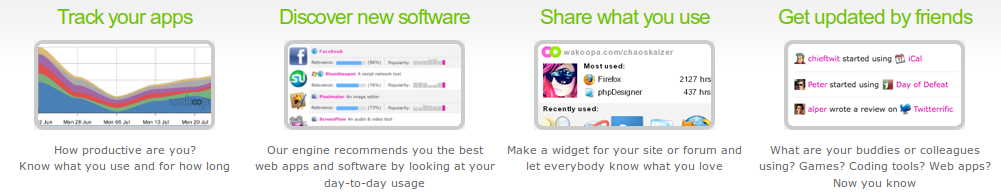
\includegraphics[width=\textwidth]{../images/newhomepage/original}}
        \subfigure[Andere items]{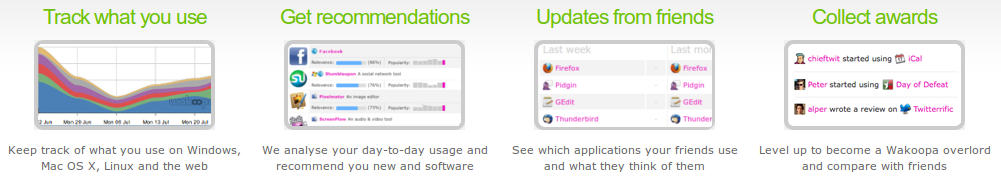
\includegraphics[width=\textwidth]{../images/newhomepage/improved}}
        \subfigure[Voordelen]{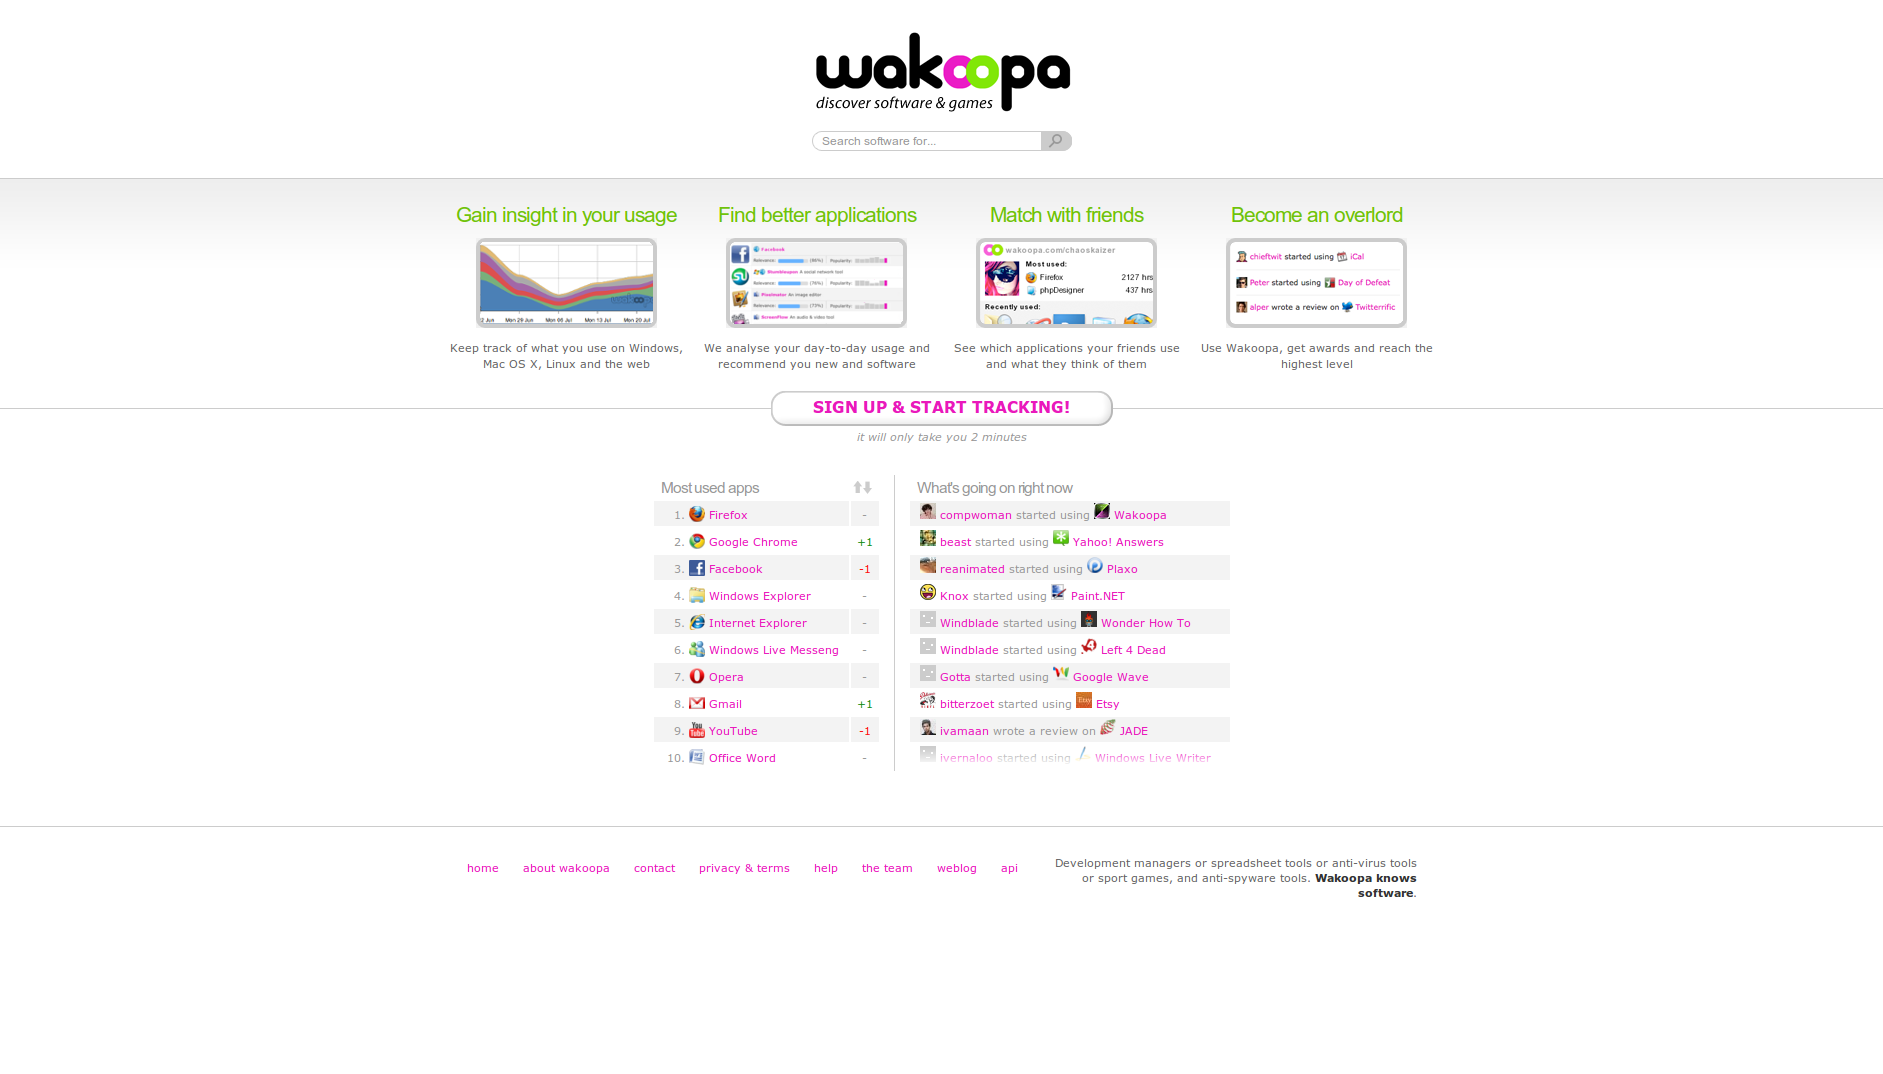
\includegraphics[width=\textwidth]{../images/newhomepage/benefits}}
        \subfigure[Uniekheid]{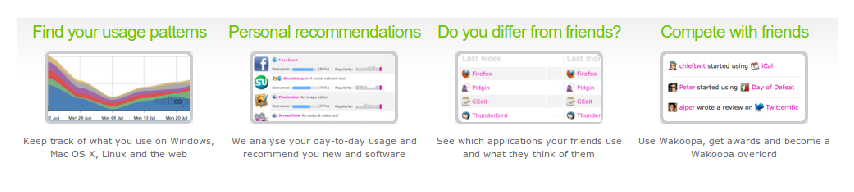
\includegraphics[width=\textwidth]{../images/newhomepage/uniqueness}}
      \end{center}
    \end{figure}


  \chapter{Navigatie brainstorm}
    \label{navigationappendix}
\textit{28 oktober 2009} Door middel van een brainstorm over de navigatie van Wakoopa is er een sitemap opgesteld. De brainstorm is uitgevoerd door het Team van Wakoopa (Wouter, Robert, Menno, Mark en Marten), wat betekent dat er voorkennis aanwezig was. Dit is deels tegengegaan doordat er twee personen bij waren die minder bekend waren met de huidige navigatie, Mark en Marten. Er is uitgegaan van een ingelogde status, een status waarbij de gebruiker toegang heeft tot zijn eigen gegevens. Statische pagina's zoals Privacy, About en FAQ zijn voor deze brainstorm buiten beschouwing gelaten, omdat ze niet actief deel hebben in gebruik van de website.

Van tevoren waren alle bestaande pagina's op post-its geschreven, en deze zijn verdeeld over de aanwezigen met de opdracht om deze gezamelijk op een A1 vel te plakken, waarbij gelijk pagina's geclusterd werden en de hi\"erarchie aangegeven werd door post-its onder elkaar te plakken. Hier werd expliciet gevraagd niet aan de huidige navigatie vast te houden, maar het zo neer te leggen dat het voor de personen zo logisch mogelijk was. Bijgevoegd waren pennen, waarmee de deelnemers toevoegingen of verduidelijkingen op of om de post-its konden schrijven.

\section*{Uitkomst}
De website werd ingedeeld in zeven hoofdsecties: Home, dashboard, application, people, teams, categories en developers.. Dit is iets anders dan de huidige site, die Home/dashboard, Software, People en Search als hoofdsecties heeft. Het downloaden van de tracker staat momenteel onder het dashboard, maar werd liever direct onder Home gezien, met de beredenatie dat iedereen in principe de tracker mag downloaden. Een ander tweedeling is die van informatie over een gebruiker. Een deel daarvan hoort onder het dashboard (jouw persoonlijke accountpagina) en het ander onder You, je publieke profiel. Uit de workshop bleek dat een aantal van deze dingen niet op de goede plek stonden en beter zouden kloppen wanneer ze onder het persoonlijke dan wel publieke deel van Wakoopa zouden staan.
\section*{Vergelijking met \citeauthor{Hoekman2008}}
Kijkend naar de verbeteringen zoals voorgesteld door \citeauthor{Hoekman2008} (zie figuur \ref{miskeetonav2}) kun je zien dat de uitkomst van de workshop tussen de huidige site en de verbeteringen van \citeauthor{Hoekman2008} in zit. Hoewel de benaming en de pagina's hetzelfde blijven als op de huidige site, met slechts hier en daar een bijgeschreven verbetering, neigt de verdeling van de pagina's meer naar de indeling van \citeauthor{Hoekman2008}. Waar de verbeterde versie van \citeauthor{Hoekman2008} een compleet nieuwe indeling is, kwam er uit de workshop een gefinetunede versie van de huidige navigatie.

      \begin{figure}
      \begin{center}
      \caption{Huidige navigatie}
        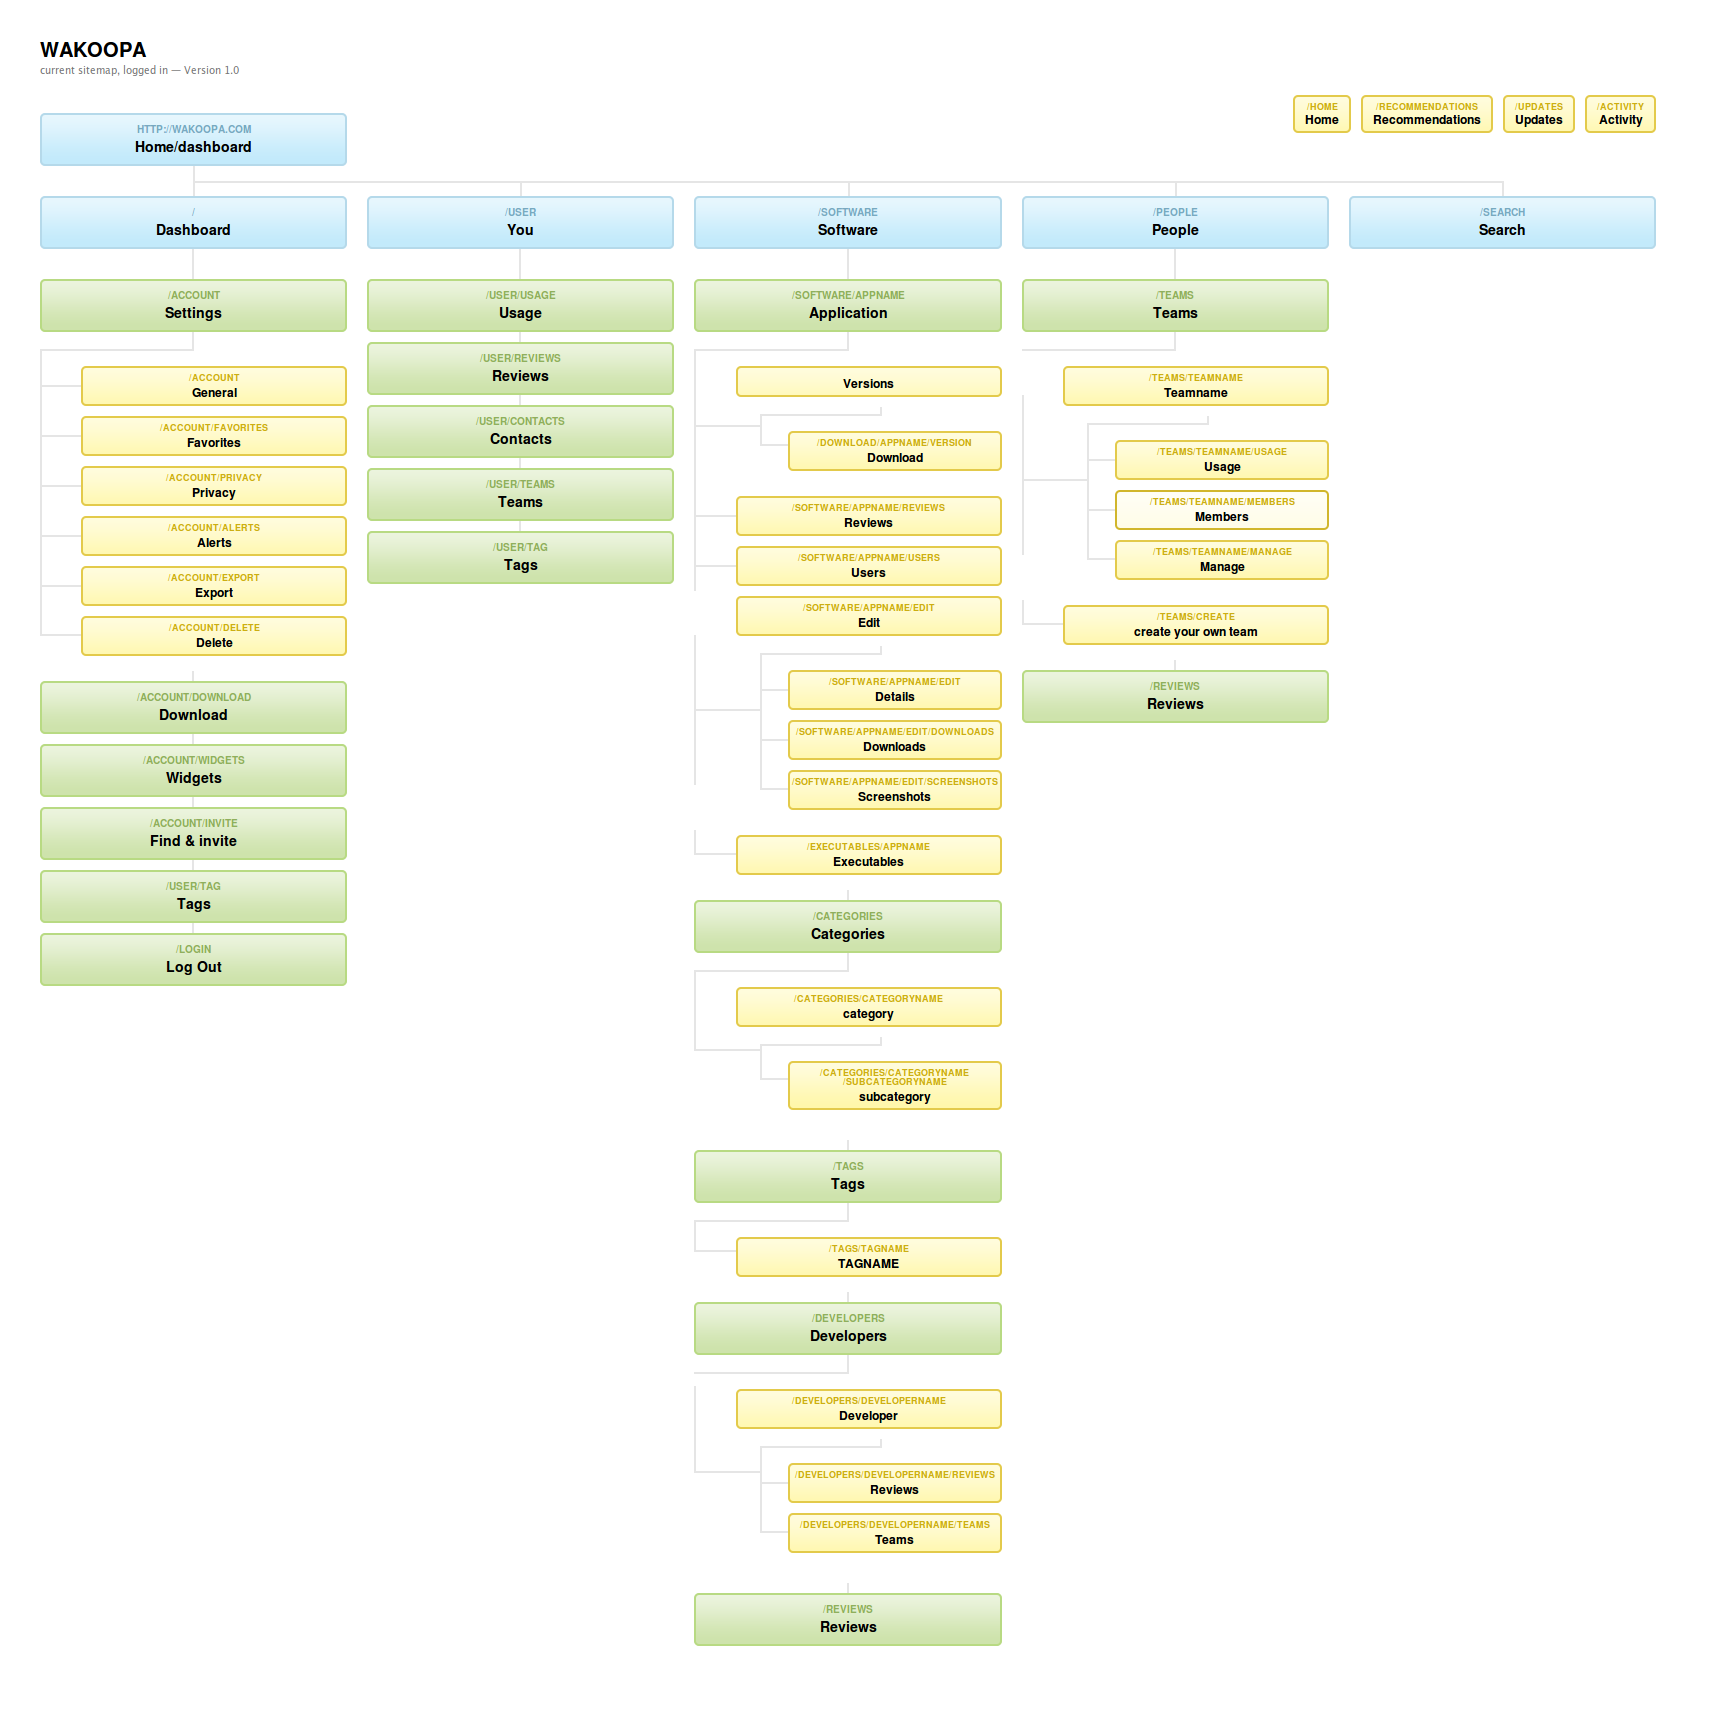
\includegraphics[width=\textwidth]{../images/currentnav}
      \end{center}
    \end{figure}

    \begin{figure}
      \begin{center}
      \caption{Verbeterde navigatie volgens \cite{Hoekman2008}}
        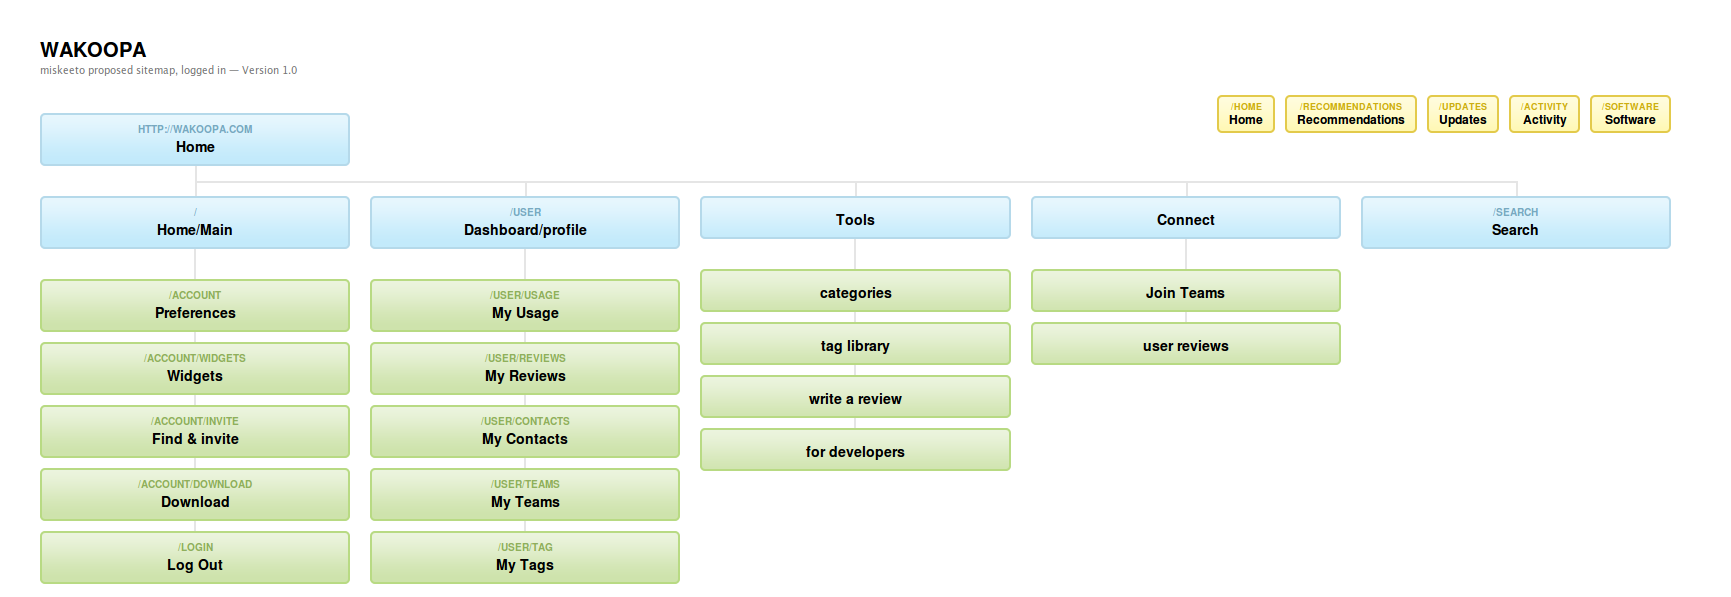
\includegraphics[width=\textwidth]{../images/miskeetonav}
      \label{miskeetonav2}
      \end{center}
    \end{figure}

      \begin{figure}
      \begin{center}
      \caption{Verbeterde navigatie volgens Navigatie workshop}
        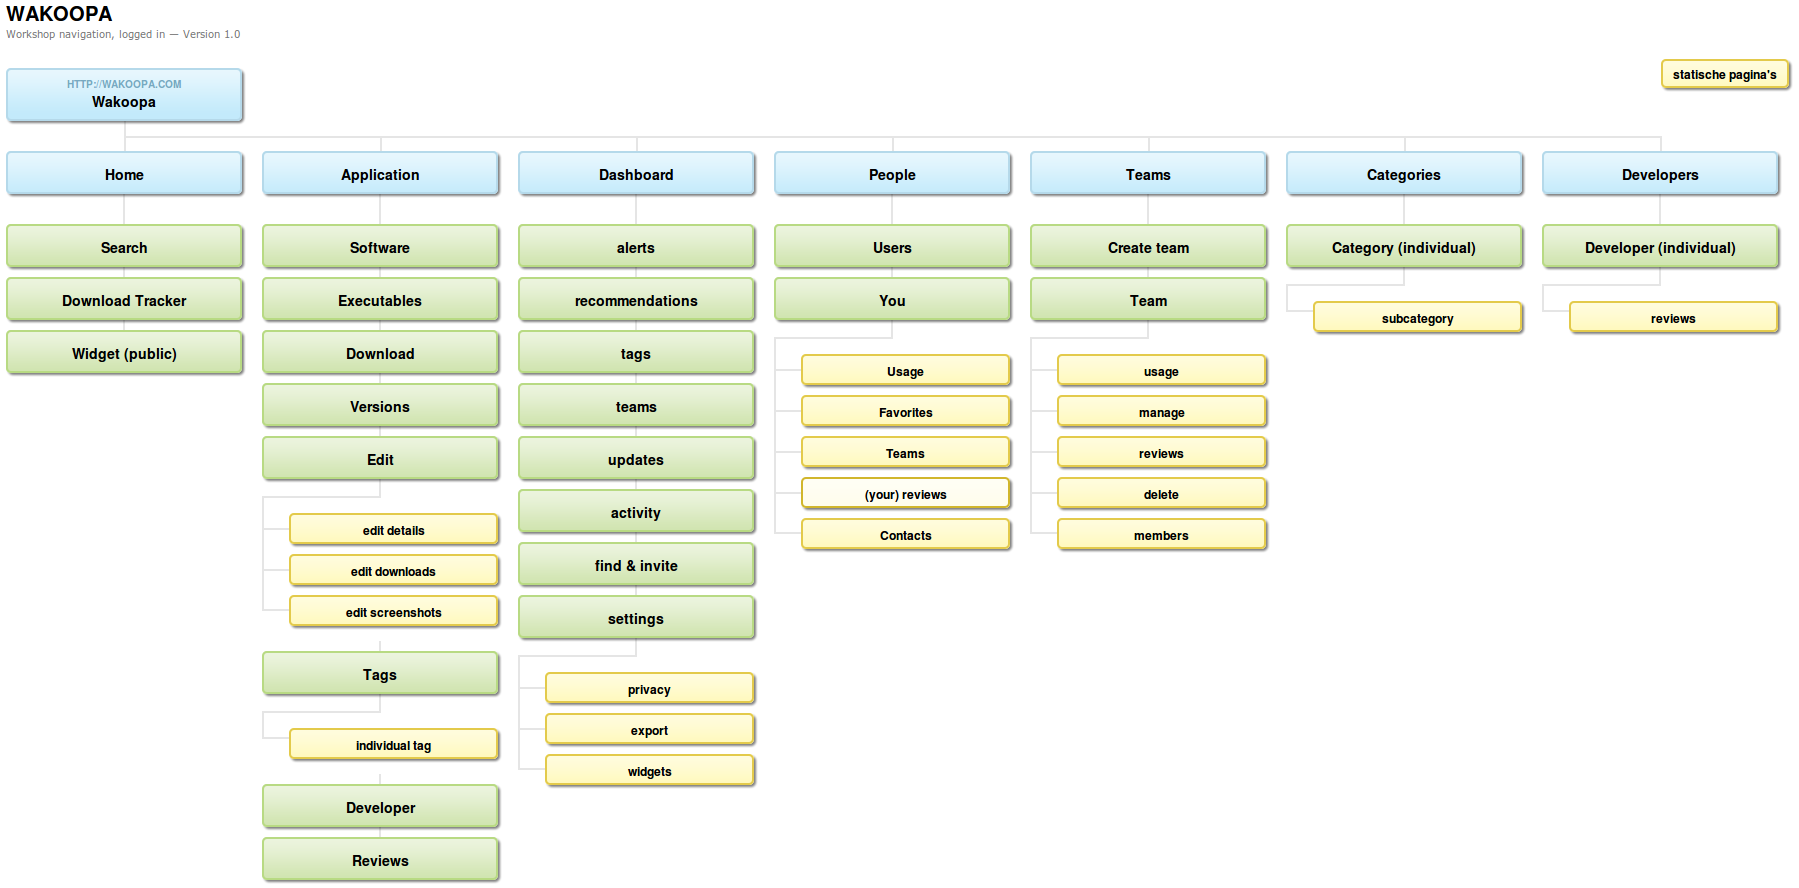
\includegraphics[width=\textwidth]{../images/workshopnav}
      \end{center}
    \end{figure}

    \begin{figure}
      \begin{center}
      \caption{Foto's van de workshop}
        \subfigure{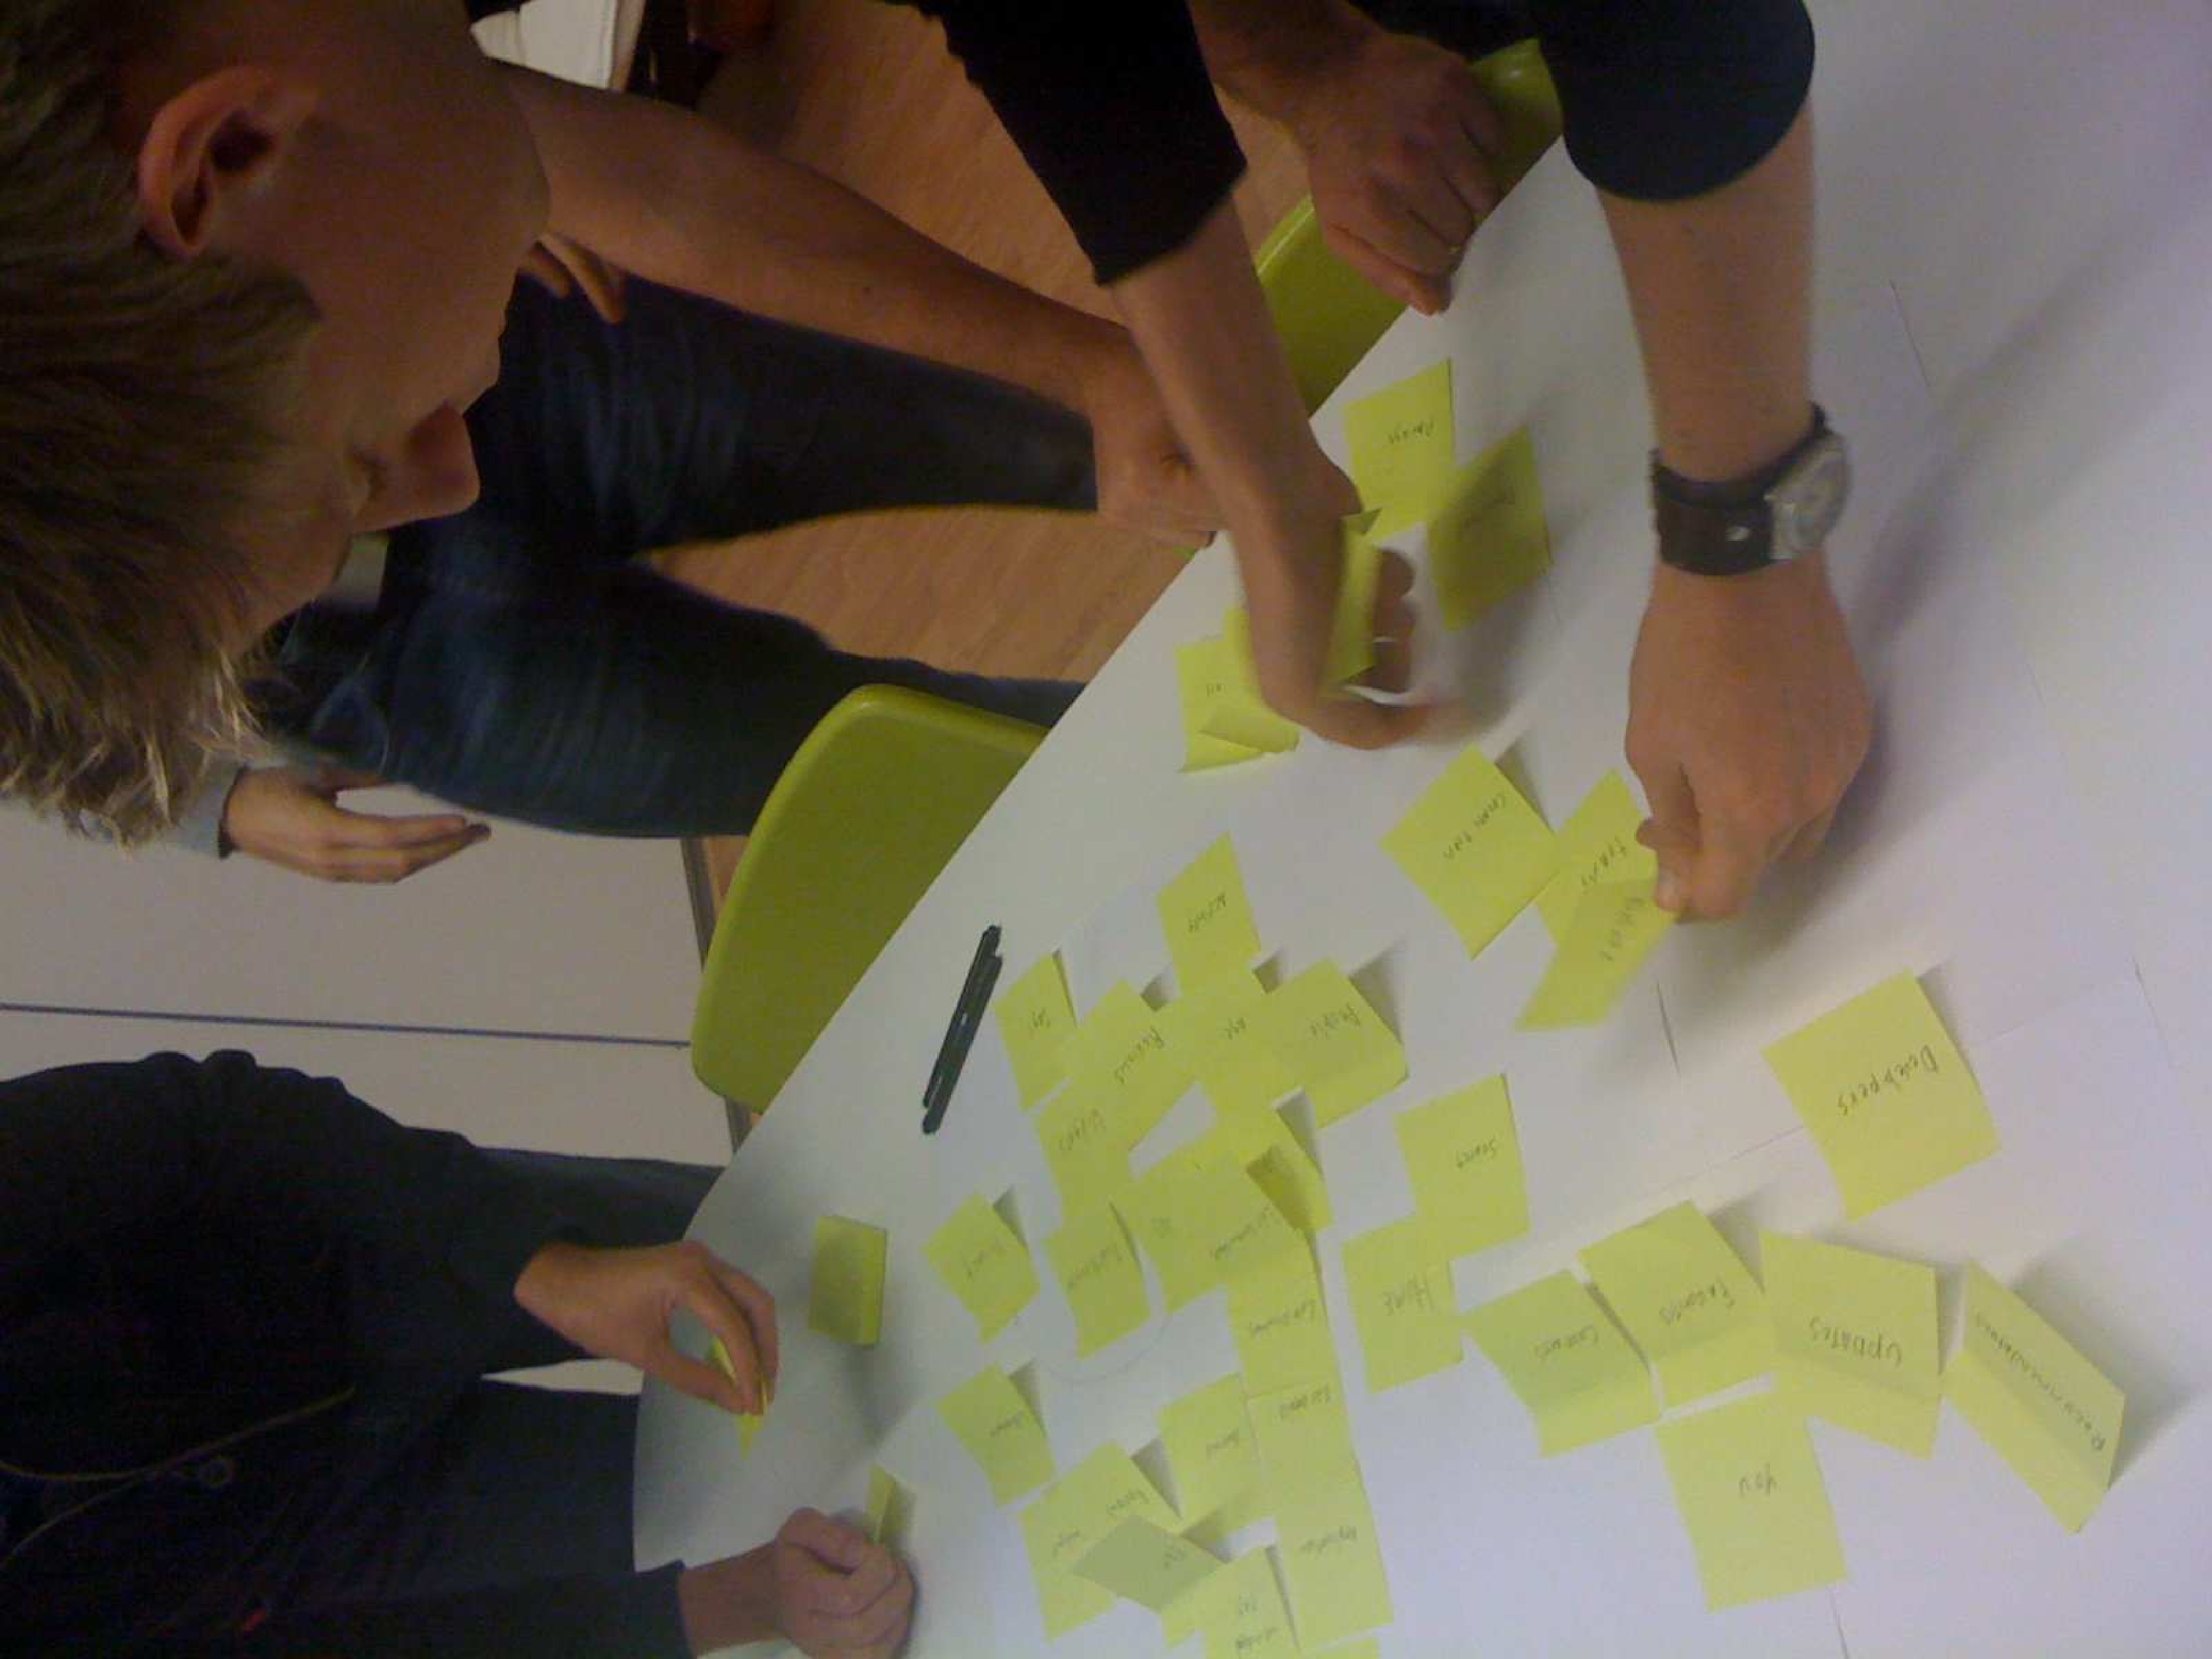
\includegraphics[height=6cm,angle=-90]{../images/navigatie-workshop/workshopimg1}}
        \subfigure{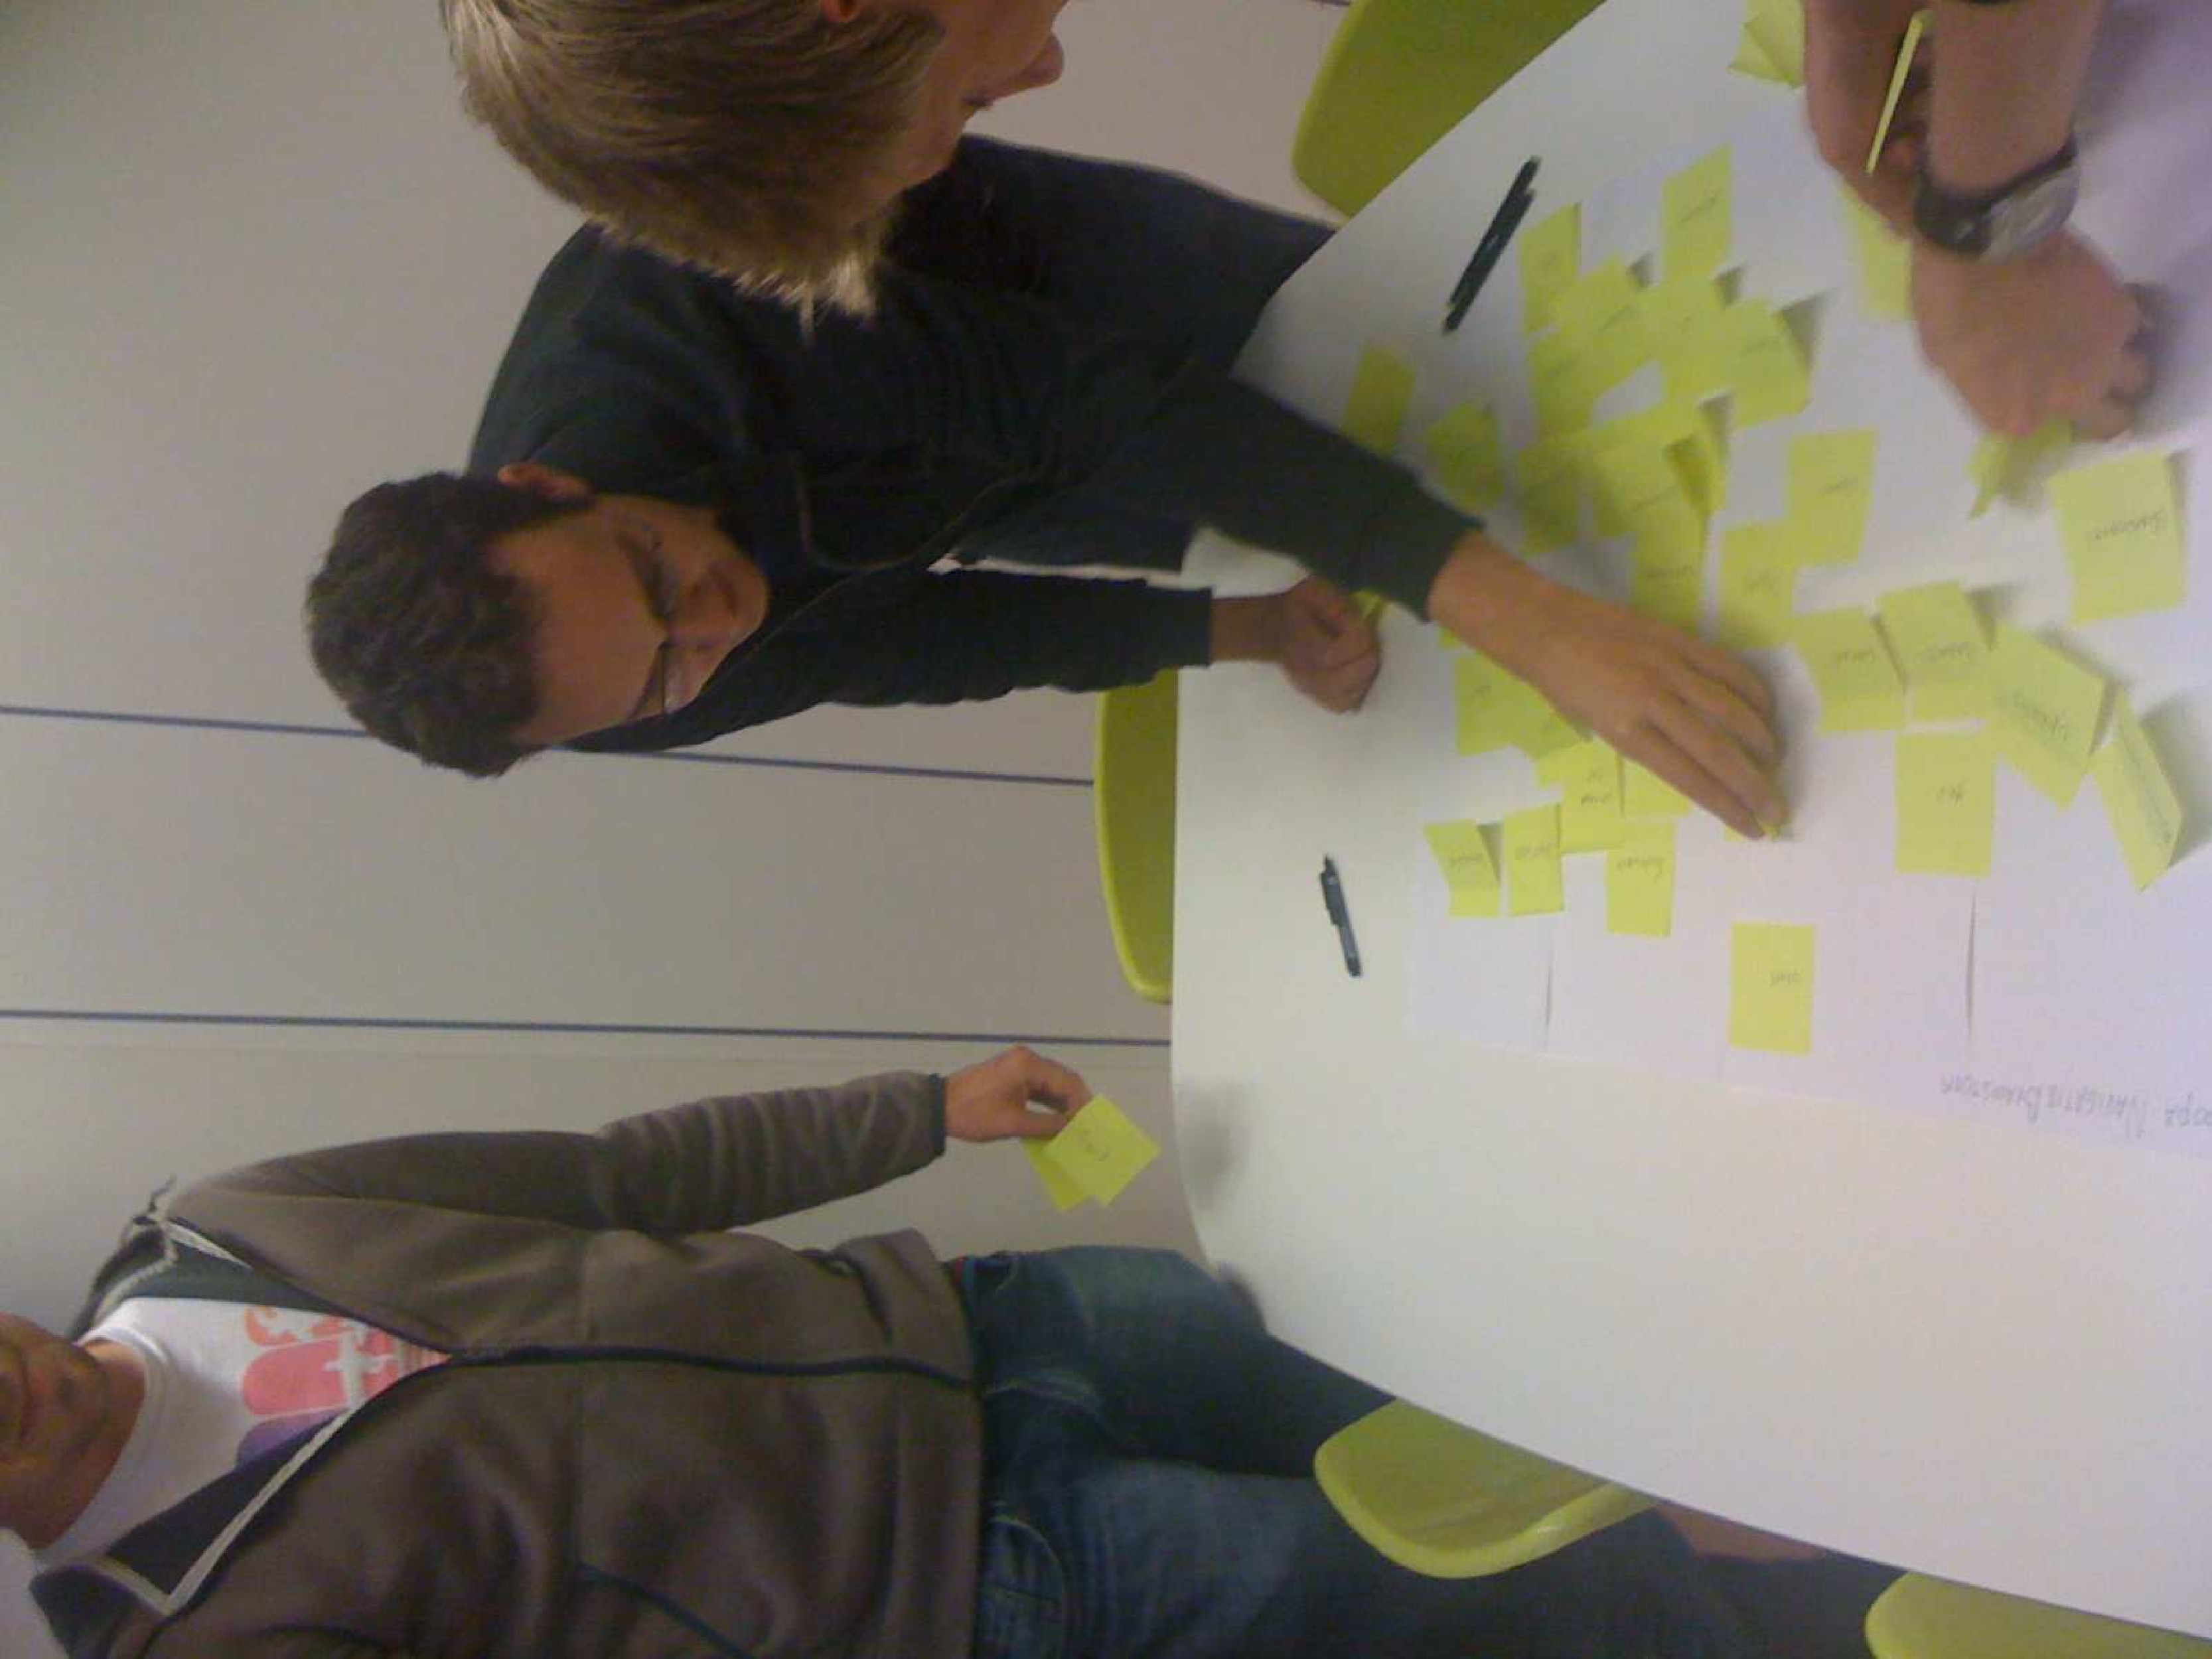
\includegraphics[height=6cm,angle=-90]{../images/navigatie-workshop/workshopimg3}}
        \subfigure{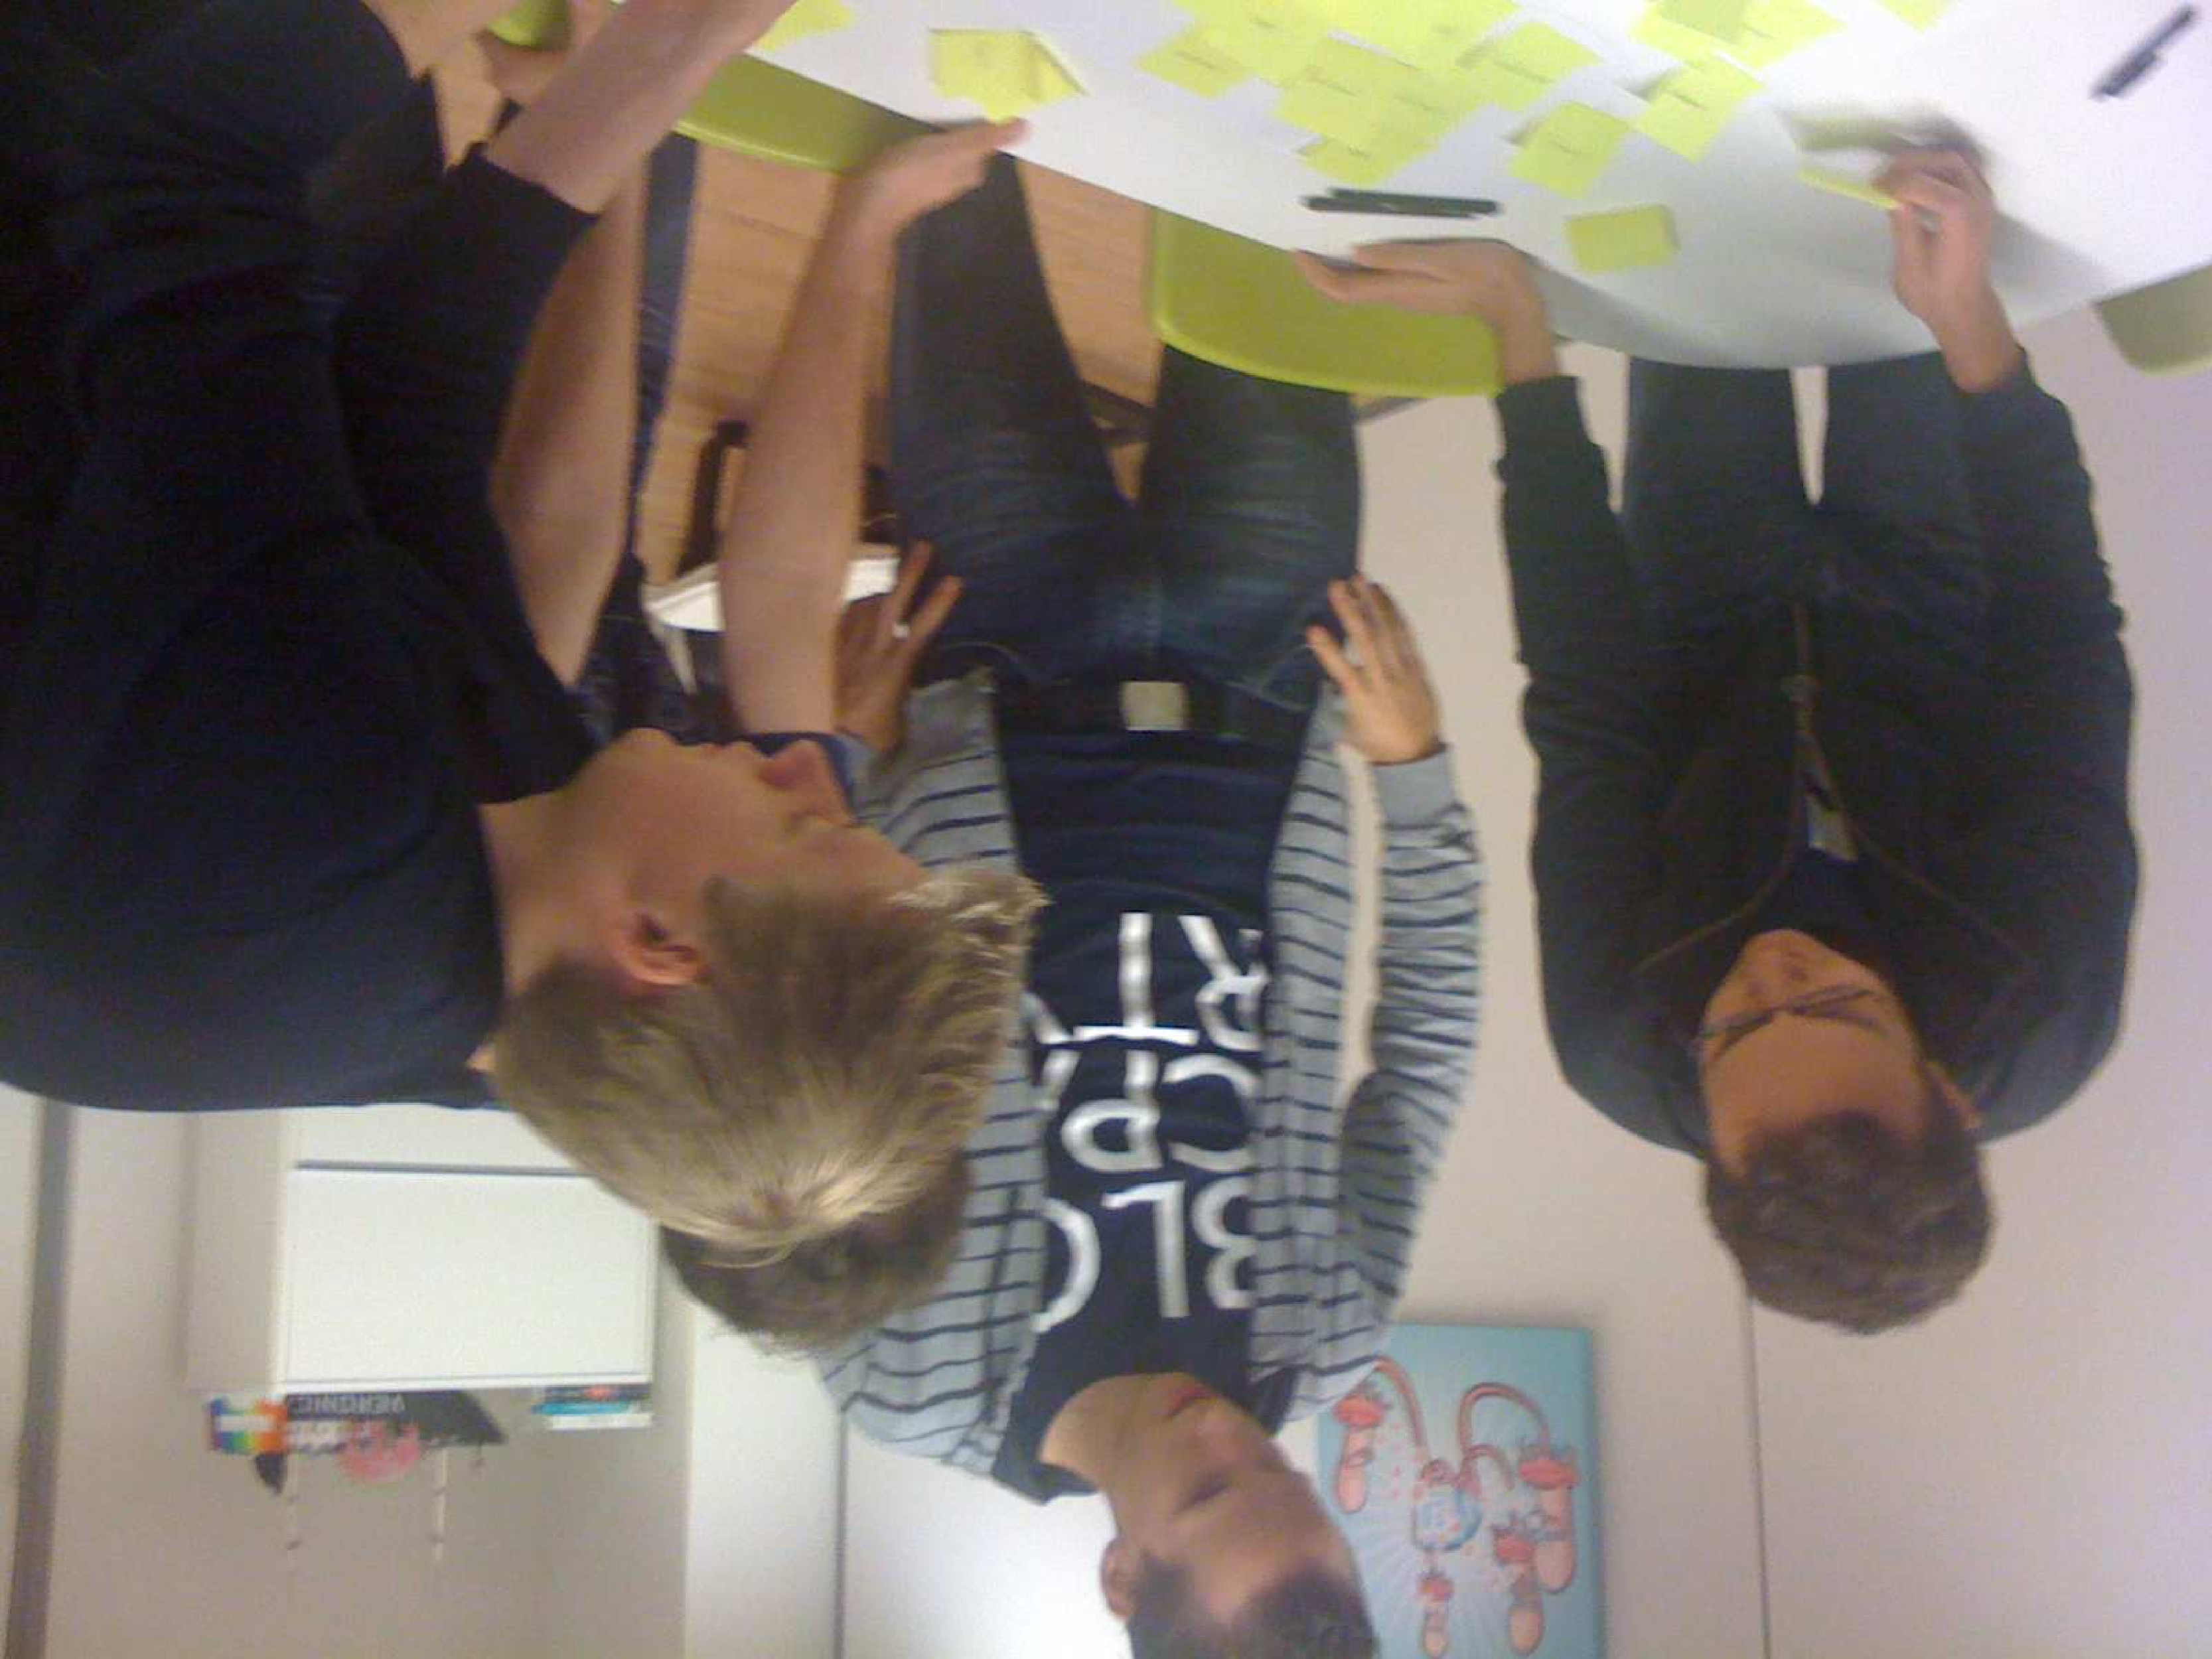
\includegraphics[height=4.5cm,angle=180]{../images/navigatie-workshop/workshopimg2}}
        \subfigure{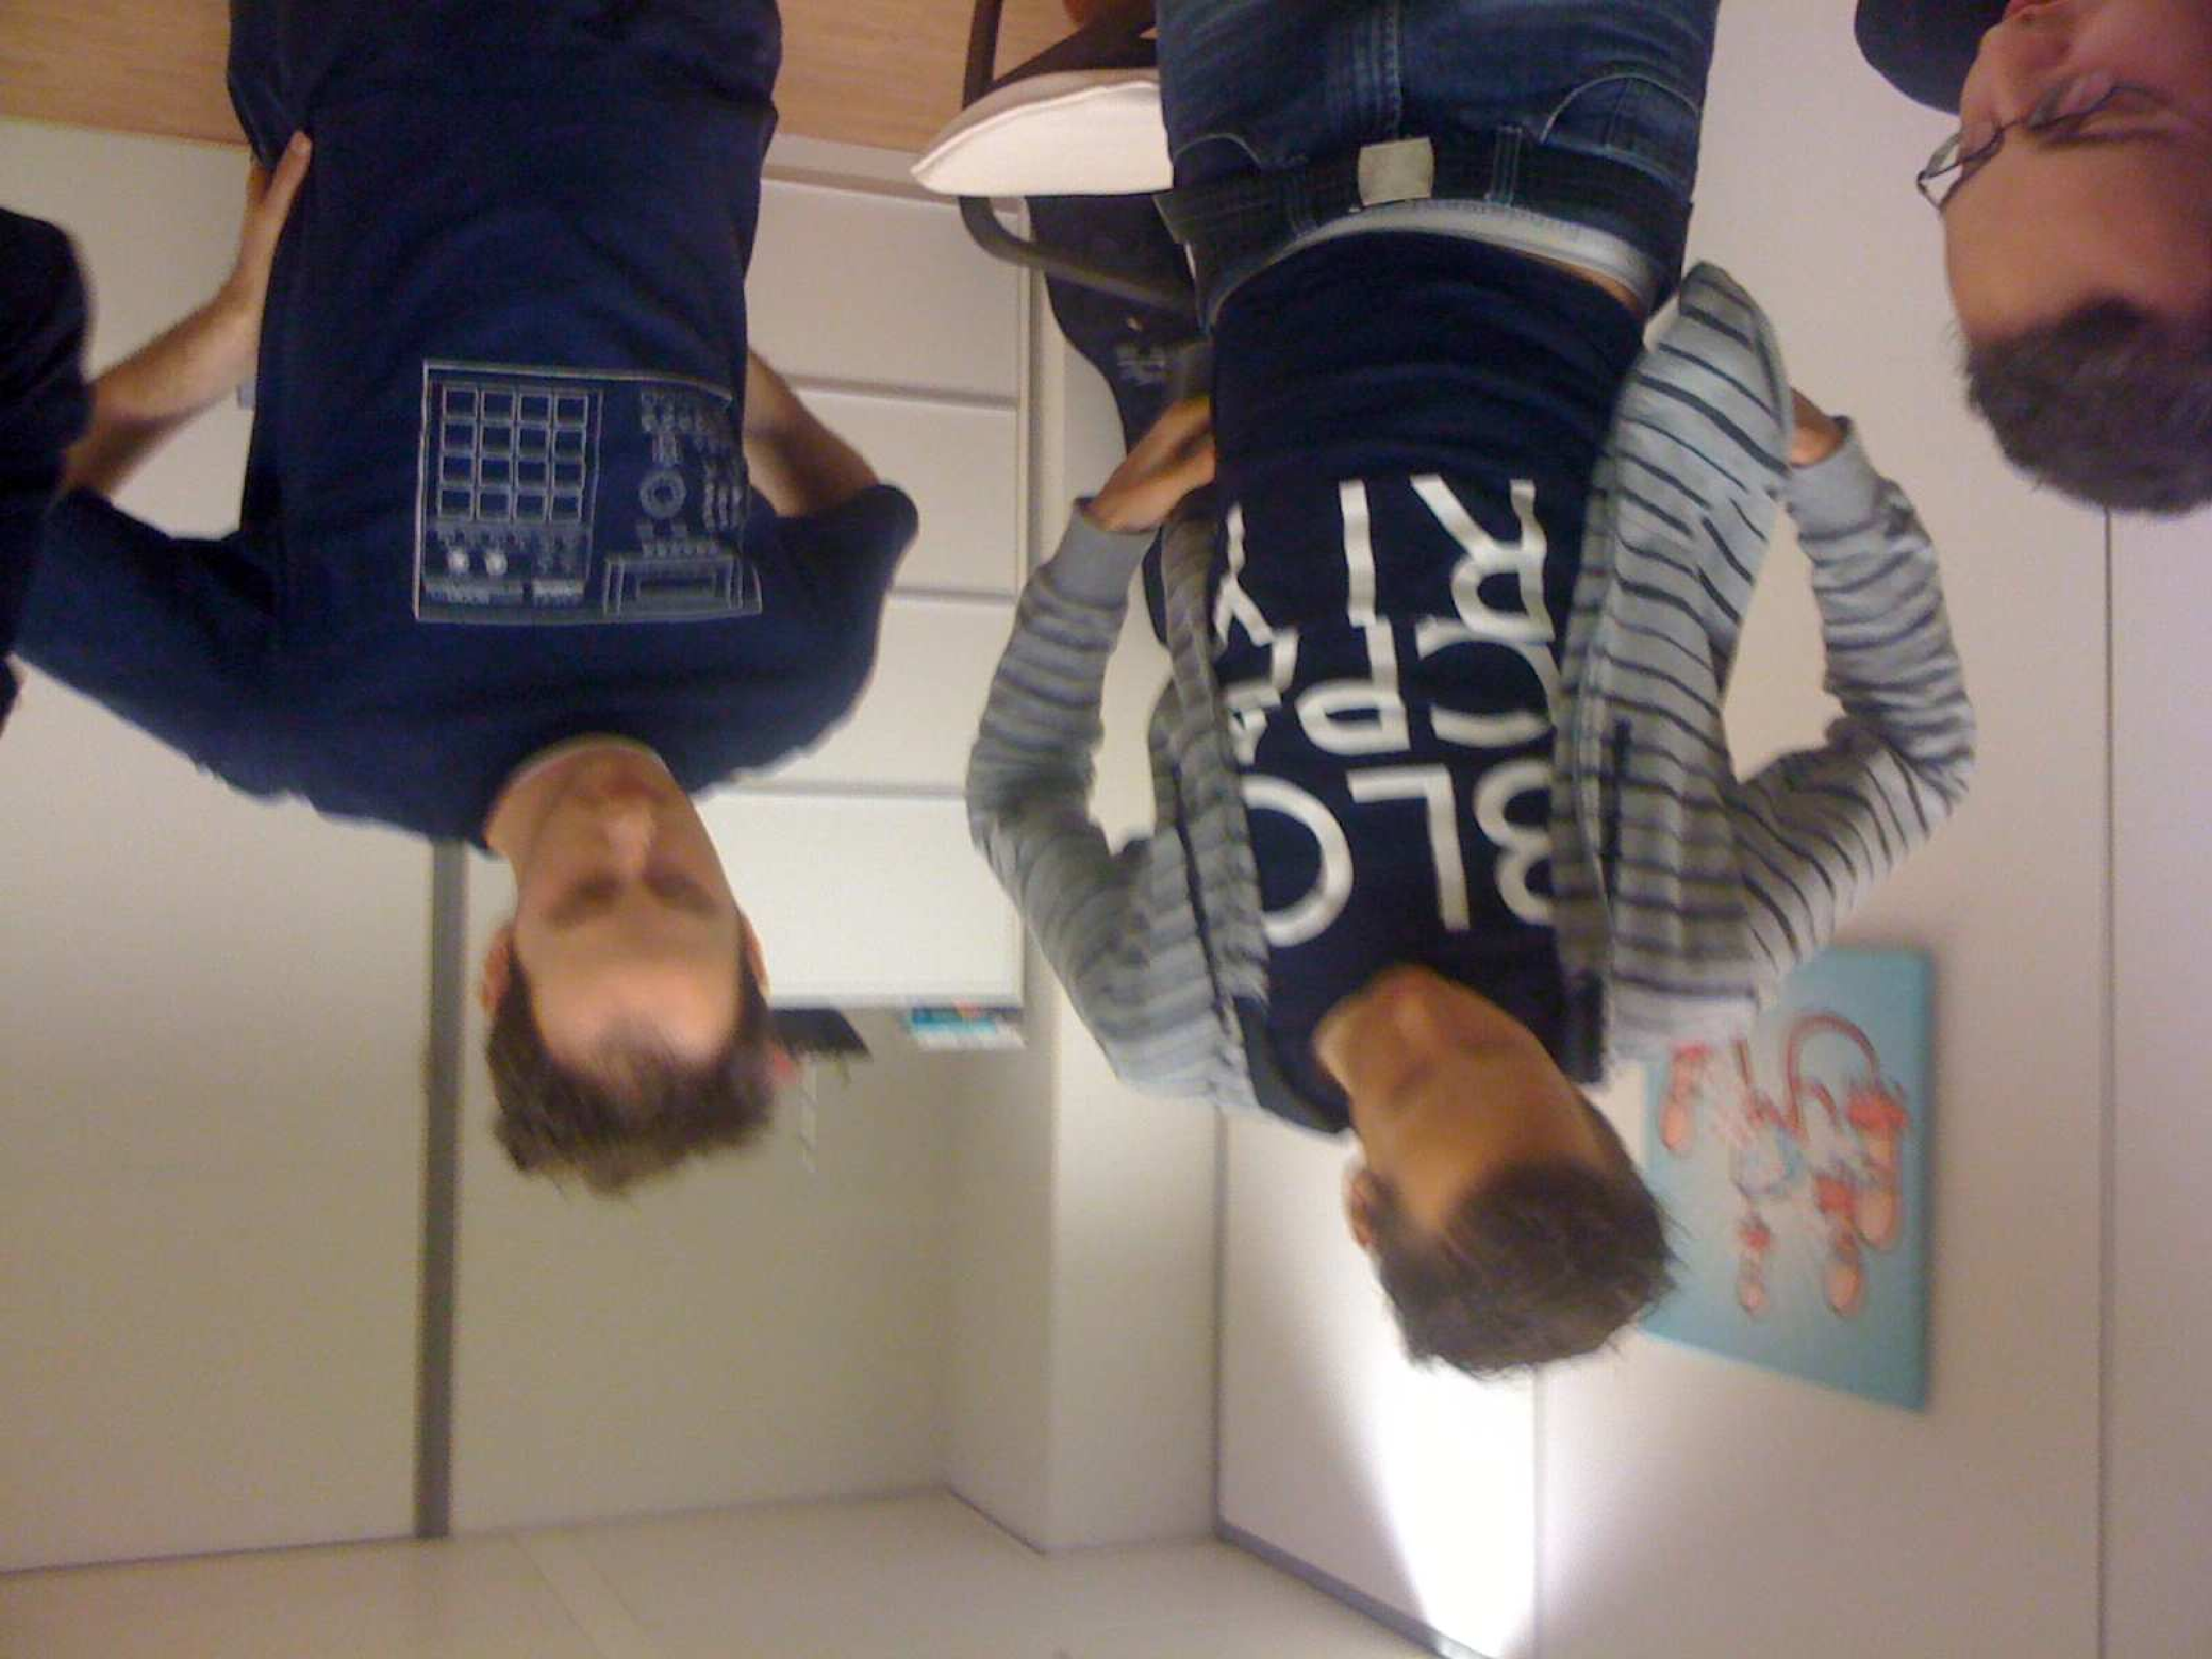
\includegraphics[height=4.5cm,angle=180]{../images/navigatie-workshop/workshopimg4}}
        \subfigure{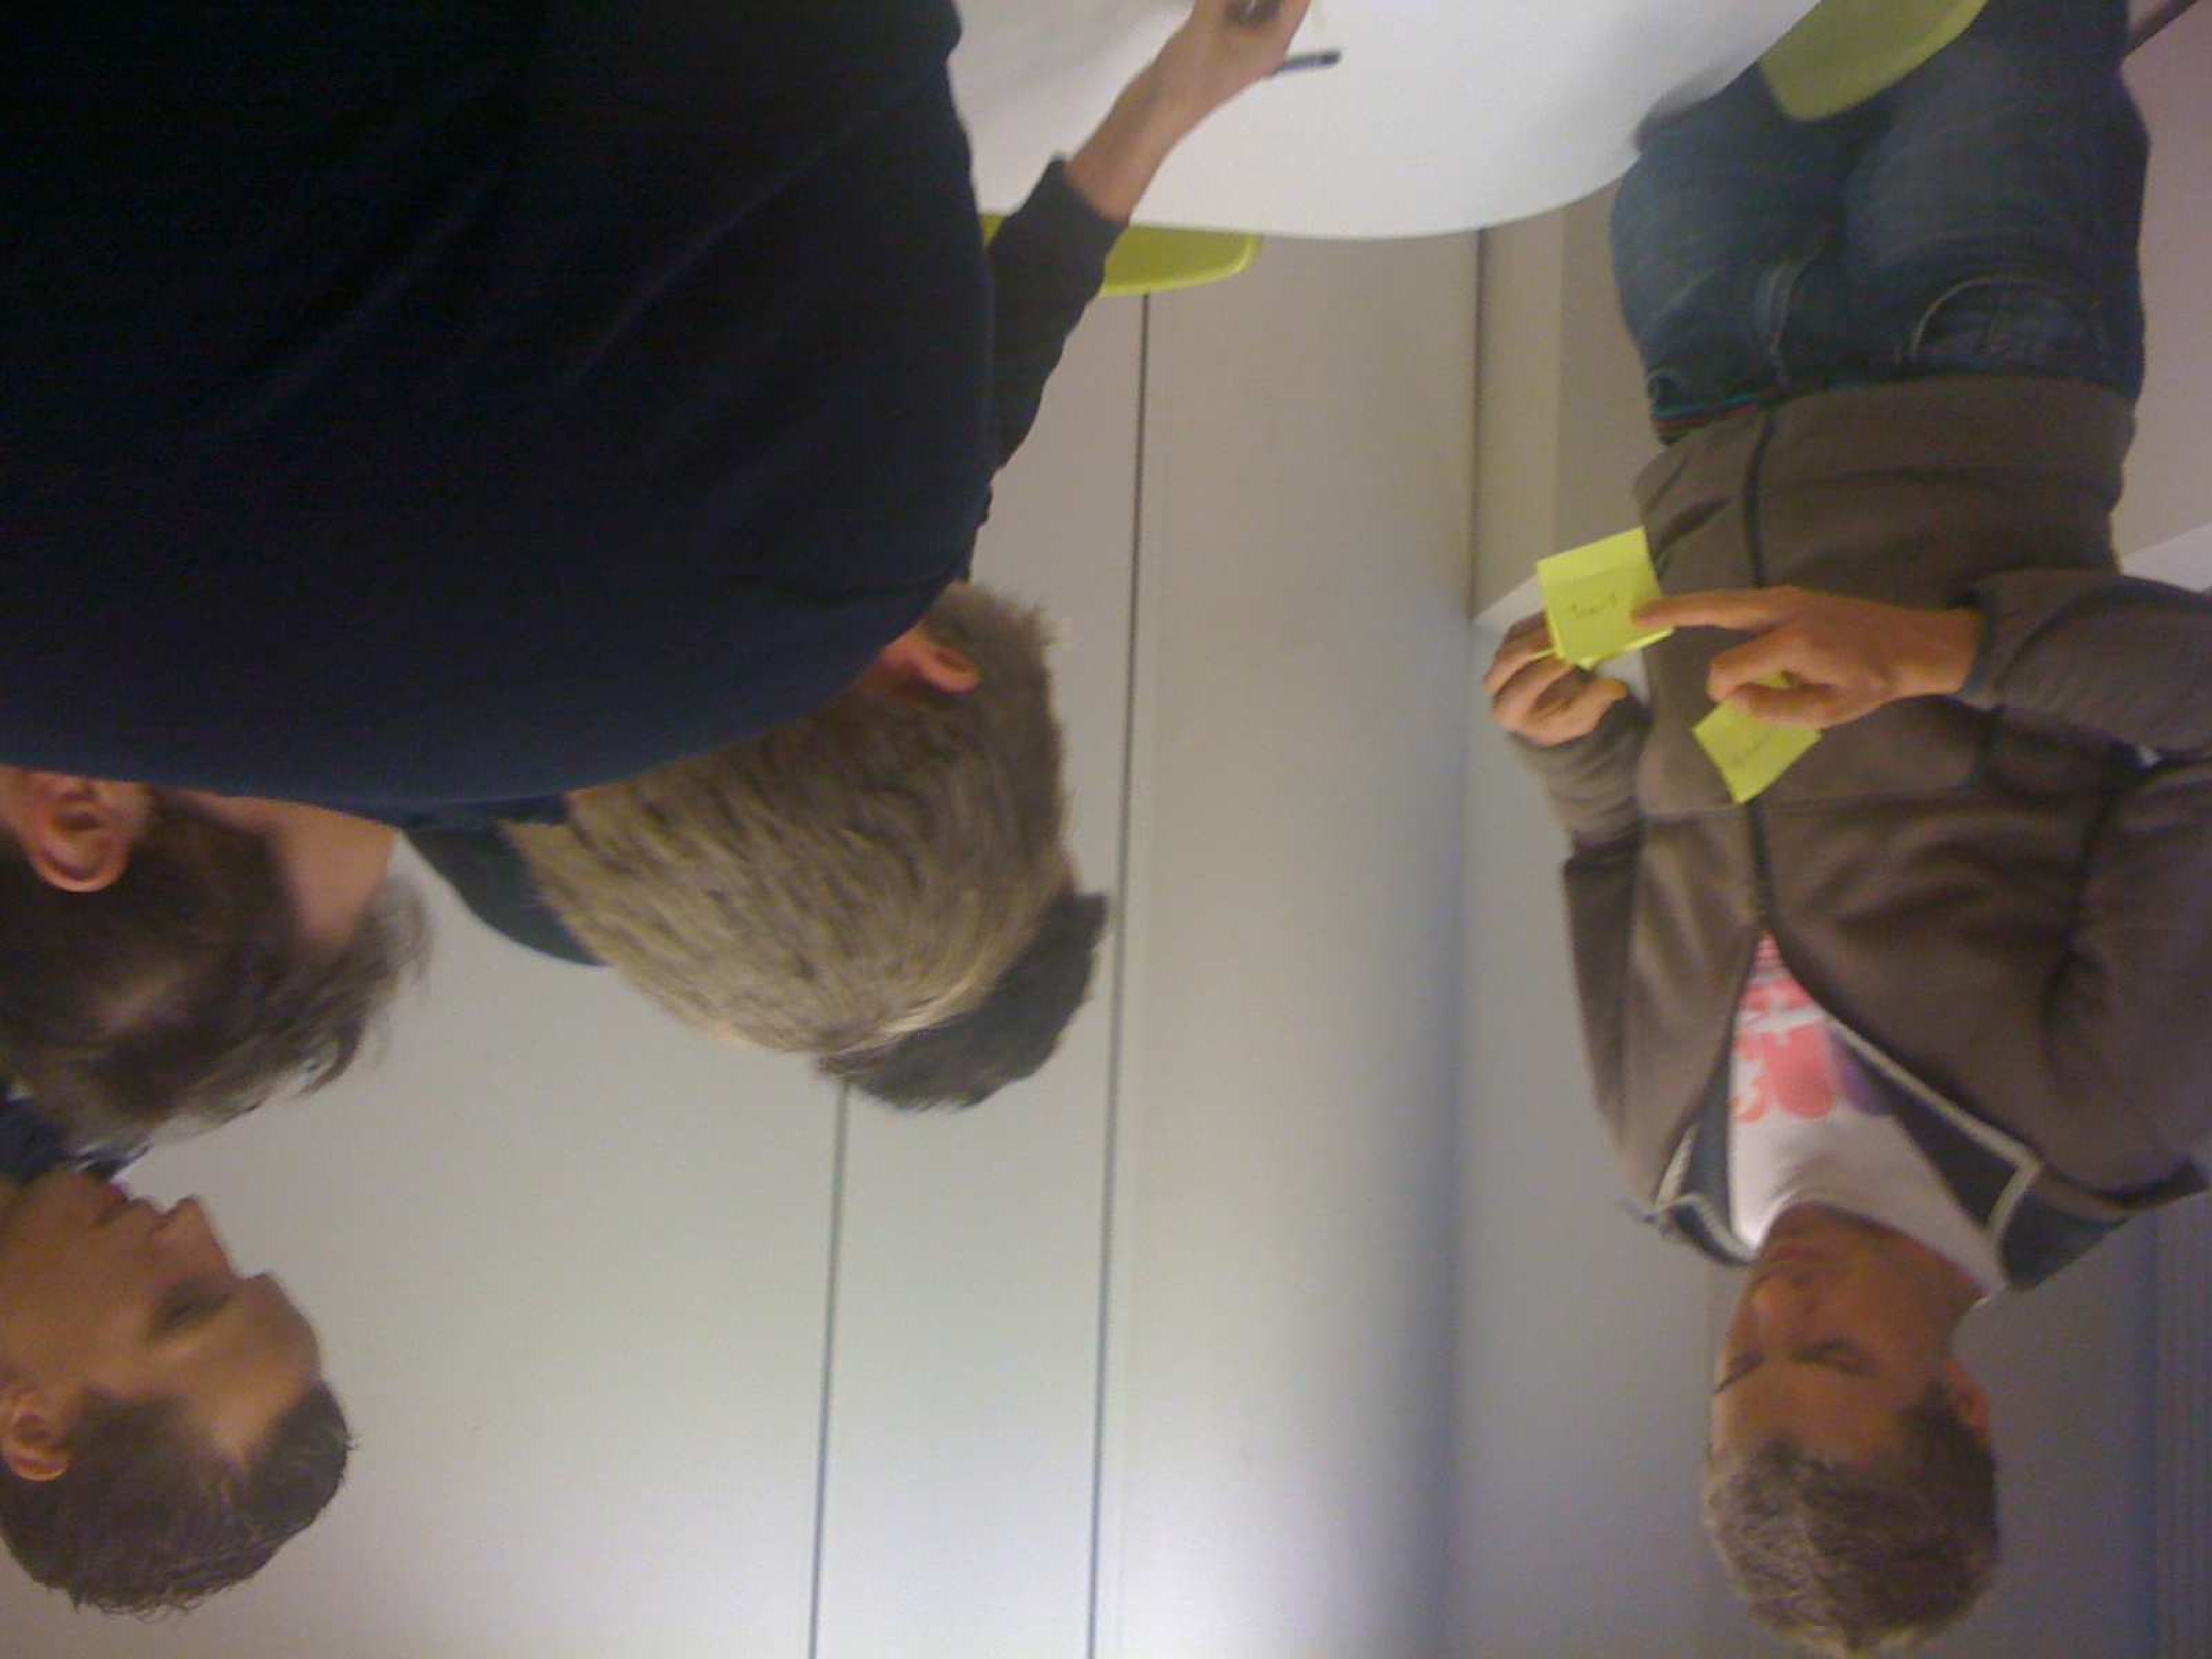
\includegraphics[height=4.5cm,angle=180]{../images/navigatie-workshop/workshopimg5}}
        \subfigure{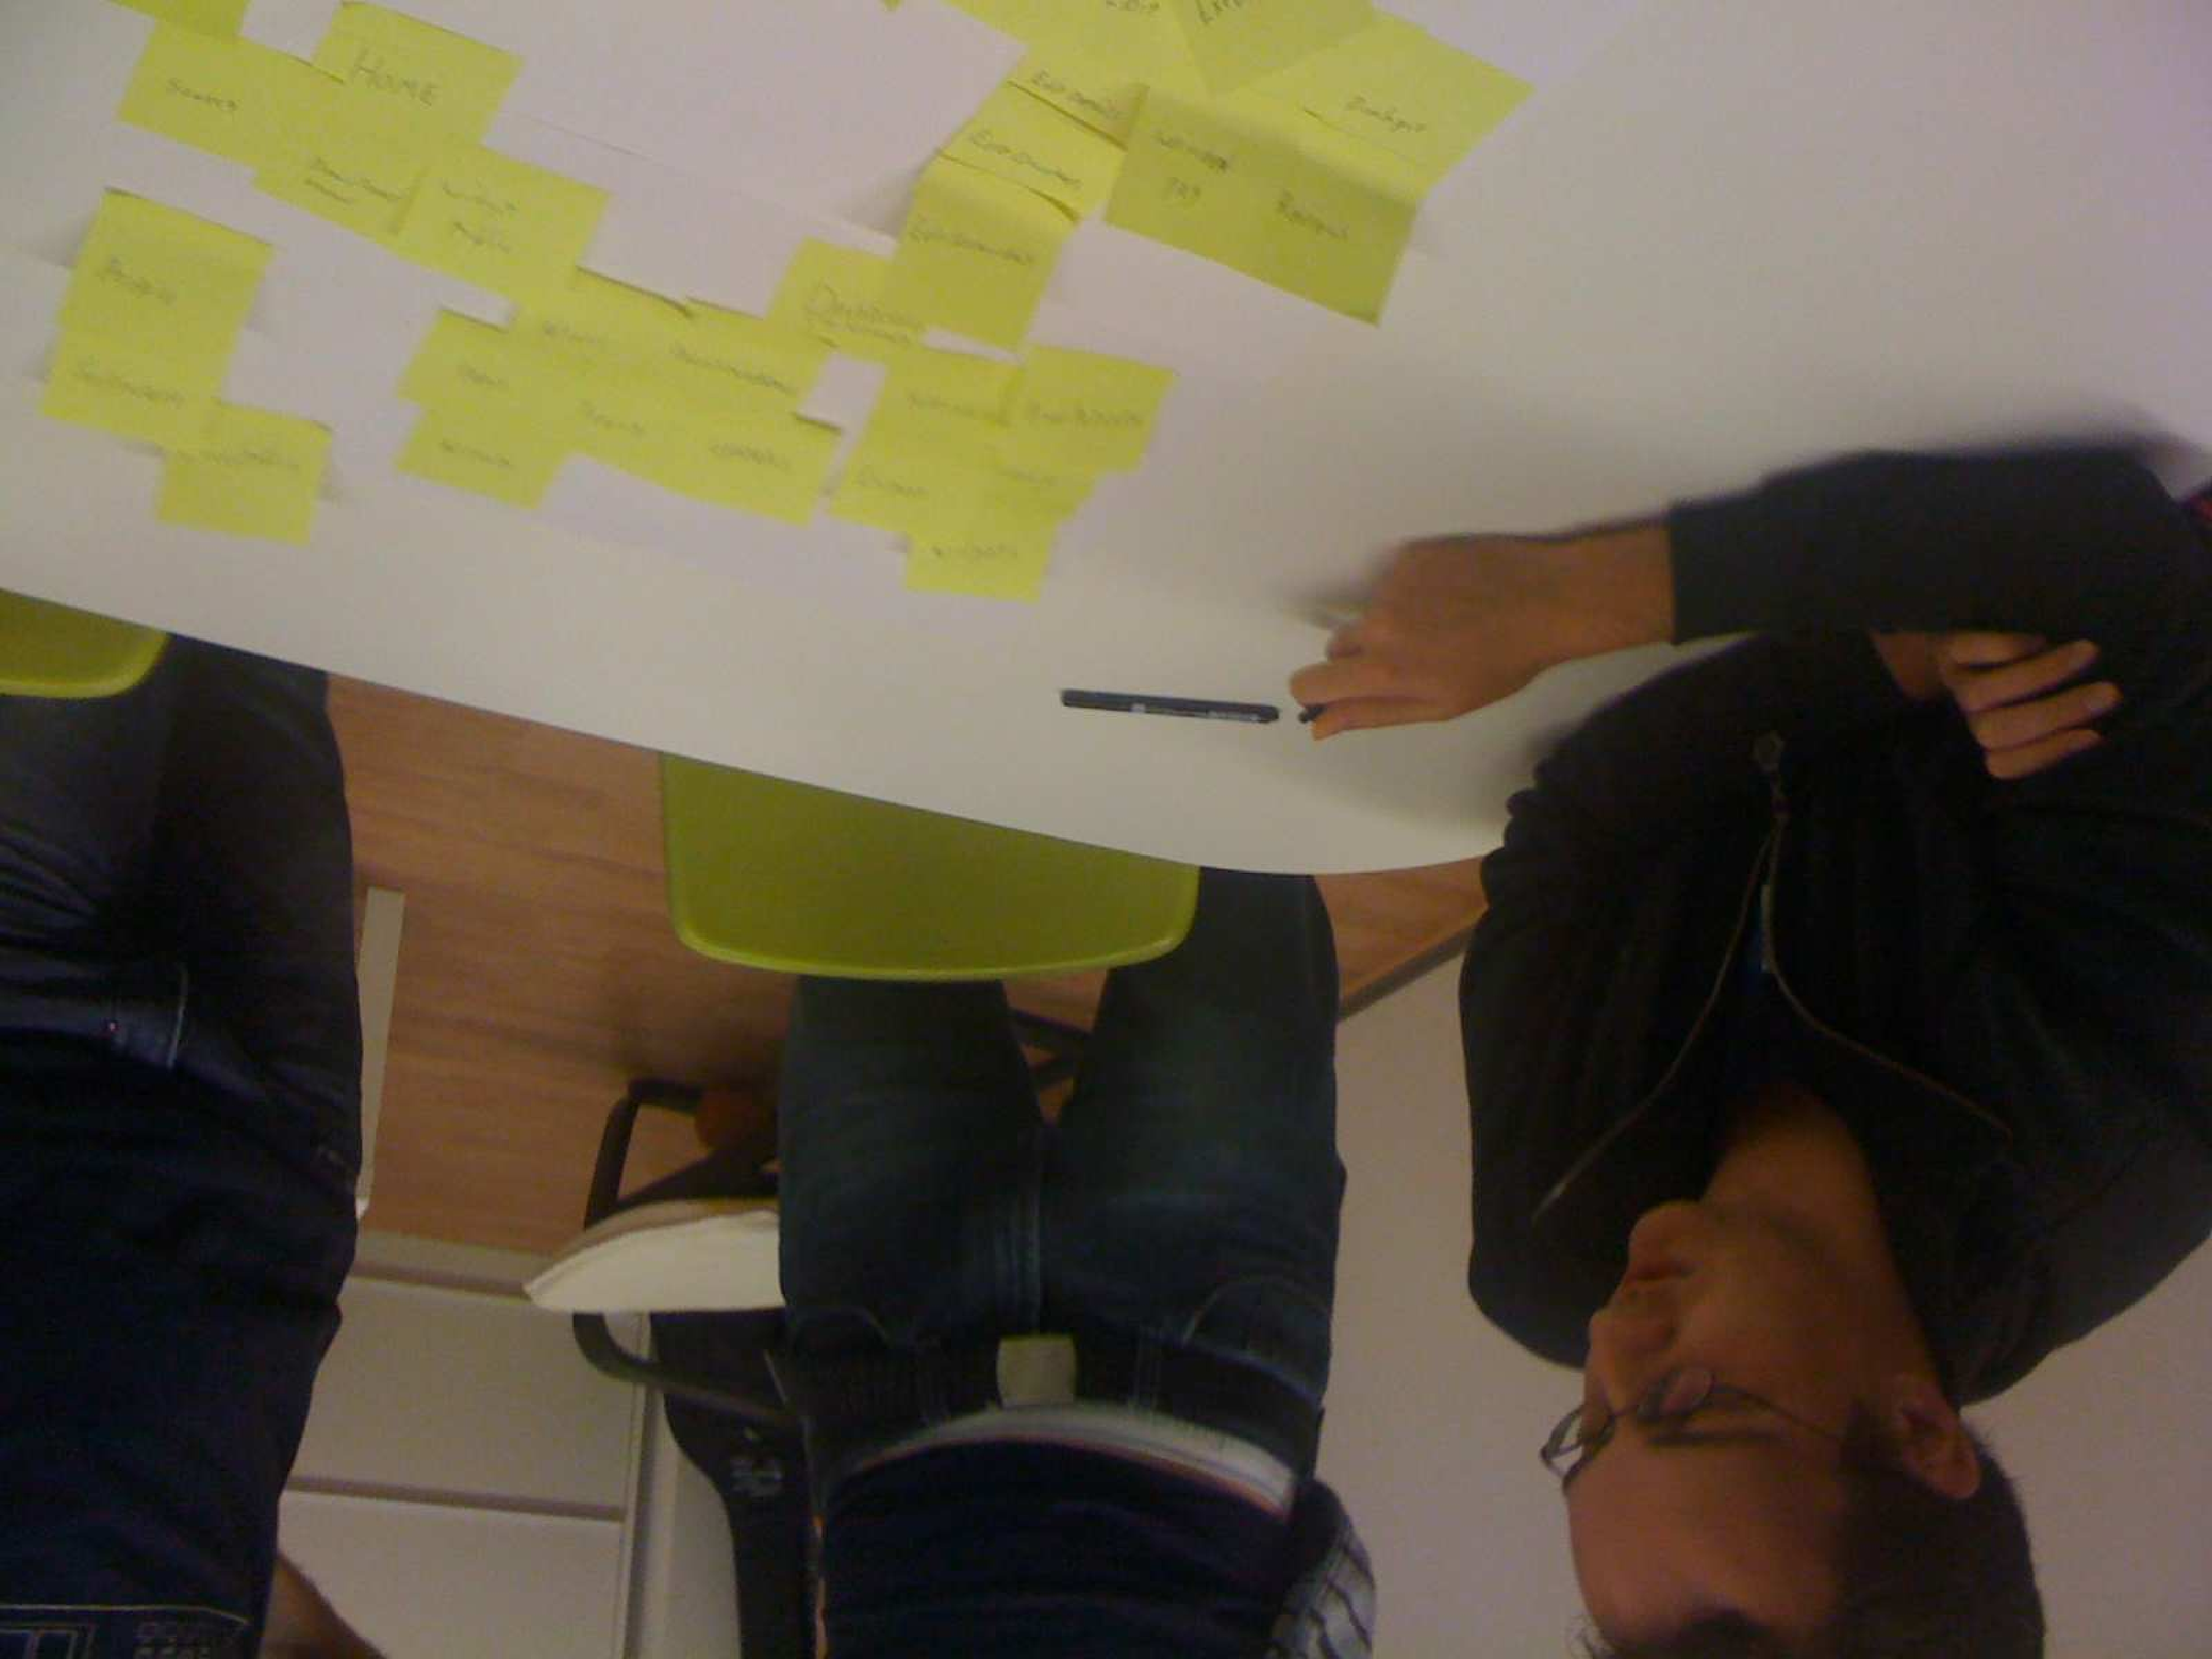
\includegraphics[height=4.5cm,angle=180]{../images/navigatie-workshop/workshopimg6}}
      \end{center}
    \end{figure}


    \label{navigationappendix}
  \chapter{Custom tracking items}
    \label{customtrackingappendix}
     De volgende items zullen worden getracked:
     \begin{itemize}
     \item vergroten van een screenshot
     \item bekijken van de category graph, periode dag
     \item bekijken van de category graph, periode week
     \item bekijken van de category graph, periode maand
     \item bekijken van de most used graph, periode dag
     \item bekijken van de most used graph, periode week
     \item bekijken van de most used graph, periode maand
     \item openen van de redenatie voor een aanbeveling
     \item het verwijderen van een aanbeveling
     \item het schrijven van een review
     \item zoeken via een ajax zoekveld
     \item openen van het favorite-toevoegen blok op een softwarepagina
     \item toevoegen van een favorite
     \item scrollen door gebruikers op een softwarepagina
     \item scrollen door screenshots op een softwarepagina
     \item openen van het tag-toevoegen blok op een softwarepagina
     \item toevoegen van een tag
     \item iemand toevoegen als contact
     \item verwijderen van een favorite
     \item openen van het privacy-settins blok op een softwarepagina
     \item verbergen van de intro promobar
     \item verzenden van een bericht via een reply
     \item verbergen van de promobar
     \item verbergen van de profile-completion bar
     \item laten zien van de software editing guidelines
     \end{itemize}


    \label{customtrackingappendix}
  \chapter{Enqu\^ete}
      \section{Demografie}
        Om te kijken in hoeverre de enqu\^ete de mening van alle Wakoopa leden vertegenwoordigd, is het belangrijk om te kijken of de demografie van de twee overeenkomen.De demografie van de respondenten is te vinden in figuren \ref{fig:gender}, \ref{fig:country} en \ref{fig:age}. Qua leeftijd, geslacht en land verschilt dit slechts een aantal procenten met de demografie van Wakoopagebruikers. De enqu\^ete, met 1069 respondenten, is daarom een goede graadmeter van de mening van Wakoopaleden.
        \begin{figure}
          \begin{center}
          \caption{Geslacht van respondenten}
            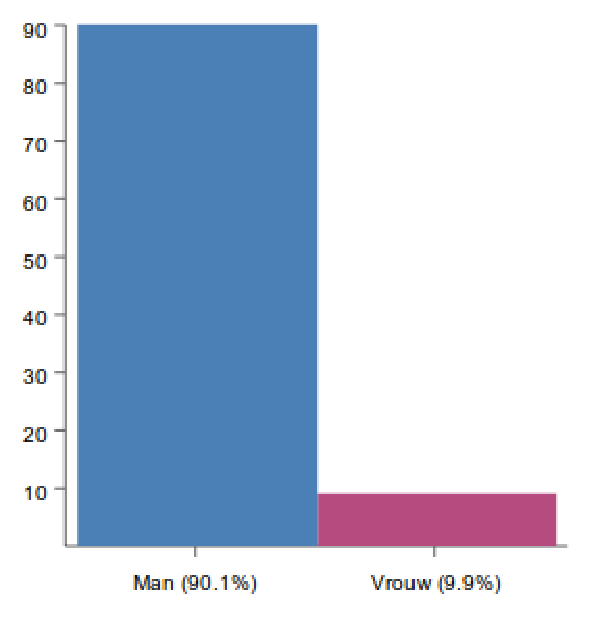
\includegraphics[height=60mm, angle=90]{../images/enquete/gender}
          \label{fig:gender}

          \caption{Land van afkomst van respondenten}
            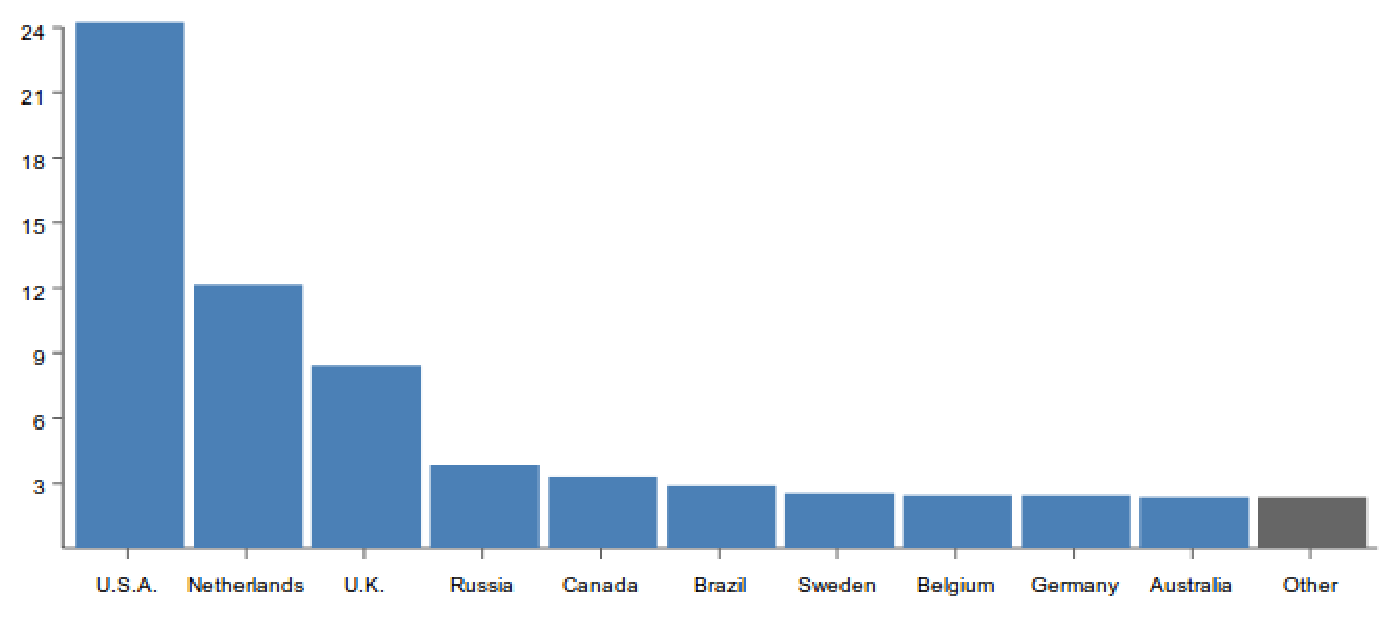
\includegraphics[height=60mm, angle=90]{../images/enquete/country}
            \label{fig:country}

          \end{center}
        \end{figure}

        \begin{figure}
          \begin{center}
          \caption{Leeftijd van respondenten}
            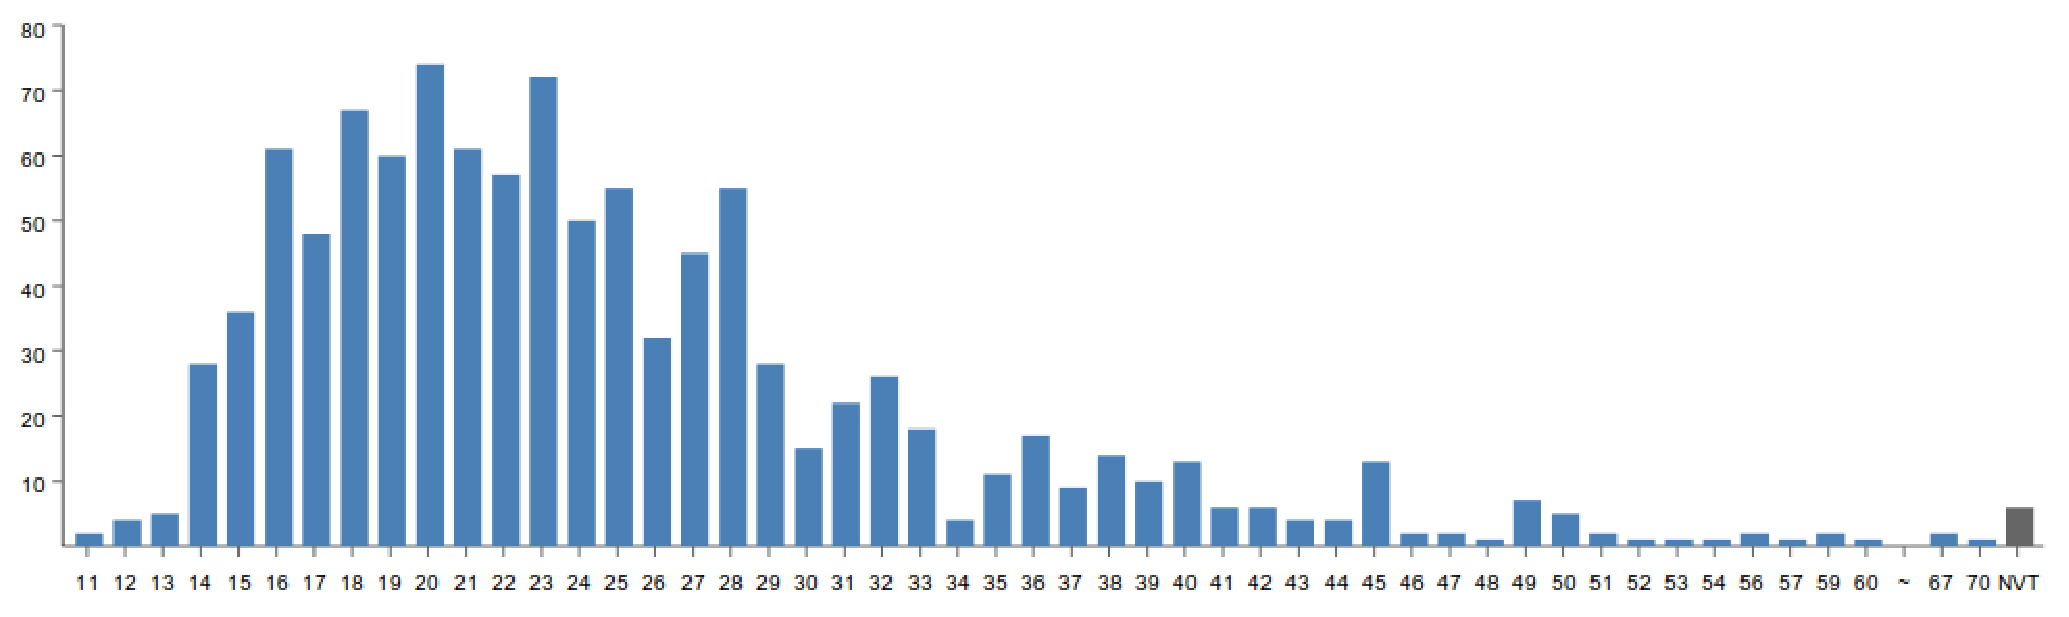
\includegraphics[height=58mm, angle=90]{../images/enquete/age}
          \label{fig:age}

          \end{center}
        \end{figure}

      \section{Bevindingen}
        De enqu\^ete ging verder met vragen naar hoe kundig de respondenten met computers waren (Figuur \ref{fig:skill}). Het overgrote deel (49.2\%) van de respondenten vind zichzelf \emph{excellent} op computergebied. een klein percentage vind zichzelf een novice (0.3\%) of classificeerd zichzelf als `lerende' (1.5\%). Eenentwintig procent acht zichzelf in het midden met `pretty good'. Als laatste is achtentwintig procent van de respondenten zelf actief bezig met het ontwikkelen van applicaties. Uit deze uitkomst is op te maken dat zich onder de respondenten een hoog percentage experts, of zogenaamde "power users", bevinden.
        \begin{figure}
          \begin{center}
          \caption{Kundigheid met computers}
            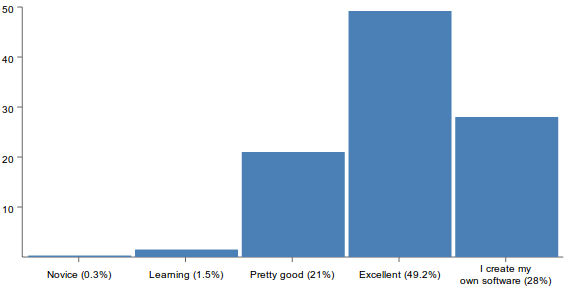
\includegraphics[height=50mm]{../images/enquete/good-with-computers}
          \label{fig:skill}
          \end{center}
        \end{figure}

      In Figuur \ref{fig:visit-website} werd de vraag gestelt hoe vaak gebruikers de Wakoopa site bezochten en er werd gevraagd waarom ze met dit interval de site bekeken. Het overgrote deel van de respondenten bekeek, met 43.1\%, de site wekelijks, gevolgd door een derde van de respondenten die dagelijks keek. Een greep uit de gegeven redenen:
        \begin{figure}
          \begin{center}
          \caption{Hoe vaak wordt de website bezocht?}
            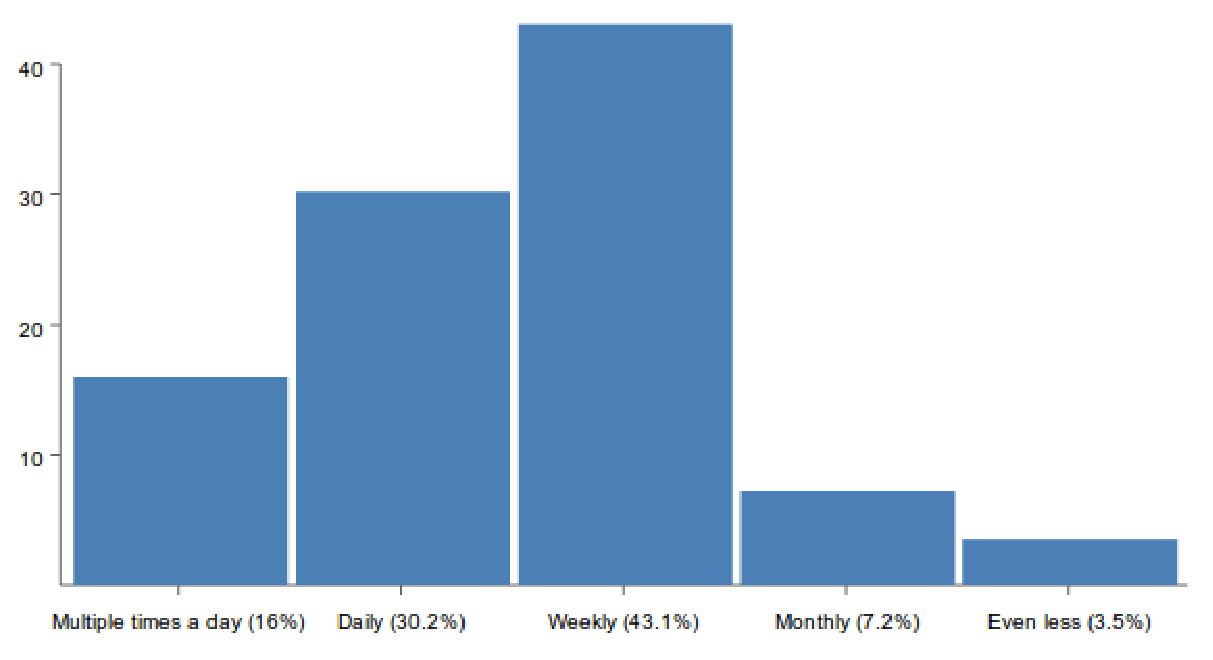
\includegraphics[height=50mm]{../images/enquete/visit-website}
          \label{fig:visit-website}
          \end{center}
        \end{figure}

      \paragraph{Wekelijk (43.1\%)}
        \begin{itemize}
          \item Because of the weekly summary mail
          \item Because that is when I get my summary
          \item I need some weekly reports about my software and timetracking reports.
          \item To see the "big" changes is my software behaviour. And to see if there is new software i could try out.
        \end{itemize}

      \paragraph{Dagelijks (30.2\%)}
        \begin{itemize}
          \item It's interesting to see all the data and usage stuff.
          \item To check what level I am. Always seeking to level up..!
          \item To check out what new software is out there \& it's cool to see what my habits are on my Mac.
          \item Check my profile stats
        \end{itemize}

      \paragraph{Meerdere malen per dag (16\%)}
        \begin{itemize}
          \item To see how many points i'm earning, and to just snoop on other peoples profiles. you know, creep. like on facebook. but the people here are more interesting than my facebook people :)
          \item Well, the system tray icon keeps notifying me the new activities
          \item To see how my friends are doing and me, and so I can win in the battle of using the most software in less time. :)
          \item Because I love statistics, I find it rewarding to see figures and graphs about something I accomplished! that's the reason why I'm also a last.fm and whatpulse addict. and apart from that, I really like software (especially freeware) and like to see suggestions for other software.
        \end{itemize}

      \paragraph{Maandelijks (7.2\%)}
        \begin{itemize}
          \item There's no need to use it more often
          \item Because I got an update.
          \item I like to see my stats and get new ideas on software/sites.
          \item I only check the site when I am looking for alternative software or I see something I like in the newsletter.
        \end{itemize}

      \paragraph{Minder dan maandelijks (3.5\%)}
        \begin{itemize}
          \item I'm still waiting for the linux app
          \item Nothing of tons of interest on site, just as often as I visit Last.FM It is useful when uninstalling things.
          \item Because I use Linux, I am waiting for a Linux tracker. Without it, Wakoopa is just another computer-oriented forum to me.
        \end{itemize}

      \paragraph{}Zoals uit de verschillende gegeven redenen op te merken is, is er een relatie tussen hoe vaak mensen de site bezoeken en hoe enthousiast ze er over zijn. Onder wekelijkse bezoekers is het aantal wat aangeeft de website te bezoeken na het ontvangen van de wekelijkse mail het hoogst. De mensen die een of meerdere malen per dag de site bekijken, zijn er voornamelijk voor de grafieken, statistieken en punten. Omgekeerd, de respondenten die slechts maandelijks of minder de site bekijken, zeggen dat ze dit doen omdat er niet genoeg nieuws of informatie op de site staat om deze vaker te bezoeken.

        \begin{figure}
          \begin{center}
          \caption{over welke nieuwe functionaliteit ben je het meest enthousiast?}
            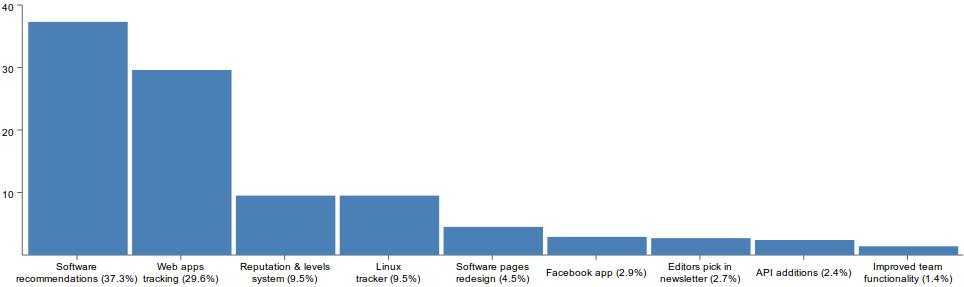
\includegraphics[width=\textwidth]{../images/enquete/recent-additions}
          \label{fig:enthousiast}
          \end{center}
        \end{figure}

      Een learning network is vaak bezig met het ontwikkelen en online plaatsen van nieuwe functionaliteit. Het belangrijk om bij te houden wat de impact hiervan op de gebruikers is. Om dit te onderzoeken vroegen we in figuur \ref{fig:enthousiast} aan de respondenten welke recente toevoeging ze het meest enthousiast over waren. Met 37.3\% zijn de respondenten het meest enthousiast over de software aanbevelingen, kort daarop gevolgd door het tracken van web apps met 29.6\%. De eerstvolgende zijn respectievelijk het level-systeem en de linux tracker met beide 9.5\%.

        \begin{figure}
          \begin{center}
          \caption{Waar komt Wakoopa tekort?}
            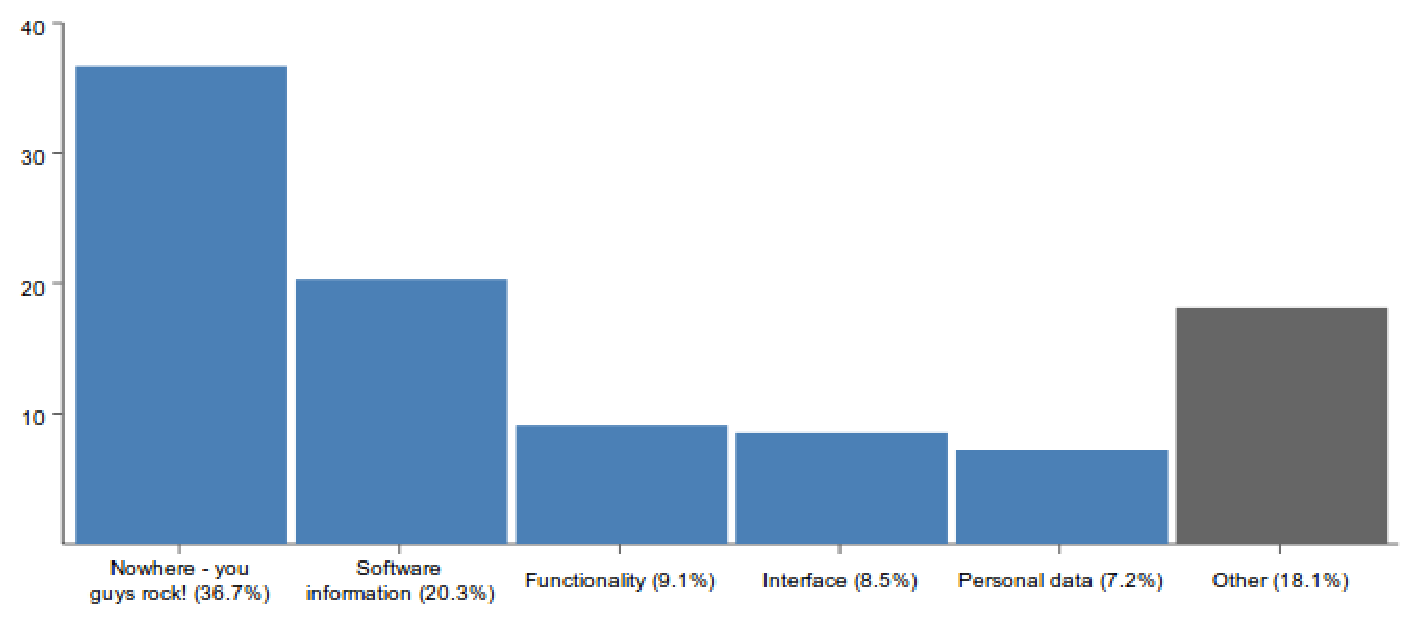
\includegraphics[width=\textwidth]{../images/enquete/improvement}
          \label{fig:improvement}
          \end{center}
        \end{figure}

      Minstens even belangrijk als weten waar mensen enthousiast over zijn is weten waar ze graag verbetering willen zien. Daarom stelde de enqu\^ete de vraag waar de respondenten Wakoopa nog in vonden tekortkomen. De respons hierop is te vinden in figuur \ref{fig:improvement}. Het meest gekozen antwoord was "Nowhere, you guys rock!". 36.7\% van de respondenten had geen grote problemen, of kon er niet direct een noemen. Hoewel dit positief is, zit de waarde van de vraag meer in de andere antwoorden.

      Een groot deel van de respondenten, 20.3\%, vind dat de informatie rondom software te wensen overlaat. Een kijk in het help-forum laat zien dat er inderdaad veel mensen toevoegingen aandragen op dit gebied.\footnote{\url{http://getsatisfaction.com/wakoopa/searches?query=software+information&style=topics}, geraadpleegd op 13 oktober 2009} Wat vaak voorkomt zijn vragen over meer informatie qua versies. Een recente ontwikkeling op dit gebied is dat softwareontwikkelaars nu hun versies en downloads op Wakoopa kunnen beheren, en voor een hogere kwaliteit van informatie kunnen zorgen.

      Een ander veelvoorkomend punt is dat mensen graag specifieke informatie vinden, zoals mogelijke problemen of aandachtspunten. Buiten het reviewsysteem, waar mensen ook opmerkingen of problemen in kunnen vermelden, is hier geen mogelijkheid voor, en er wordt geen interface geboden om deze apart van elkaar, of gesorteerd op versie, te bekijken. Zo'n interface zou een waardevolle toevoeging zijn.


      Hierna vonden de respondenten dat de site te kort kwam op algemene functionaliteit (9\%), de interface (8.5\%) en persoonlijke data (7\%) genoemd. 18.1\% kiest voor other, waarbij om een reden werd gevraagd. Hieronder volgt een greep uit de idee\"en van deze responsen:

      \begin{itemize}
      \item Automatic put a message in twitter
      \item You should translate this webpage into other languages. There is no alternative in, for example, Spanish for software recomendation services. It would be the perfect develope for Wakoopa. Conquer the world!
      \item More intuitive tools to compare and analysis statistics about the software listed. This should include the ability to auto-lookup the names of the apps as the name is being typed.
      \item Social network features: I find the current system pointless and that point system made it even worse, I keep seeing people I don't know add me as a contact.
      \item I think the review system could be updated. It seems that a lot of really low quality reviews get in. Perhaps a rating system that the community could use would fix it.
      \item Software Recommendations. On average I seem accumulate 20 PAGES (far too many) of Software Recommendations. Most of which are awful and irrelevant to my usage. Just because I tried a video editor one time doesn't mean I want recommendations for every lame shareware video editor out there. It would be nice if you guys narrowed it down to 10 recommendations based on the top 10 software I use everyday. Right now it feels like spam.
      \end{itemize}

      Kijkende naar deze replies gaan deze vooral over de \emph{interface}, de presentatie of werking van pagina's. Dit zijn concrete punten, zoals bijvoorbeeld het ratingsysteem. Het ratingsysteem op Wakoopa vraagt gebruikers tussen de nul en vijf sterren te geven. Uit statistieken van Youtube\footnote{\url{http://youtube-global.blogspot.com/2009/09/five-stars-dominate-ratings.html}} blijkt dat voor hun dit model niet werkt. Mensen vinden filmpjes goed en geven dan een vijf, of niet goed en nemen niet de moeite om een review te schrijven. Ook op wakoopa is een soortgelijk patroon te vinden.

      Een usability pattern wat hier rekening mee houd is het `like' pattern, waar mensen enkel aan kunnen geven of ze iets leuk vinden of niet. Op Wakoopa is sinds dit onderzoek een favoriet-functie toegevoegd die dit like-patroon volgt.

      Links met andere sociale netwerken, het uitzenden van software gebruik naar bijvoorbeeld Facebook of Twitter worden ook meerdere malen genoemd. Buiten een Facebook widget en Friendfeed integratie voldoet Wakoopa nog niet aan deze vraag. Het toevoegen van een `share' knop op softwarepagina's heeft tot weinig extra hits geleidt, maar door dit bijvoorbeeld naar `Social' te veranderen, kan door middel van a/b testen worden gegeken of een andere benaming meer effect heeft.

      Een interessant punt is de laatste respons, over het weergeven van minder aanbevelingen. Dit is een paradoxaal punt. Je verwacht dat meer aanbevelingen beter zijn, maar vanuit een gebruikersoogpunt is het wellicht veel interessanter om per categorie een of twee aanbeveling, of een tiental aanbevelingen in totaal te krijgen. Dit creëert het idee dat de aanbevelingen zorgvuldig zijn uitgekozen in plaats van dat er voor alle applicaties wiskundig is gekeken hoeveel het past bij het huidige softwaregebruik van een gebruiker. Omdat de aanbevelingen tweemaal per week veranderen, en er voor wordt gezorgd dat deze niet continue hetzelfde zijn, kan er per week een beperkte set worden weergegeven.

        \begin{figure}
          \begin{center}
          \caption{Wat vinden respondenten van de softwareaanbevelingen?}
            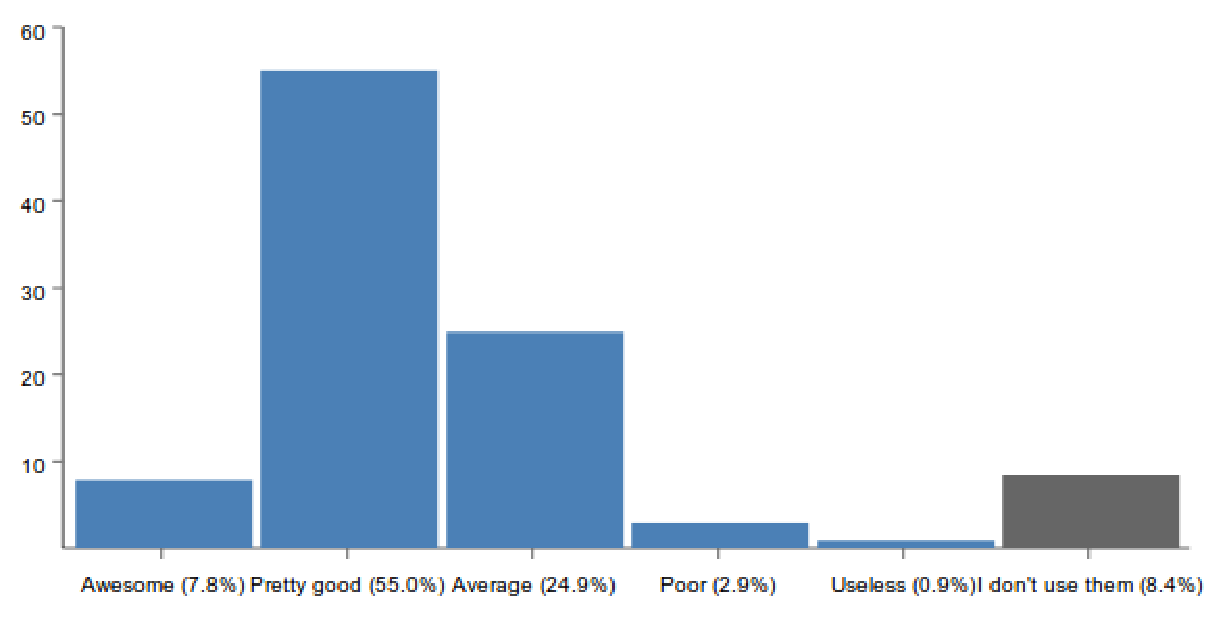
\includegraphics[width=\textwidth]{../images/enquete/think-of-recommendations}
          \label{fig:recommendations}
          \end{center}
        \end{figure}

      \paragraph{}Qua kwaliteit van de aanbevelingen, te zien in figuur \ref{fig:recommendations}, zijn de meeste mensen tevreden. 87.7\% vind de aanbevelingen gemiddeld of bovengemiddeld, en 62.8 vind ze bovengemiddeld goed. een klein percentage van acht-en-een-half procent gebruikt de aanbevelingen in totaal niet. Zoals eerder genoemd zouden we de aanbevelingen exclusiever kunnen laten lijken door er minder tegelijk te laten zien, of per categorie éen aanbeveling te laten zien.

      Uit figuur \ref{fig:advertisements} blijkt dat het overgrote deel van de respondenten de advertenties niet merken of niet als vervelend ervaren. Deze wetenschap kan een rol spelen bij het plaatsen van advertenties op andere pagina's. Wanneer mensen de advertenties op dit moment niet merken, kunnen deze op een zichtbaardere plaats worden neergezet, wat tot een hogere click-through rate zou moeten leiden.

        \begin{figure}
          \begin{center}
          \caption{Wat vinden respondenten van de advertenties}
            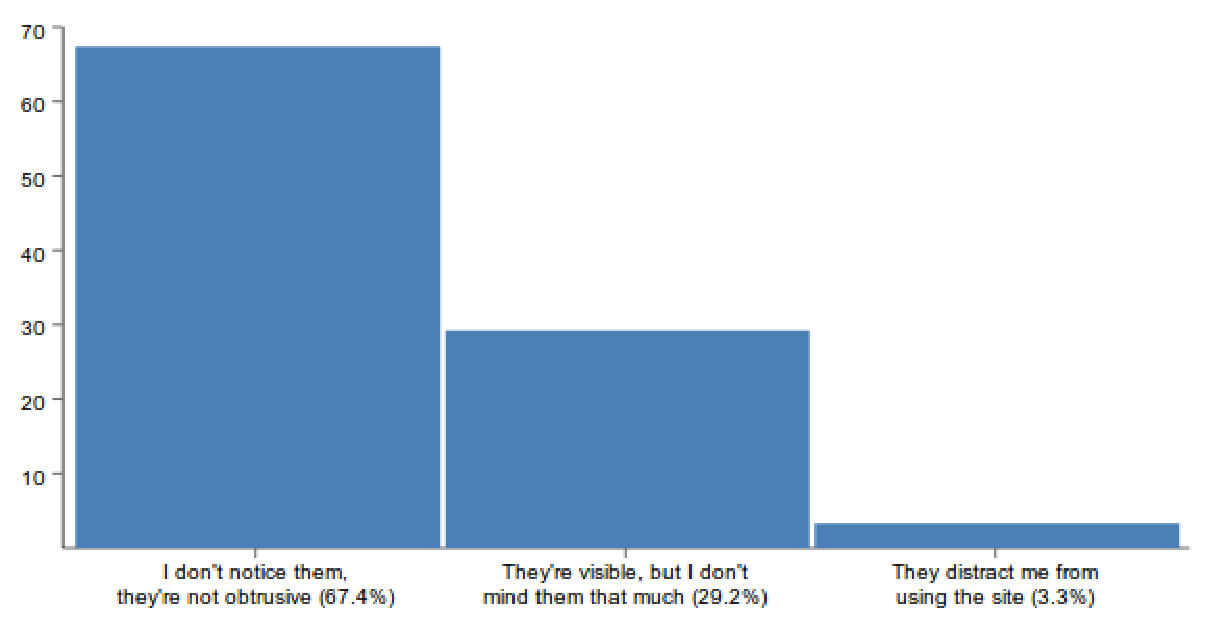
\includegraphics[width=\textwidth]{../images/enquete/advertisements}
          \label{fig:advertisements}
          \end{center}
        \end{figure}


    \label{enqueteappendix}
  \chapter{Persona's}
    \label{personasappendix}
De onderstaande persona's zijn gebaseerd op de interne doelgroepanalyse van Wakoopa en de gegevens uit de uitgevoerde Enqu\^ete.

\section{Tom Daaler}
  \begin{wrapfigure}{l}{40mm}
      
\includegraphics[height=40mm]{../images/personas/tom}
  \end{wrapfigure}
Tom is 17 jaar en zit in zijn laatste jaar havo. Hij werkt als vakkenvuller bij de AH en spendeert de meeste de meeste van zijn vrije tijd achter de pc waar hij games speelt of zijn pc aan het tweaken is. Het geld wat hij bij de AH verdient gaat voornamelijk op aan games en hardware. Hij is nieuwsgierig en probeert daarom vaak nieuwe programma's. Wanneer hij een nieuw programma ontdekt is hij vaak een van de eerste onder zijn vrienden, en is trots als hij zijn bevindingen kan delen en aan anderen uit kan leggen hoe een nieuw programma werkt.

In het MBTI model zoals gebruikt in \cite{Klompsma} is Tom een competetieve bezoeker.

\section{Andreas Nilsson}
  \begin{wrapfigure}{l}{40mm}
      
\includegraphics[height=40mm]{../images/personas/andreas}
  \end{wrapfigure}
Andreas is 28 jaar en heeft een baan bij een IT-bedrijf als programmeur. Buiten zijn werk probeert hij de computer te ontwijken, hoewel hij 's avonds vaak nog even op youtube of hyves zit. Hij wil graag zo efficient mogelijk werken en ergert zich snel aan programma's. Daarintegen wilt hij ook niet teveel tijd besteden aan het vinden en uitzoeken van nieuwe programma's. Het is voor hem belangrijk dat hij zo goed mogelijk zijn werk kan doen en daarbij niet teveel aan andere dingen hoeft te denken. Andreas moet van zijn bedrijf bijhouden waar zijn tijd aan opgaat, iets waar hij eigelijk niet op zit te wachten.

In het MBTI model zoals gebruikt in \cite{Klompsma} is Andreas een competetieve bezoeker.

\section{Johan Broers}
  \begin{wrapfigure}{l}{40mm}
      
\includegraphics[height=40mm]{../images/personas/johan}
  \end{wrapfigure}
Johan is 32 en de maker van TimeSink, een klein programma om je tijd te managen. Hiervan heeft hij een gratis versie en een betaalde versie met meer opties. Naast dit programma werkt hij zelf als freelancer voor verschillende softwarebedrijven, maar het liefst zou hij genoeg verdienen om eigen baas te kunnen worden. hij komt graag in contact met gebruikers van zijn programma en is zeer geinteresseerd in wat ze van zijn programma vinden. Hij kijkt vaak naar zijn downloadstatistieken, maar blijft benieuwd naar hoeveel mensen zijn programma nou echt gebruiken.

In het MBTI model zoals gebruikt in \cite{Klompsma} is Johan een humanistische bezoeker.

\section{Mariette Klompman}
  \begin{wrapfigure}{l}{40mm}
      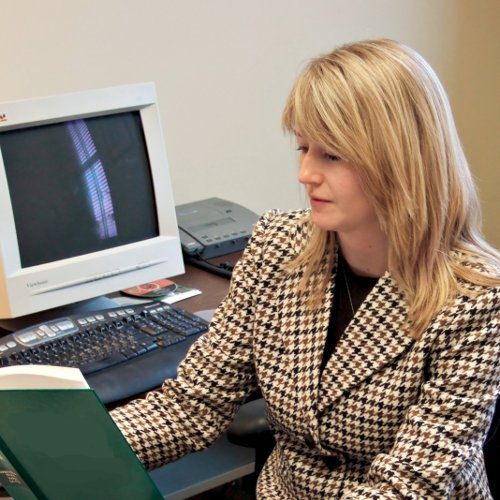
\includegraphics[height=40mm]{../images/personas/mariette}
  \end{wrapfigure}
Mariette is een administratief medewerker voor een scholengemeenschap en moeder van 2 kinderen van 8 en 5. Voor haar werk zit ze veel in microsoft office, maar thuis doet ze eigelijk niks met de computer. In haar vrije tijd loopt ze hard en schildert ze. Ze is niet heel vaardig met computer, ondanks dat ze voor haar werk een cursus office en internet heeft gevolgd. Soms loopt ze vast met word, en vraagt dan haar collega om hulp. Op dagen dat haar collega er niet is, probeerd ze via google toch het antwoord te vinden, maar vaak vind ze niet wat ze zoekt, of ze snapt de gebruikte termen niet helemaal. Als ze het niet snel kan vinden schrijft ze het om op later aan haar collega te vragen en gaat dan ergens anders mee verder.

In het MBTI model zoals gebruikt in \cite{Klompsma} is Mariette een spontane bezoeker.



  \chapter{Lab tests analyses}
    \label{labtestsappendix}

\section{Claudia Engelsman}
\textbf{19 jaar, past bij persona van Mariette.}

\subsection{Opdracht 1}
  Ziet het zoekveld niet en scrollt initieel niet ver genoeg terug naar boven om het te zien. Klikt een aantal keer direct naast het zoekveld op andere opties en komt uiteindelijk op een toplijst, waaruit ze een programma kiest. Eenmaal op de pagina is het schrijven van een review geen probleem

\subsection{Opdracht 2}
  Zoekt naar `websites' in het zoekveld, maar de site reageert erg traag, zo erg dat ze zich afvraagt op het werkt. eenmaal op de zoekpagina klikt ze vrij snel op adobe dreamweaver, totdat ze zich realiseert dat dat geen website is. Ze gaat weg van de zoekpagina en is verward over de verdeling tussen websites en programma's. Via het eigen profiel klikt ze op twitter om dit vervolgens in haar browser toe te voegen als favorite. Hierop heb ik de benaming aangepast

\subsection{Opdracht 3}
  Ze klikt doelgericht naar het eigen profiel en bekijk de pagina. Vervolgens klikt ze bij de grafiek op "today".

\subsection{Opdracht 4}
 Ze klikt direct op people maar kan het daar niet vinden, ze klikt op het dropdown menu van you en op "find en invite people". Ze staat op het punt om het op te geven en klikt door naar het dashboard. Ze zegt dat er wel software recommendations zijn, maar niet gebruikers. Ze scrollt verder naar beneden en meld "oh, ik wist niet dat je ook buren kon hebben", maar ziet dit niet als zijnde `mensen die op je lijken', dit merkt ze ook op. Ze klikt door naar software recommendations, waar "neighbours" wordt uitgelegd. Op het profiel heeft ze geen probleem de persoon als contact toe te voegen.

\subsection{Opdracht 5}
 Ze zoekt teams bij you en bij dashboard, vervolgens bij software en dan naar categorien, die ze als teams ziet. ze klikt door naar een programme en merkt dan op dat het `zeker geen team is'. Ze zoekt in de zoekbalk naar `team', kijkt moeilijk en klikt dan op de teams lijst. Ze zoekt naar twee applicaties, rollercoaster tycoon en spore, waarbij de laatste een team heeft. Eenmaal op de teampagina klikt ze vrij snel op `join this team.'

 \subsection{Algemeen}
  Over het algemeen liggen voor Claudia de meeste problemen in de terminologie en de navigatie. Wanneer ze eenmaal op een pagina zit, vind ze vaak snel waar ze naar zoekt.

\section{Mark van der Ham}
\textbf{20 jaar, past bij persona van Tom.}

\subsection{Opdracht 1}
Klik gelijk door naar Reviews, en zoekt daarna naar Itunes, scrolled vrij lang door de lijst. In de nabespreking gaf hij aan dat het te druk was en dat de verschillende programma's die op itunes leken hem verwarden. Na een aantal keer scrollen klikt hij op de eerste hit. Zodra hij op de itunes pagina zit vind hij het reviewformulier snel

\subsection{Opdracht 2}
Zoek naar een site die niet op wakoopa staat, met de volledige url. Na een opmerking over wat voor sites het moet gaan, zoekt hij op hyves en vind snel de favorite-knop. Vult een erg lange tekst in ondanks het kleine invoerveld.

\subsection{Opdracht 3}
Klik vrij zeker op you, scrollt naar Usage, klikt op Today, maar denkt daarna dat het 'usage in the last hour' het gebruik vandaag is en laat het verder daarbij.

\subsection{Opdracht 4}
Bekijkt vrij lang de persoonlijke profielpagina. Zoekt dan op "developer" en bekijkt het profiel van een van de hits. Gaat dan terug naar het eigen profiel, naar usage and contacts. Zegt dat hij iets van aanbevelingen zoekt maar dat niet kan vinden. Klikt door naar find and invite en ziet dan een link naar recommendations. Leest het tekstje en zegt dat hij het gevonden heeft.

Op het profiel zegt hij dat het al een contact is en wijs op een lege plek naar de block button. Scrollt omlaag en omhoog en ziet dan de "add link".

\subsection{Opdracht 5}
klikt door naar teams, en zoekt naar ultrabeat, waar geen team voor wordt gevonden. Zoekt vervolgens naar 'call of duty' via het zoekveld, die automatisch op software in plaats van developers zoekt. Klikt door naar software, en doet dit een aantal keer. Klik door naar users en merkt op dat het geen team is. Klikt terug naar de teams pagina en klikt op gamers. Op de teampagina klikt hij direct op "join this team".

\subsection{Algemeen}
Mark heeft de dashboard, je eigen startpagina, helemaal niet gezien. Dit had wellicht geholpen bij het vinden van in ieder geval de aanbevelingen. Een grote fout was dat bij het zoeken niet onthouden werd naar wat voor soort dingen gezocht werd, en dat dit er niet duidelijk bovenstond. In opdracht 5 lukte het Mark daarom niet goed een team te vinden.

\section{Mark Dekkers Los}
\textbf{22 jaar, past bij persona van Andreas.}

\subsection{Opdracht 1}
Klik op software en gaat dan naar categories. Vind daar de zoekbalk. Zoekt op quicktime en klikt op het eerste resultaat. Klikt daar gelijk door naar Reviews, en dan in de rechterbovenhoek op "Write one!". Schrijft een review, kijkt even naar de andere reviews en voegt dan ook een rating toe.

\subsection{Opdracht 2}
Klikt op het logo om naar het dashboard, klikt de verschillende menu's aan, en zoekt vervolgens op "website". Zoekt door de resultaten en vindt Facebook. Scrollt over de hele pagina en weer terug, en klikt dan op favorite.

\subsection{Opdracht 3}
Klikt op het profiel en kijkt naar recently used, type of usage and ziet dan "today" bij de grafiek. Klikt op today.

\subsection{Opdracht 4}
Klikt op people, kijkt daar even en wilt gaan zoeken, maar kan niet op een term geven. Vraagt op welke manier ze op elkaar moeten lijken, met het antwoord dat Wakoopa dat aangeeft. Klikt bij people op reviews, en twijfelt vervolgens in het dropdown menu tussen find and invite en recommendations. Klikt op recommendations, vind de neighbours en klikt direct op het toevoegen icoontje.

\subsection{Opdracht 5}
Gaat naar teams, zoekt op "call of duty", merkt op dat het team spaans is en klikt vrij direct op join this team.

\subsection{Algemeen}
Er zijn geen algemeen opvallende dingen aan deze labtest.

\section{Jorn van Schaik}
\textbf{20 jaar, past bij persona van Tom.}

\subsection{Opdracht 1}
Bekijkt het dashboard en klikt op verschillende plekken. Gaat naar het zoekveld en typt dan een zin in, maar zoekt niet. Klikt vervolgens op quicktime player. Geeft later aan dat hij het logischer vondt als je eerst aangaf een review te willen schrijven, en daarna pas waarover in plaats van andersom. Op de softwarepagina vind hij erg snel de review-mogelijkheid.

\subsection{Opdracht 2}
gaat naar het zoekveld en zoekt op een volledige site (url) en vind dan niks. Gaat terug naar de dashboard en klikt dan op "Find and invite". Bekijkt de dropdowns en kijkt verder rond. Vraagt of het op Wakoopa moet. Klikt vervolgens zonder iets te typen op de zoekknop, waardoor er naar "search for..." wordt gezocht. Klikt dan op Google search en vind op de pagina heel snel de favorite knop

\subsection{Opdracht 3}
Klikt direct op de dropdown bij `you' en klikt dan op settings en gaat naar favorites. Bekijkt nogmaals de dropdowns, scrollt naar beneden en klikt op help. Scrollt heen en weer en klikt uiteindelijk op You. Ziet de grafiek, maar selecteert de `top used applications' in plaats van category usage.

\subsection{Opdracht 4}
Klikt direct in de dropdown bij `you' op recommendations, leest het stuk over neighbours, klikt door naar de gebruiker en klikt daar snel op `add as contact'

\subsection{Opdracht 5}
Bekijkt alle dropdowns nogmaals en klikt dan door op `teams'. Bekijkt de pagina maar zoekt niet. Klikt uiteindelijk op een groep en klikt vervolgens direct op `join this team'

\subsection{Algemeen}
Jorn klikte veel en vond daardoor veel functies al voordat hij ze nodig had. Hierdoor kreeg hij snel feeling voor hoe de site in elkaar zat. Opvallend is dat, hoewel hij de zoekfunctie wel heeft gebruikt, en iets in het zoekveld getypt, heeft hij niet bewust naar iets gezocht. Na afloop gaf hij aan dat hij dit gemakkelijker vond.




\end{document}

